% !TeX spellcheck = en_US
% Dieses Dokument muss mit PDFLatex gesetzt werden
% Vorteil: Grafiken koennen als jpg, png, ... verwendet werden
%          und die Links im Dokument sind auch gleich richtig
%
%Ermöglicht \\ bei der Titelseite (z.B. bei supervisor)
%Siehe https://github.com/latextemplates/uni-stuttgart-cs-cover/issues/4
\RequirePackage{kvoptions-patch}

%Englisch:
\let\ifdeutsch\iffalse
\let\ifenglisch\iftrue{}

%Deutsch:
%\let\ifdeutsch\iftrue
%\let\ifenglisch\iffalse

%
\ifdeutsch
	\PassOptionsToClass{numbers=noenddot}{scrbook}
\fi

%Warns about outdated packages and missing caption delcarations
%See https://www.ctan.org/pkg/nag
\RequirePackage[l2tabu, orthodox]{nag}

%Neue deutsche Trennmuster
%Siehe http://www.ctan.org/pkg/dehyph-exptl und http://projekte.dante.de/Trennmuster/WebHome
%Nur für pdflatex, nicht für lualatex
\RequirePackage{ifluatex}
\ifluatex
%do not load anything
\else
	\ifdeutsch
		\RequirePackage[ngerman=ngerman-x-latest]{hyphsubst}
	\fi
\fi

\documentclass[
               fontsize=12pt, %Default: 11pt, bei Linux Libertine zu klein zum Lesen
% BEGINN: Optionen für typearea
               paper=a4,
               twoside, % fuer die Betrachtung am Schirm ungeschickt
               BCOR=3mm, % Hack für BCOR (1.92 o.ä.), da bei BCOR2mm die Fuellpunkte beim Inhaltsverzeichnis falsch sind. Hack aber nicht mehr nötig: microtype für Verzeichnisse ausschalten hilft.
               DIV=13,   % je höher der DIV-Wert, desto mehr geht auf eine Seite. Gute werde sind zwischen DIV=12 und DIV=15
               headinclude=true,
               footinclude=false,
% ENDE: Optionen für typearea
%               titlepage,
               bibliography=totoc,
%               idxtotoc,   %Index ins Inhaltsverzeichnis
%                liststotoc, %List of X ins Inhaltsverzeichnis, mit liststotocnumbered werden die Abbildungsverzeichnisse nummeriert
               headsepline,
               cleardoublepage=empty,
               parskip=half,
%               draft    % um zu sehen, wo noch nachgebessert werden muss - wichtig, da Bindungskorrektur mit drin
               final   % ACHTUNG! - in pagestyle.tex noch Seitenstil anpassen
               ]{scrbook}

%%%
% Beschreibung:
% In dieser Datei werden zuerst die benoetigten Pakete eingebunden und
% danach diverse Optionen gesetzt. Achtung Reihenfolge ist entscheidend!
%
%%%


%%%
% Styleguide:
%
% Ein sehr kleiner Styleguide. Packages werden in Blöcken organisiert.
% Ein Block beginnt mit drei % in einer Zeile, dann % <Blocküberschrift>, dann
% eine Liste der möglichen Optionen und deren Einstellungen, Gründe und Kommentare
% eine % Zeile in der sonst nichts steht und dann wieder %%% in einer Zeile.
%
% Zwischen zwei Blöcken sind 2 Leerzeilen!
% Zu jedem Paket werden soviele Optionen wie möglich/nötig angegeben
%
%%%


%%%
% Codierung
% Wir sind im 21 Jahrhundert, utf-8 löst so viele Probleme.
%
% Mit UTF-8 funktionieren folgende Pakete nicht mehr. Bitte beachten!
%   * fancyvrb mit §
%   * easylist -> http://www.ctan.org/tex-archive/macros/latex/contrib/easylist/
\ifluatex
%no package loading required
\else
\usepackage[utf8]{inputenc}
\fi
%
%%%


%%%
% Deckblattstyle
%
\ifdeutsch
\PassOptionsToPackage{language=german}{uni-stuttgart-cs-cover}
\else
\PassOptionsToPackage{language=english}{uni-stuttgart-cs-cover}
\fi

\newcommand{\docauthor}{Raghuraj Tarikere Phaniraja Setty}
\newcommand{\doctitle}{Space Component Model using DLR Software Technologies}

\usepackage[
title={\doctitle},
author={\docauthor},
type=master,
institute=isterss,
number=12345,
course=se,
examiner={Dr.-Ing.\ Andr\'{e} van Hoorn (Prof.-Vertr.)},
supervisor={Dr.\ Du\v{s}an Okanovi\'{c},\\Teerat Pitakrat,\ M.Sc.},
startdate={October 2, 2017}, % English: July 5, 2013;    ISO: 2013-07-05
enddate={April 2, 2018}, % English: January 5, 2014; ISO: 2014-01-05
crk={I.7.2}
]{uni-stuttgart-cs-cover}
%
%%%


%%%
%Parallelbetrieb tex4ht und pdflatex
\makeatletter
\@ifpackageloaded{tex4ht}{\def\iftex4ht{\iftrue}}
                         {\def\iftex4ht{\iffalse}}
\makeatother
%%%


%%%
%Farbdefinitionen
\usepackage[hyperref,dvipsnames]{xcolor}
%


%%%
% Neue deutsche Rechtschreibung und Literatur statt "Literature", Nachfolger von ngerman.sty
\ifdeutsch
% letzte Sprache ist default, Einbindung von "american" ermöglicht \begin{otherlanguage}{amercian}...\end{otherlanguage} oder \foreignlanguage{american}{Text in American}
% see also http://tex.stackexchange.com/a/50638/9075
\usepackage[american,ngerman]{babel}
% Ein "abstract" ist eine "Kurzfassung", keine "Zusammenfassung"
\addto\captionsngerman{%
	\renewcommand\abstractname{Kurzfassung}%
}
\else
%
%
% if you are writing in english
% last language is the default language
\usepackage[ngerman,american]{babel}
\fi
%
%%%

%%%
% Anführungszeichen
% Zitate in \enquote{...} setzen, dann werden automatisch die richtigen Anführungszeichen verwendet.
\usepackage{csquotes}
%%%


%%%
% erweitertes Enumerate
\usepackage{paralist}
%
%%%


%%%
% fancyheadings (nicht nur) fuer koma
\usepackage[automark]{scrpage2}
%
%%%


%%%
%Mathematik
%
\usepackage[fleqn,leqno]{amsmath} % Viele Mathematik-Sachen: Doku: /usr/share/doc/texmf/latex/amsmath/amsldoc.dvi.gz
%fleqn (=Gleichungen linksbündig platzieren) funktioniert nicht direkt. Es muss noch ein Patch gemacht werden:
\addtolength\mathindent{1em}%work-around ams-math problem with align and 9 -> 10
\usepackage{mathtools} %fixes bugs in AMS math
%
%for theorems, replacement for amsthm
\usepackage[amsmath,hyperref]{ntheorem}
\theorempreskipamount 2ex plus1ex minus0.5ex
\theorempostskipamount 2ex plus1ex minus0.5ex
\theoremstyle{break}
\newtheorem{definition}{Definition}[section]
%
%%%

%%For creating folder structure
\usepackage{dirtree}

\usepackage{forest}
\usetikzlibrary{arrows.meta}
\forestset{
	dir tree/.style={
		for tree={
			parent anchor=south west,
			child anchor=west,
			anchor=mid west,
			inner ysep=1pt,
			grow'=0,
			align=left,
			edge path={
				\noexpand\path [draw, \forestoption{edge}] (!u.parent anchor) ++(1em,0) |- (.child anchor)\forestoption{edge label};
			},
			font=\sffamily,
			if n children=0{}{
				delay={
					prepend={[,phantom, calign with current]}
				}
			},
			fit=band,
			before computing xy={
				l=2em
			}
		},
	}
}

%%%
% Intelligentes Leerzeichen um hinter Abkürzungen die richtigen Abstände zu erhalten, auch leere.
% siehe commands.tex \gq{}
\usepackage{xspace}
%Macht \xspace und \enquote kompatibel
\makeatletter
\xspaceaddexceptions{\grqq \grq \csq@qclose@i \} }
\makeatother
%
%%%


%%%
% Anhang
\usepackage{appendix}
%[toc,page,title,header]
%
%%%


%%%
% Grafikeinbindungen
\usepackage{graphicx}%Parameter "pdftex" unnoetig
\graphicspath{{\getgraphicspath}}
\newcommand{\getgraphicspath}{graphics/}
%
%%%

\usepackage[export]{adjustbox}

%%%
% Enables inclusion of SVG graphics - 1:1 approach
% This is NOT the approach of http://www.ctan.org/tex-archive/info/svg-inkscape,
% which allows text in SVG to be typeset using LaTeX
% We just include the SVG as is
\usepackage{epstopdf}
\epstopdfDeclareGraphicsRule{.svg}{pdf}{.pdf}{%
  inkscape -z -D --file=#1 --export-pdf=\OutputFile
}
%
%%%


%%%
% Enables inclusion of SVG graphics - text-rendered-with-LaTeX-approach
% This is the approach of http://www.ctan.org/tex-archive/info/svg-inkscape,
\newcommand{\executeiffilenewer}[3]{%
\IfFileExists{#2}
{
%\message{file #2 exists}
\ifnum\pdfstrcmp{\pdffilemoddate{#1}}%
{\pdffilemoddate{#2}}>0%
{\immediate\write18{#3}}
\else
{%\message{file up to date #2}
}
\fi%
}{
%\message{file #2 doesn't exist}
%\message{argument: #3}
%\immediate\write18{echo "test" > xoutput.txt}
\immediate\write18{#3}
}
}
\newcommand{\includesvg}[1]{%
\executeiffilenewer{#1.svg}{#1.pdf}%
{
inkscape -z -D --file=\getgraphicspath#1.svg %
--export-pdf=\getgraphicspath#1.pdf --export-latex}%
\input{\getgraphicspath#1.pdf_tex}%
}


%%%
\usepackage{siunitx}
%%%

%%%
\usepackage{acro} %nice Acronyms
%\DeclareAcronym{TCT}{short = TCT , long = task completion time}
%%%


%%%
% Tabellenerweiterungen
\usepackage{array} %increases tex's buffer size and enables ``>'' in tablespecs
\usepackage{longtable}
\usepackage{dcolumn} %Aligning numbers by decimal points in table columns
\ifdeutsch
	\newcolumntype{d}[1]{D{.}{,}{#1}}
\else
	\newcolumntype{d}[1]{D{.}{.}{#1}}
\fi

\usepackage{makecell}

\renewcommand\theadalign{bc}
\renewcommand\theadfont{\bfseries}
\renewcommand\theadgape{\Gape[4pt]}
\renewcommand\cellgape{\Gape[4pt]}

%
%%%

%%%
% Eine Zelle, die sich über mehrere Zeilen erstreckt.
% Siehe Beispieltabelle in Kapitel 2
\usepackage{multirow}
%
%%%

%%%
%Fuer Tabellen mit Variablen Spaltenbreiten
%\usepackage{tabularx}
%\usepackage{tabulary}
%
%%%


%%%
% Links verhalten sich so, wie sie sollen
\usepackage{url}
%
%Use text font as url font, not the monospaced one
%see comments at http://tex.stackexchange.com/q/98463/9075
\urlstyle{same}
%
%Hint by http://tex.stackexchange.com/a/10419/9075
\makeatletter
\g@addto@macro{\UrlBreaks}{\UrlOrds}
\makeatother
%
%%%


%%%
% Index über Begriffe, Abkürzungen
%\usepackage{makeidx} makeidx ist out -> http://xindy.sf.net verwenden
%
%%%

%%%
%lustiger Hack fuer das Abkuerzungsverzeichnis
%nach latex durchlauf folgendes ausfuehren
%makeindex ausarbeitung.nlo -s nomencl.ist -o ausarbeitung.nls
%danach nochmal latex
%\usepackage{nomencl}
%    \let\abk\nomenclature %Deutsche Ueberschrift setzen
%          \renewcommand{\nomname}{List of Abbreviations}
%        %Punkte zw. Abkuerzung und Erklaerung
%          \setlength{\nomlabelwidth}{.2\hsize}
%          \renewcommand{\nomlabel}[1]{#1 \dotfill}
%        %Zeilenabstaende verkleinern
%          \setlength{\nomitemsep}{-\parsep}
%    \makenomenclature
%
%%%

%%%
% Logik für Tex
\usepackage{ifthen} %fuer if-then-else @ commands.tex
%
%%%


%%%
%
\usepackage{listings}
%
%%%


%%%
%Alternative zu Listings ist fancyvrb. Kann auch beides gleichzeitig benutzt werden.
\usepackage{fancyvrb}
%\fvset{fontsize=\small} %Groesse fuer den Fliesstext. Falls deaktiviert: \normalsize
%Funktioniert mit UTF-8 nicht mehr
%\DefineShortVerb{\§} %Somit kann im Text ganz einfach |verbatim| text gesetzt werden.
\RecustomVerbatimEnvironment{Verbatim}{Verbatim}{fontsize=\footnotesize}
\RecustomVerbatimCommand{\VerbatimInput}{VerbatimInput}{fontsize=\footnotesize}
%
%%%


%%%
% Bildunterschriften bei floats genauso formatieren wie bei Listings
% Anpassung wird unten bei den newfloat-Deklarationen vorgenommen
% https://www.ctan.org/pkg/caption2 is superseeded by this package.
\usepackage{caption}
%
%%%


%%%
% Ermoeglicht es, Abbildungen um 90 Grad zu drehen
% Alternatives Paket: rotating Allerdings wird hier nur das Bild gedreht, während bei lscape auch die PDF-Seite gedreht wird.
%Das Paket lscape dreht die Seite auch nicht
\usepackage{pdflscape}
%
%%%


%%%
% Fuer listings
% Wird für fancyvrb und für lstlistings verwendet
\usepackage{float}

%\usepackage{floatrow}
%% zustäzlich für den Paramter [H] = Floats WIRKLICH da wo sie deklariert wurden paltzieren - ganz ohne Kompromisse
% floatrow ist der Nachfolger von float
% Allerdings macht floatrow in manchen Konstellationen Probleme. Deshalb ist das Paket deaktiviert.
%
%%%



%%%
% Fuer Abbildungen innerhalb von Abbildungen
% Ersetzt das Paket subfigure
%
% Due to bug #24 in the caption package we need to update caption3.sty at the moment manualy to use subfig.
% Bug #24: http://sourceforge.net/p/latex-caption/tickets/24/
% corrected caption3.sty: http://sourceforge.net/p/latex-caption/code/HEAD/tree/branches/3.3/tex/caption3.sty
%
\usepackage[caption=false, lofdepth=1, lotdepth]{subfig}
%
%%%




%%%
% Fußnoten
%
%\usepackage{dblfnote}  %Zweispaltige Fußnoten
%
% Keine hochgestellten Ziffern in der Fußnote (KOMA-Script-spezifisch):
%\deffootnote[1.5em]{0pt}{1em}{\makebox[1.5em][l]{\bfseries\thefootnotemark}}
%
% Abstand zwischen Fußnoten vergrößern:
%\setlength{\footnotesep}{.85\baselineskip}
%
%
\renewcommand{\footnoterule}{}             % Keine Trennlinie zur Fußnote
\addtolength{\skip\footins}{\baselineskip} % Abstand Text <-> Fußnote
% Fußnoten immer ganz unten auf einer \raggedbottom-Seite
\usepackage{fnpos}
%
%%%


%%%
%
\raggedbottom     % Variable Seitenhöhen zulassen
%
%%%


%%%
% Falls die Seitenzahl bei einer Referenz auf eine Abbildung nur dann angegeben werden soll,
% falls sich die Abbildung nicht auf der selben Seite befindet...
\iftex4ht
%tex4ht does not work well with vref, therefore we emulate vref behavior
\newcommand{\vref}[1]{\ref{#1}}
\else
\ifdeutsch
\usepackage[ngerman]{varioref}
\else
\usepackage{varioref}
\fi
\fi
%%%

%%%
% Noch schoenere Tabellen als mit booktabs mit http://www.zvisionwelt.de/downloads.html
\usepackage{booktabs}
%
%\usepackage[section]{placeins}
%
%%%


%%%
%Fuer Graphiken. Allerdings funktioniert es nicht zusammen mit pdflatex
%\usepackage{gastex} % \tolarance kann dann nicht mehr umdefiniert werden
%
%%%


%%%
%
%\usepackage{multicol}
%\usepackage{setspace} % kollidiert mit diplomarbeit.sty
%
%http://www.tex.ac.uk/cgi-bin/texfaq2html?label=floats
%\usepackage{flafter} %floats IMMER nach ihrer Deklaration platzieren
%
%%%


%%%
%schoene TODOs
\usepackage{todonotes}
\let\xtodo\todo
\renewcommand{\todo}[1]{\xtodo[inline,color=black!5]{#1}}
\newcommand{\utodo}[1]{\xtodo[inline,color=green!5]{#1}}
\newcommand{\itodo}[1]{\xtodo[inline]{#1}}
%
%%%


%%%
%biblatex statt bibtex
\usepackage[
  backend       = biber, 	%biber dose not work with 64x versions alternative: bibtex8
														%minalphanames only works with biber backend														
  sortcites     = true,
  bibstyle      = alphabetic,
  citestyle     = alphabetic,
  firstinits    = true,
  useprefix     = false, %"von, van, etc." will be printed, too. See below.
  minnames      = 1,
  minalphanames = 3,
  maxalphanames = 4,
  maxbibnames   = 99,
  maxcitenames  = 3,
	natbib        = true,
	eprint        = true,
	url           = true,
  doi           = true,
  isbn          = true,
  backref       = true]{biblatex}
\bibliography{bibliography}
%\addbibresource[datatype=bibtex]{bibliography.bib}

%Do not put "vd" in the label, but put it at "\citeauthor"
%Source: http://tex.stackexchange.com/a/30277/9075
\makeatletter
\AtBeginDocument{\toggletrue{blx@useprefix}}
\AtBeginBibliography{\togglefalse{blx@useprefix}}

%Thin spaces between initials
%http://tex.stackexchange.com/a/11083/9075
\renewrobustcmd*{\bibinitdelim}{\,}

%Keep first and last name together in the bibliography
%http://tex.stackexchange.com/a/196192/9075
\renewcommand*\bibnamedelimc{\addnbspace}
\renewcommand*\bibnamedelimd{\addnbspace}

%Replace last "and" by comma in bibliography
%See http://tex.stackexchange.com/a/41532/9075
\AtBeginBibliography{%
  \renewcommand*{\finalnamedelim}{\addcomma\space}%
}

\DefineBibliographyStrings{ngerman}{
  backrefpage  = {zitiert auf S\adddot},
  backrefpages = {zitiert auf S\adddot},
  andothers    = {et\ \addabbrvspace al\adddot},
  %Tipp von http://www.mrunix.de/forums/showthread.php?64665-biblatex-Kann-%DCberschrift-vom-Inhaltsverzeichnis-nicht-%E4ndern&p=293656&viewfull=1#post293656
  bibliography = {Literaturverzeichnis}
}

%enable hyperlinked author names when using \citeauthor
%source: http://tex.stackexchange.com/a/75916/9075
\DeclareCiteCommand{\citeauthor}
  {\boolfalse{citetracker}%
   \boolfalse{pagetracker}%
   \usebibmacro{prenote}}
  {\ifciteindex
     {\indexnames{labelname}}
     {}%
   \printtext[bibhyperref]{\printnames{labelname}}}
  {\multicitedelim}
  {\usebibmacro{postnote}}

%natbib compatibility
%\newcommand{\citep}[1]{\cite{#1}}
%\newcommand{\citet}[1]{\citeauthor{#1} \cite{#1}}
%Beginning of sentence - analogous to cleveref - important for names such as "zur Muehlen"
%\newcommand{\Citep}[1]{\cite{#1}}
%\newcommand{\Citet}[1]{\Citeauthor{#1} \cite{#1}}
%%%


%%%
% Blindtext. Paket "blindtext" ist fortgeschritterner als "lipsum" und kann auch Mathematik im Text (http://texblog.org/2011/02/26/generating-dummy-textblindtext-with-latex-for-testing/)
% kantlipsum (https://www.ctan.org/tex-archive/macros/latex/contrib/kantlipsum) ist auch ganz nett, aber eben auch keine Mathematik
% Wird verwendet, um etwas Text zu erzeugen, um eine volle Seite wegen Layout zu sehen.
\usepackage[math]{blindtext}
%%%

%%%
% Neue Pakete bitte VOR hyperref einbinden. Insbesondere bei Verwendung des
% Pakets "index" wichtig, da sonst die Referenzierung nicht funktioniert.
% Für die Indizierung selbst ist unter http://xindy.sourceforge.net
% ein gutes Tool zu erhalten
%%%


%%%
%
% hier also neue packages einbinden
%
%%%


%%%
% ggf.in der Endversion komplett rausnehmen. dann auch \href in commands.tex aktivieren
% Alle Optionen nach \hypersetup verschoben, sonst crash
%
\usepackage[]{hyperref}%siehe auch: "Praktisches LaTeX" - www.itp.uni-hannover.de/~kreutzm
%
%% Da es mit KOMA 3 und xcolor zu Problemen mit den global Options kommt MÜSSEN die Optionen so gesetzt werden.
%

% Eigene Farbdefinitionen ohne die Namen des xcolor packages
\definecolor{darkblue}{rgb}{0,0,.5}
\definecolor{black}{rgb}{0,0,0}

\hypersetup{
    breaklinks=true,
    bookmarksnumbered=true,
    bookmarksopen=true,
    bookmarksopenlevel=1,
    breaklinks=true,
    colorlinks=true,
    pdfstartview=Fit,
    pdfpagelayout=SinglePage,
    %
    filecolor=darkblue,
    urlcolor=darkblue,
    linkcolor=black,
    citecolor=black
}
%
%%%


%%%
% cleveref für cref statt autoref, da cleveref auch bei Definitionen funktioniert
\ifdeutsch
\usepackage[ngerman,capitalise,nameinlink,noabbrev]{cleveref}
\else
\usepackage[capitalise,nameinlink,noabbrev]{cleveref}
\fi
%%%


%%%
% Zur Darstellung von Algorithmen
% Algorithm muss nach hyperref geladen werden
\usepackage[chapter]{algorithm}
\usepackage[]{algpseudocode}
%
%%%


%%%
% Schriften
\input{preambel/fonts}
%
%%%


%%%
% Links auf Gleitumgebungen springen nicht zur Beschriftung,
% Doc: http://mirror.ctan.org/tex-archive/macros/latex/contrib/oberdiek/hypcap.pdf
% sondern zum Anfang der Gleitumgebung
\usepackage[all]{hypcap}
%%%


%%%
%Bugfixes packages
%\usepackage{fixltx2e} %Fuer neueste LaTeX-Installationen nicht mehr benoetigt - bereinigte einige Ungereimtheiten, die auf Grund von Rueckwaertskompatibilitaet beibahlten wurden.
%\usepackage{mparhack} %Fixt die Position von marginpars (die in DAs selten bis gar nicht gebraucht werden}
%\usepackage{ellipsis} %Fixt die Abstaende vor \ldots. Wird wohl auch nicht benoetigt.
%
%%%


%%%
% Rand
\input{preambel/margins}
%
%%%


%%%
% Optionen
%
\captionsetup{
  format=hang,
  labelfont=bf,
  justification=justified,
  %single line captions should be centered, multiline captions justified
  singlelinecheck=true
}
%
%neue float Umgebung fuer Listings, die mittels fancyvrb gesetzt werden sollen
\floatstyle{ruled}
\newfloat{Listing}{tbp}{code}[chapter]
\crefname{Listing}{Listing}{Listings}
\newfloat{Algorithmus}{tbp}{alg}[chapter]
\ifdeutsch
\crefname{Algorithmus}{Algorithmus}{Algorithmus}
\else
\crefname{Algorithmus}{Algorithm}{Algorithms}
\fi
%
%amsmath
%\numberwithin{equation}{section}
%\renewcommand{\theequation}{\thesection.\Roman{equation}}
%
%pdftex
\pdfcompresslevel=9
%
%Tabellen (array.sty)
\setlength{\extrarowheight}{1pt}
%
%
%%%

%%%
% unterschiedliche Chapter-Styles
% u.a. Paket fncychap
\input{preambel/chapterheads}
%%%

%%%
%Minitoc-Einstellungen
%\dominitoc
%\renewcommand{\mtctitle}{Inhaltsverzeichnis dieses Kapitels}
%
% Disable single lines at the start of a paragraph (Schusterjungen)
\clubpenalty = 10000
%
% Disable single lines at the end of a paragraph (Hurenkinder)
\widowpenalty = 10000 \displaywidowpenalty = 10000
%
%http://groups.google.de/group/de.comp.text.tex/browse_thread/thread/f97da71d90442816/f5da290593fd647e?lnk=st&q=tolerance+emergencystretch&rnum=5&hl=de#f5da290593fd647e
%Mehr Infos unter http://www.tex.ac.uk/cgi-bin/texfaq2html?label=overfull
\tolerance=2000
\setlength{\emergencystretch}{3pt}   % kann man evtl. auf 20 erhoehen
\setlength{\hfuzz}{1pt}
%
%%%


%%Tightly pack diagrams
\usepackage[caption=false]{subfig}

%%%
% Fuer listings.sty
\lstset{language=XML,
        showstringspaces=false,
        extendedchars=true,
        basicstyle=\footnotesize\ttfamily,
        commentstyle=\slshape,
        stringstyle=\ttfamily, %Original: \rmfamily, damit werden die Strings im Quellcode hervorgehoben. Zusaetzlich evtl.: \scshape oder \rmfamily durch \ttfamily ersetzen. Dann sieht's aus, wie bei fancyvrb
        breaklines=true,
        breakatwhitespace=true,
        columns=flexible,
        aboveskip=0mm, %deaktivieren, falls man lstlistings direkt als floating object benutzt (\begin{lstlisting}[float,...])
        belowskip=0mm, %deaktivieren, falls man lstlistings direkt als floating object benutzt (\begin{lstlisting}[float,...])
        captionpos=b
}
\ifdeutsch
\renewcommand{\lstlistlistingname}{Verzeichnis der Listings}
\fi
%
%%%


%%%
%fuer algorithm.sty: - falls Deutsch und nicht Englisch. Falls Englisch als Sprache gewählt wurde, bitte die folgenden beiden Zeilen auskommentieren.
\floatname{algorithm}{Algorithmus}
\ifdeutsch
\renewcommand{\listalgorithmname}{Verzeichnis der Algorithmen}
\fi
%
%%%


%%%
% Das Euro Zeichen
% Fuer Palatino (mathpazo.sty): richtiges Euro-Zeichen
% Alternative: \usepackage{eurosym}
\newcommand{\EUR}{\ppleuro}
%
%%%


%%%
%
% Float-placements - http://dcwww.camd.dtu.dk/~schiotz/comp/LatexTips/LatexTips.html#figplacement
% and http://people.cs.uu.nl/piet/floats/node1.html
\renewcommand{\topfraction}{0.85}
\renewcommand{\bottomfraction}{0.95}
\renewcommand{\textfraction}{0.1}
\renewcommand{\floatpagefraction}{0.75}
\setcounter{secnumdepth}{3}
\setcounter{tocdepth}{3}
%
%%%

%%%
%
% Bei Gleichungen nur dann die Nummer zeigen, wenn die Gleichung auch referenziert wird
%
% Funktioniert mit MiKTeX Stand 2012-01-13 nicht. Deshalb ist dieser Schalter deaktiviert.
%
%\mathtoolsset{showonlyrefs}
%
%%%


%%%
%ensure that floats covering a whole page are placed at the top of the page
%see http://tex.stackexchange.com/a/28565/9075
\makeatletter
\setlength{\@fptop}{0pt}
\setlength{\@fpbot}{0pt plus 1fil}
\makeatother
%%%


%%%
%Optischer Randausgleich
\usepackage{microtype}
%%%

%%%
%Package geometry to enlarge on page
%
%Source: http://www.howtotex.com/tips-tricks/change-margins-of-a-single-page/
%
%Normally, this should not be used as the typearea package calculates the margins perfectly
\usepackage[
  pass %just load the package and do not destory the work of typearea
]{geometry}
%%%


%Der untere Rand darf "flattern"
\raggedbottom

%%%
% Wie tief wird das Inhaltsverzeichnis aufgeschlüsselt
% 0 --\chapter
% 1 --\section % fuer kuerzeres Inhaltsverzeichnis verwenden - oder minitoc benutzen
% 2 --\subsection
% 3 --\subsubsection
% 4 --\paragraph
\setcounter{tocdepth}{1}
%
%%%

\makeindex

%Angaben in die PDF-Infos uebernehmen
\makeatletter
\hypersetup{
            pdftitle={\doctitle}, %Titel der Arbeit
            pdfauthor={\docauthor}, %Author
            pdfkeywords={}, % CR-Klassifikation und ggf. weitere Stichworte
            pdfsubject={}
}
\makeatother


%%% acro
% alle Acronyme die verwendet werden kommen hier her.

\DeclareAcronym{ER}{short = ER , long = error rate}
\DeclareAcronym{FR}{short = FR , long = Fehlerrate}

%%%


\begin{document}

%tex4ht-Konvertierung verschönern
\iftex4ht
% tell tex4ht to create picures also for formulas starting with '$'
% WARNING: a tex4ht run now takes forever!
\Configure{$}{\PicMath}{\EndPicMath}{} 
%$ % <- syntax highlighting fix for emacs
\Css{body {text-align:justify;}}

%conversion of .pdf to .png
\Configure{graphics*}  
         {pdf}  
         {\Needs{"convert \csname Gin@base\endcsname.pdf  
                               \csname Gin@base\endcsname.png"}%  
          \Picture[pict]{\csname Gin@base\endcsname.png}%  
         }  
\fi

%Tipp von http://goemonx.blogspot.de/2012/01/pdflatex-ligaturen-und-copynpaste.html
%siehe auch http://tex.stackexchange.com/questions/4397/make-ligatures-in-linux-libertine-copyable-and-searchable
%
%ONLY WORKS ON MiKTeX
%On other systems, download glyphtounicode.tex from http://pdftex.sarovar.org/misc/
%
%input glyphtounicode.tex
\pdfgentounicode=1

\VerbatimFootnotes %verbatim text in Fußnoten erlauben. Geht normalerweise nicht.

%wird fuer Tabellen benötigt (z.B. >{centering\RBS}p{2.5cm} erzeugt einen zentrierten 2,5cm breiten Absatz in einer Tabelle
\newcommand{\RBS}{\let\\=\tabularnewline}

\newcommand{\source}[1]{\caption*{Source: {#1}} }

%% typoraphisch richtige Abkürzungen
\newcommand{\zB}[0]{z.\,B.\xspace}
\newcommand{\bzw}[0]{bzw.\xspace}
\newcommand{\usw}[0]{usw.\xspace}
\renewcommand{\dh}[0]{d.\,h.\xspace}

%from hmks makros.tex - \indexify
\newcommand{\toindex}[1]{\index{#1}#1}
%
\newcommand{\dotcup}{\ensuremath{\,\mathaccent\cdot\cup\,}} %Tipp aus The Comprehensive LaTeX Symbol List
%
%Anstatt $|x|$ $\abs{x}$ verwenden. Die Betragsstriche skalieren automatisch, falls "x" etwas größer sein sollte...
\newcommand{\abs}[1]{\left\lvert#1\right\rvert}
%
%für Zitate
\newcommand{\citeS}[2]{\cite[S.~#1]{#2}}
\newcommand{\citeSf}[2]{\cite[S.~#1\,f.]{#2}}
\newcommand{\citeSff}[2]{\cite[S.~#1\,ff.]{#2}}
\newcommand{\vgl}{vgl.\ }
\newcommand{\Vgl}{Vgl.\ }
%
\newcommand{\commentchar}{\ensuremath{/\mkern-4mu/}}
\algrenewcommand{\algorithmiccomment}[1]{\hfill $\commentchar$ #1}

% Seitengrößen - Gegen Schusterjungen und Hurenkinder...
\newcommand{\largepage}{\enlargethispage{\baselineskip}}
\newcommand{\shortpage}{\enlargethispage{-\baselineskip}}

\pagenumbering{roman}
\Titelblatt

%Eigener Seitenstil fuer die Kurzfassung und das Inhaltsverzeichnis
\deftripstyle{preamble}{}{}{}{}{}{\pagemark}
%Doku zu deftripstyle: scrguide.pdf
\pagestyle{preamble}
\renewcommand*{\chapterpagestyle}{preamble}

\section*{Abstract}
... Short summary of the thesis in English ...
\cleardoublepage

\section*{Kurzfassung}
... Short summary of the thesis in German ...
\cleardoublepage

% BEGIN: Verzeichnisse

\iftex4ht
\else
\microtypesetup{protrusion=false}
\fi

%%%
% Literaturverzeichnis ins TOC mit aufnehmen, aber nur wenn nichts anderes mehr hilft!
% \addcontentsline{toc}{chapter}{Literaturverzeichnis}
%
% oder zB
%\addcontentsline{toc}{section}{Abkürzungsverzeichnis}
%
%%%

%Produce table of contents
%
%In case you have trouble with headings reaching into the page numbers, enable the following three lines.
%Hint by http://golatex.de/inhaltsverzeichnis-schreibt-ueber-rand-t3106.html
%
%\makeatletter
%\renewcommand{\@pnumwidth}{2em}
%\makeatother
%
\tableofcontents

% Bei einem ungünstigen Seitenumbruch im Inhaltsverzeichnis, kann dieser mit
% \addtocontents{toc}{\protect\newpage}
% an der passenden Stelle im Fließtext erzwungen werden.

\listoffigures
\listoftables

\ifdeutsch
\printacronyms[name=Abkürzungsverzeichnis, heading=chapter*]
\else
\printacronyms[name=List of Acronyms, heading=chapter*]
\fi

%Wird nur bei Verwendung von der lstlisting-Umgebung mit dem "caption"-Parameter benoetigt
%\lstlistoflistings 
%ansonsten:
\ifdeutsch
\listof{Listing}{Verzeichnis der Listings}
\else
\listof{Listing}{List of Listings}
\fi

%mittels \newfloat wurde die Algorithmus-Gleitumgebung definiert.
%Mit folgendem Befehl werden alle floats dieses Typs ausgegeben
\ifdeutsch
\listof{Algorithmus}{Verzeichnis der Algorithmen}
\else
\listof{Algorithmus}{List of Algorithms}
\fi
%\listofalgorithms %Ist nur für Algorithmen, die mittels \begin{algorithm} umschlossen werden, nötig

\iftex4ht
\else
%Optischen Randausgleich und Grauwertkorrektur wieder aktivieren
\microtypesetup{protrusion=true}
\fi

% END: Verzeichnisse

\mainmatter
\pagenumbering{arabic}

\renewcommand*{\chapterpagestyle}{scrplain}
\pagestyle{scrheadings}
\input{preambel/pagestyle}
%
%
% ** Hier wird der Text eingebunden **
%
% !TeX spellcheck = en_US

\chapter{Introduction}
\label{chap: Introduction}
\section{Motivation}
European space industry has entered an economic era in which the funding availed to future space missions are not expected to grow significantly. At the same time, future missions are expected to achieve more and more challenging scientific goals with upcoming seasons of capped budgets for earth observation, scientific studies and space exploration \cite{PhdThesis}. This leads to a situation where the activities like mission analysis and system engineering will play a bigger role in the overall economy of the project, with a proportional increase of the time and cost invested in them \cite{PhdThesis}. The implication of this is that the realization activities, and software development among them are pushed forward in the project schedule and compressed \cite{SAVOIR}. Also, the complexity of the software product is foreseen to increase significantly to keep pace with rising mission needs, while the cost of the software development is expected to fit in the same or perhaps even decreased budget envelope. This situation is therefore calling for a rise in the cost effectiveness of the software development, thus ultimately increasing the "value" of the software product delivered with a given budget.

On-board software for satellites can be classified as high-integrity real-time software and the realization of the functional contents which add "value" to the product, is subject to stringent requirements at both process and product level in dimensions such as: time and space predictability, safety, dependability, security \cite{PhdThesis}. Also the software product is subject to extensive verification and validation steps to ascertain its quality \cite{SAVOIR}. In order to achieve all of this at reduced effort and a constant overall budget and at an acceptable level of quality, the concept of reusable software architecture plays a crucial role. In this context, a software architecture expresses an architectural framework that hosts the functional contents, architectural assumptions and methodological principles that majorly contribute to the attainment of the desired quality of the software product \cite{PhdThesis}.

Parallely in the automotive domain, innovative vehicle functions are leading to a continual increase in the complexity of the vehicle architecture. At the same time, requirements are also sometimes contradictory, for example, supporting driver assistance systems in critical driving manoeuvers while also improving fuel economy and also conforming to the environmental standards \cite{AUTOSARurl}. Additional challenges include deeper integration of the infotainment and communication with the immediate vehicle environment and with online services. In order to continue to meet these requirements in the future, a new technological approach is required for the ECU software architecture \cite{AUTOSARurl}.  

More insights into the concepts of software architecture and a software reference architecture are given in the subsequent chapters.     

The initiatives in coming up with a software architecture in both space and automotive industries adopt the approaches based on the \ac{cbse} and \ac{mde}, which are in recent times gaining huge industrial acceptance in the domain of embedded real-time systems. This is not surprise at all since these two development paradigms promise important advantages such as better and more disciplined software design and increased reuse potential for the former; greater abstraction level and powerful automation capabilities for the latter \cite{CBSE}\cite{PhdThesis}. Many domain specific initiatives have shown that the the higher level of abstraction in the design process facilitated by the MDE allows addressing the non-functional concerns earlier in the development, thereby enabling proactive analysis, maturation and consolidation of the software design \cite{CompBasedDev}. Moreover, the automation capabilities of the MDE infrastructure may ease the generation of lower-level design artifacts and ease the generation of source code products.
Taking first steps towards such an automation is the main motivation for this Master thesis.

\section{Thesis Structure}
This Master thesis is organized into following chapters:
\begin{description}
\item[Chapter~\ref{chap:OSRA} -- \nameref{chap:OSRA}:] This chapter gives an overall idea of a software architecture and a software reference architecture. It also explains the need for \ac{osra}, user needs and high level requirements which led to the development of OSRA and the overall software architectural concept defined in the development of OSRA.  
\item[Chapter~\ref{chap: Software development process} -- \nameref{chap: Software development process}:] This chapter explains in detail; the design and implementation steps for the \ac{cbse} approach which are enforced as a result of adoption of OSRA and its principles.
\item[Chapter~\ref{chap: Tasking framework} -- \nameref{chap: Tasking framework}:] This chapter explains the Tasking framework which is a portable framework for data flow and event driven cooperative multitasking.    
\item[Chapter~\ref{chap: Progamming model} -- \nameref{chap: Progamming model}:] This chapter aims at developing a programming model for this Master thesis. 
\item[Chapter~\ref{chap: Code generation} -- \nameref{chap: Code generation}:] This chapter deals with the mapping of \ac{obsw} model entities to the infrastructural code entities which are generated by a prototypical code generator, which is developed as a part of this Master thesis.
\item[Chapter~\ref{chap: code generator evaluation} -- \nameref{chap: code generator evaluation}:] This chapter subjects the prototypical code generator developed in this Master thesis to a tool acquisition evaluation using certain well defined evaluation methods. 
\item[Chapter~\ref{chap:conclusion} -- \nameref{chap:conclusion}:] This chapter contains discussions about the conclusions derived from the Master thesis and charts the future work plan and enhancements to this Master thesis.
\item[Appendix~\ref{chap: File structure} -- \nameref{chap: File structure}:] This section gives an idea of how the generated code for OBSW models can be organized into different files and folders.
\item[Appendix~\ref{chap: Extra examples} -- \nameref{chap: Extra examples}:] This section lists all the additional example \ac{obsw} models for which the code generator developed as a part of this Master thesis is tested.
\end{description}

%\input{...further chapters...}
% !TeX spellcheck = en_US

\chapter{The On-board Software Reference Architecture (OSRA)}
\label{chap:OSRA}
\section{Introduction}
\subsection{Background}
Space industry has recognized for the past decade the need to raise the level of standardization in the avionics system in order to increase the efficiency and reduce cost and schedule in the development \cite{SAVOIR}.
The implementation of such a vision is expected to provide benefits for all the stake-holders in the space community \cite{SAVOIR}.

\begin{description}
\item  [Customer Agencies] Significant reduction in the project development cost and schedule and the risk involved in the software development
\item [System Integrators] Increased competition among stake-holders to deliver at lower price and maintain shorter time-to-market as a result of multi-supplier option
\item [Supplier Industry] Benefits from diversified customer bases and the supplied building blocks would be compatible with software architectures from the software primes such as Thales Alenia Space and astrium Satellites (EADS Astrium)
\end{description}

Similar initiatives have already been taken across various industries and eg. \ac{autosar} for the automotive industry is worthy mentioning \cite{BasConAUTOSAR}. Space can benefit from these examples by studies related to how these or similar initiatives were successfully conducted and how they faired. Although the business model is different in the automotive and the space sectors, AUTOSAR demonstrates that the need for standardization is the key irrespective of the sector and is driven by the need of the industry to become more competitive \cite{EfAnAUTOSAR}

Space primes and on-board software companies have made significant progress and have implemented and/or are implementing reuse on the basis of their internal software reference architectures and building blocks. However, for this standardization to provide maximum benefits, it has to be tackled at the European level rather than at company level \cite{SAVOIR}

\ac{esa} through its two parallel activities, namely \ac{cordet} and \ac{domeng} \cite{CORDET} aimed at increasing the software reuse in on-board software have confirmed that interface standardization allows to efficiently compose the software on the basis of existing and mature building blocks.

To refer to all ongoing initiatives and to provide a platform for technical discussions, related to the vision of avionics development through maximizing reuse and standardization, a \ac{savoir} Advisory Group (SAVOIR Advisory Group) was created. SAVOIR Advisory Group decided to spawn a specific subgroup for on-board software reference architectures called "SAVOIR Fair Architecture and Interface Reference Elaboration"(SAVOIR FAIRE) working group. \ac{osra} is the result of the R\&D activities of this group \cite{SAVOIR}.   

The OSRA is designed to be a single, common and agreed framework for the definition of the \ac{obsw} of the future European Space Agency (ESA) missions \cite{SAVOIR}. It is based on solid scientific foundations and accompanied by development methodology and architectural practices that fit the domain. A single software system would thus be an "instantiation" of the reference architecture to specific mission needs.

\section{Need for software reference architecture}
\subsection{Motivation}
According to the ISO/IEC standard ISO 42010 \cite{ISO42010}, the software architecture is defined as: 

\textit{"The fundamental organization of a system embodied in its components, their relationships
to each other, and to the environment, and the principles guiding its design and evolution"}
 
A software architecture is the key to create "good quality" software because it promotes architectural best practices and contributes to the quality of the software. A bad architecture hinders the fulfillment of functional, behavioral, non-functional and life-cycle requirements.

According to the "\ac{rup}" \cite{RUP}, the software reference architecture can be defined as:

\textit{"a predefined architectural pattern, or set of patterns, possibly partially or
completely instantiated, designed, and proven for use in particular business and technical contexts, together with supporting artifacts to enable their use. Often, these artifacts are harvested
from previous projects"} 

A software reference architecture prescribes the form of concrete software architectures for a set of systems for which it was developed. So, a reference architecture is a form of "generic" software architecture which prescribes the founding principles, the underlying methodology and the architectural practices that were recognized by the domain stakeholders as the best solution to the construction of a certain class of software systems  \cite{PhdThesis}\cite{SoftRefArch}.

Elevating a software architecture to a software reference architecture permits to gather and re-use lessons learned and architectural best practices, give new projects a consolidated running start and promote a product line approach \cite{SAVOIR}.

A generic software reference architecture is made up of two main parts: \cite{SAVOIR}

\begin{itemize}
\item A software architectural concept addressing the pure software architectural related issues
\item Architectural building blocks related to functional aspects and the corresponding interface definitions which express functions derived from the analysis of the functional chains of the core on-board software domain 
\end{itemize}

\begin{figure}[h]
	\centering
	
\includegraphics[width=0.8\textwidth]{SoftwareReferenceArchitecture.pdf}
	\caption{Parts of a software reference architecture}
	\source{\cite{SAVOIR}}
	\label{}
\end{figure} 

As mentioned in the previous section, in order to increase the efficiency and cost-effectiveness in the development process of on-board avionics and to incorporate more number of functionality in the on-board software, the overall objective of space industry would be to standardize the avionics systems and therefore the on-board software.

A building block approach is one of the ways to tackle this problem. In this approach, the on-board software is implemented from a set of pre-developed and compatible building blocks, plus specific adaptations and "missionisation" according to specific mission requirements \cite{SAVOIR}. The target missions are the core ESA missions, i.e. high reliability and availability spacecraft driven systems (eg. operational missions, science missions).

The "right" building blocks need to be produced and supplied by the suppliers to any system integrator and to achieve this, reference architectures need to be defined.

A software building block, generally:
\begin{itemize}
\item Has a clear, well defined, specified, documented function and open external interfaces for the purpose of interaction
\item Meets defined performance, operation and other requirements
\item Is self-contained so that they can be used at higher-integration levels eg. board, equipment, subsystem 
\item Has a quality level that can be assessed
\item Is applicable in well defined physical and hardware environment
\item Is worth developing as they are going to be used in bulk of ESA missions
\item Is designed for reuse in different projects, by different users under different environments
\item Can be made available off-the-shelf, read for deployment under different conditions.  
\end{itemize}

Separation of the application aspects from the general-purpose data processing aspects is the key to generic/reusable software architectures \cite{PhdThesis}. The lower layers of the architectures usually handle the implementation of communication, real time capabilities etc. and the higher level layers usually deal with the application aspects. However there have to be ways to annotate the application building blocks (ABB) with sufficient information regarding requirements related to communication, real-time, dependability etc., so that the platform building blocks (PBB) can provide the suitable complete implementation. Development of interface specifications with reference architectures as the basis allows the implementation of the famous AUTOSAR concept: \textit{"Cooperate on standards, compete on implementation"}\cite{AUTOSARurl}

The OBSW life-cycle needs to be consistent with the system life-cycle, which features the definition of functional increments in system development \cite{SAVOIR}. Hence, OBSW must in particular:

\begin{itemize}
\item Allow for faster software development
\item Be compatible to a late definition or changes of some of its requirements
\item Cope with various system integration strategies
\end{itemize}

\subsection{User needs}

The COrDeT study, with the slogan "Faster, Later, Software", represented a summary of the above programmatic stakes for the on-board-software life-cycle \cite{CORDET}\cite{SAVOIR}. These stakes are included and defined as the user needs \cite{SAVOIR}\cite{PhdThesis} for the development of OSRA:

\begin{description}
\item [Shorter software development time] Need for faster software development in the context of a shorter schedule. The \cref{fig:RedSWSched} depicts the reduction in the schedule for software development in the future projects. 

\begin{figure}[h]
	\centering
	\includegraphics[width=0.8\textwidth]{ReductionSWSchedule.pdf}
	\caption{Reduction in the schedule for software development}
	\source{\cite{SAVOIR}}
	\label{fig:RedSWSched}
\end{figure}

\item [Reduce recurring costs] Identification and reduction of recurring costs by providing the same set of functions eg. device drivers, real-time operating systems, communication services etc.   

\item [Quality of the product] Need for high quality software (timing predictability, dependability, etc.) and the quality must be at least the same as one of OBSW developed with current approaches.

\item [Increase cost-efficiency] Increase in the "value" of the software product that is developed for a given amount of budget.

\item [Reduce Verification and Validation effort] The new development approaches shall foster the reduction of effort for \ac{vandv} efforts, which is one of the main contributor to the cost of software development.

\item [Mitigate the impact of late requirement definition or change] 

\item [Support for various system integration strategies] It should be possible to do preliminary software releases which allow early system integration efforts.

\item [Simplification and harmonization of FDIR] A simplification and hopefully, harmonization of the \ac{fdir} approach is advocated.

\item [Optimize flight maintenance] There should be provision for changing the OBSW during flight maintenance and coordination of strategies to perform it. 

\item [Industrial policy support] Enable multi-team software development, so that sub-contracting to the non-primes is possible, while still being in-charge of the integration.

\item [Role of software suppliers] Increase competence of supplier and foster competition among them. 

\item [Dissemination activities] System engineers should be exposed to the core principles of the process.

\item [Future needs] Future needs such as integration of functions of different criticality and security levels, use of Time and Space Partitioning (TSP), support to multi-core processors, need to subjected to evaluation and their impact on software reference architecture need to be monitored.
\end{description} 

\subsection{High level requirements}
\label{subsection: High level requirements}
The user needs are translated into a set of high-level requirements for OSRA \cite{SAVOIR}\cite{PhdThesis}.

\begin{description}
\item [Software reuse] The architecture shall be designed in such a way that the reuse of the functional aspects should be independent of the reuse of the non-functional aspects, reuse of the unit, integration and validation tests are made possible.
 
\item [Separation of concerns] Separation of concerns is one of the cornerstone principles of OSRA and it deals with separating different aspects of the software design, in particular the functional and non-functional concerns. Separation of concerns helps to reuse functional concerns independently from non-functional concerns, which increases the software reuse.
 
\item [Reuse of V\&V tests] The chosen architectural approach should also promote the reuse of Verification and Validation tests that were performed on the software and not just the software itself. The aim is to maximize the reuse of the tests written for the functional part of the component software.

\item [HW/SW Independence] Software should be developed independent from the hardware features. It is necessary to separate parts of the software that interact directly with the hardware, into separate modules and make them accessible through defined interfaces. In this way, as long as the interface does not change, the software is isolated from the changes in the hardware-dependent layers.
	  	
\item [Component based approach] The whole software should be designed as a composition of components that are reusable in nature. The architecture shall respect preservation of properties of individual building blocks, once they are integrated into the architecture and it should be possible to calculate the system's property as a function of components' individual properties. The former is called composability and the latter is called compositionality \cite{CompBasedDev}. Chapter \cref{chap: Software development process} explains this approach in more detail.
  
\item [Software observability] The software architecture should provide means to observe the software specific parts and extract current and past status of the software using the services specified by its operational scenarios.

\item [Software analysability] The design process and methodology used for the reference architecture shall support the verification of functional and non-functional properties at design time.

\item [Property preservation] The non-functional properties should be considered as constraints on the system as they specify the "frame" in which the system is expected to behave. 
These properties have to be preserved or enforced so that these properties are not only used for the analysis of the software model, but also find their way through to the final system at run-time. Adequate mechanisms should be provided to handle the enforcement of the properties and also mechanisms to handle reactions to violation of these properties. 

\item [Integration of software building blocks] The architecture should allow the combination of coherent building blocks.

\item [Support for variability factors] The architecture shall include design features allowing isolating the variability foreseen in the domain of reuse.

\item [Late incorporation of modification in the software] The architecture should be immune to late modification of the software in the software life-cycle. System integration almost always finds some system problems and it is the responsibility of the software to contain these problems and implement new requirements. The architecture to which the software is conformal to, should be able to handle these late modifications in the software.

\item [Provision of mechanisms for FDIR] The requirements for FDIR, are consolidated often late in the life cycle and the software architecture must accommodate for it.

\item [Software update at run-time] The reference architecture should allow update to single software components as well as their bindings without having to reboot the entire on-board computer as it is a risk for the system and reduces the mission availability/up-time.
\end{description}  

\section{The Software Architectural Concept}
\subsection{Fitting Model-Driven Engineering}
\ac{mde} is a novel trend for software development in the space domain, but has been successfully applied to enterprise computing \cite{CompBasedDev}. The validation-intensive real-time high-integrity systems such as on-board software systems make the adoption of the MDE considerable more arduous. Positive experiences on the application of MDE to the design of these kind of systems do exist and it can be found in the '\ac{chess}: space case study' \cite{CompBasedProcess} and the 'ESA: reference Earth Observation case study' \cite{CompBasedProcess}.

In MDE, the principal design artifact is a model, which is an abstract representation of the system under development which encompasses systems and software architecture. Each model conforms with a metamodel, which describes the syntax of entities that populate the models, as well as their relationships and the constraints in place between them. The metamodel constrains the design space of the MDE infrastructure \cite{Metamodelling}.  

COrDeT (Component Oriented Development Techniques) aimed at investigating various techniques in fields such as software product line engineering, model driven engineering and component orientation \cite{CORDET}. Based on this study, the concept of overall software reference architecture, in the development of OSRA, is considered to be made up of \cite{SoftRefArch}\cite{SAVOIR}:

\begin{description}
\item [Component Model] A component model is the basis for designing the software as a composition of individually verifiable and reusable software units \cite{ComponentModel}.

\item [Computational Model] A computational model is used to relate to the design entities of the component model, their non-functional needs for concurrency, time and space, to a framework consisting of analysis techniques, in general, to a set of schedulability analysis equations, which help to judge formally, whether the description of the architecture is statically analyzable \cite{ScheduAnaly}

\item [A Programming Model] A programming model is used to ensure that the implementation of the design entities obey the semantics and the assumptions of the analysis and the attributes used as input to it.\cite{CharEvoRAVCodeAr}

\item [A conforming Execution Platform] An execution platform helps to preserve at run-time, the properties asserted by the static analysis, and is able to react to possible violations of them.  
\end{description}

These become the key ingredients for the very foundation of the MDE design methodology focused on the principle of correctness by construction and property preservation, which are high level requirements respectively and \cref{fig: Constituents of OSRA} gives a pictorial representation of it.

\begin{figure}[h]
	\centering
	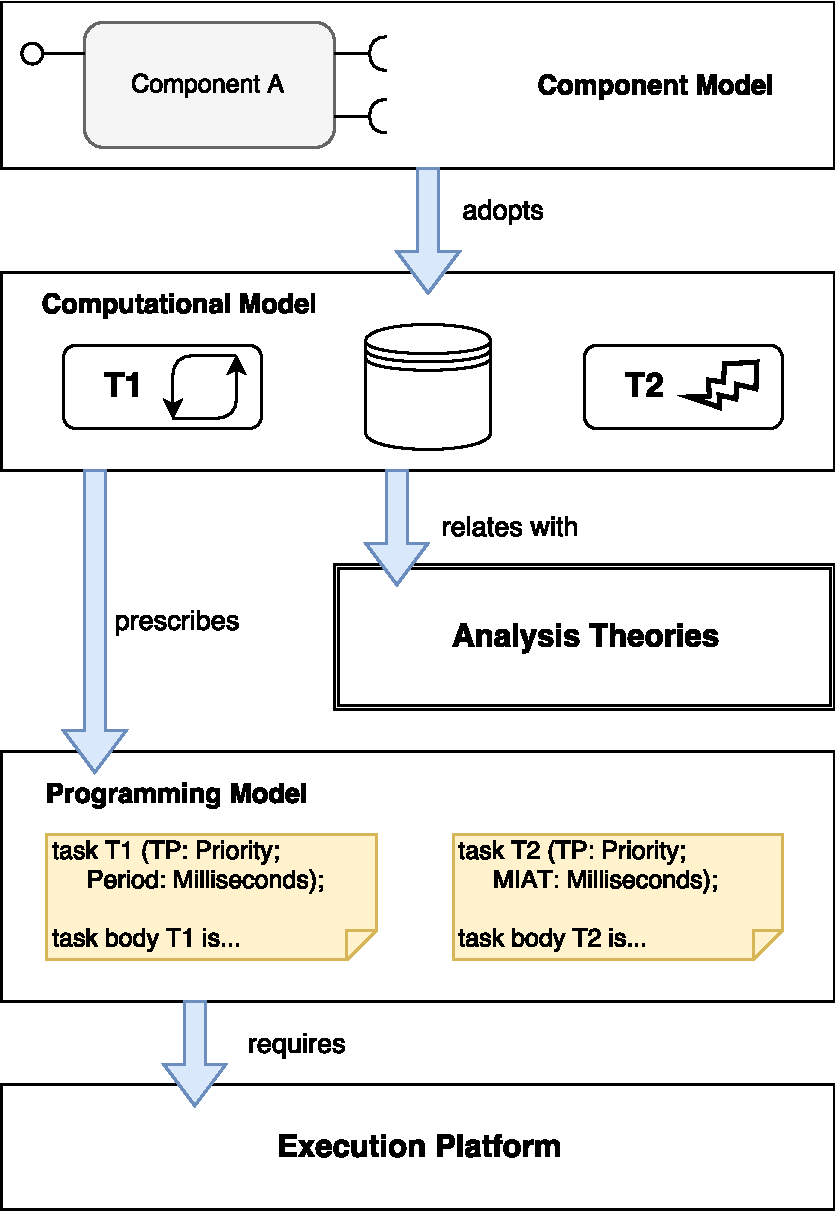
\includegraphics[width=0.5\textwidth]{ConstituentsOfSWArchitecture.pdf}
	\caption{The four constituents of the software reference architecture}
	\source{\cite{PhdThesis}}
	\label{fig: Constituents of OSRA}
\end{figure}

\subsection{Component Model}
\ac{cbse} is a software methodology centered on the systematic re-use of software by realizing the software as assembly of units of composition called components \cite{CBSE}.
The adoption of Component Based Software Engineering (CBSE) in the context of high-integrity real-time systems in general and in space domain in particular is not so popular as in the other main-stream domains like enterprise computing \cite{SAVOIR} because of strong verification and validation requirements imposed in the space domain and the presence of non-functional dimensions \cite{SAVOIR}.

The principles of Component Based Software Engineering (CBSE) when combined with the principles below can be used to build OBSW as an assembly of components \cite{SAVOIR}: 
\begin{itemize}
\item Principle of separation of concerns, by allocation of concerns to three distinct software entities: the component (which is a design entity), the container and the connector (which are entities used in implementation only and do not appear in the design space)
\item Possibility of verification of properties related to composability and compositionality \cite{CompBasedDev} 
\end{itemize}

The execution platform defined in the software architecture then provides the services to the components, container and the connectors. Finally, the entire software is deployed on the physical architecture (Computational units, equipment, and the network interconnections between them).

\subsubsection{\textbf{Founding principles of choice}}
This section describes the founding principles of choice of the component model:

\begin{description}
\item[Correctness by construction] E.W. Dijkstra in his ACM Turing lecture in 1972 suggested that the program construction should be done after a valid proof of correctness of construction has been developed \cite{CompBasedProcess}. Two decades later, a software development approach called Correctness by Construction (C-by-C) was proposed which advocated the detection and removal of errors at early stages, which leads to safer, cheaper and more reliable software \cite{CompBasedProcess}\cite{PhdThesis}. The Correctness by Construction practice follows:
\begin{itemize}
\item To give a solid reasoning on the correctness of the document or code, it is necessary to use formal and precise tools and notations for their development and verification 
\item Defining things only once so as to avoid contradictions and repetitions
\item Designing the software that is easy to verify e.g. by using safer language subsets or using appropriate coding styles and software design patterns. 
\end{itemize}

In OSRA and the component model developed along with it, the Correctness by Construction principle is changed to be applicable to a CBSE approach based on Model-driven Engineering (MDE) \cite{CompBasedProcess} wherein:

\begin{itemize}
\item The components are designed
\item The products designed by the design environment can be verified and analyzed by the design environment.
\item The lower level artifacts are automatically generated and the software production is automated to the maximum extent.  
\end{itemize}

\item [Separation of concerns] 
\label{section: Founding principle-Separation of concerns} 
Separation of concerns was first advocated by Dijkstra \cite{CompBasedProcess} and it helps to separate the aspects of software design and implementation. The OSRA and its associated component model promotes separation of concerns\cite{CompBasedProcess}\cite{PhdThesis}:

\begin{itemize}
\item The components are restricted to hold the functional code only. The non-functional requirements which has effects on the run-time behavior e.g. tasking, synchronization and timing are dealt by the component infrastructure, which is external to the component which realizes the functional code. The component infrastructure mainly consists of containers, connectors and their run-time support.

\item A specific annotation language is specified which is used to define the non-functional requirements and these are annotated on the components realizing the functional code.

By this, model transformations that automatically produce the containers and connectors that serve the non-functional requirements, enable the execution of the schedulability analysis directly on the model of components. This makes the implementation of the non-functional concerns fully compliant with its specification \cite{ScheduAnaly}. 

\item A code generator (whose development is the prime concern of this Master thesis) operates in the back-end of the component model, builds all of the component infrastructure that embeds the user components, their assemblies and the component services that help satisfy the non-functional properties \cite{CharEvoRAVCodeAr}. 
\end{itemize}

Inculcating the principle of separation of concerns in the development process has two major benefits \cite{CompBasedProcess}:

\begin{itemize}
\item It increases the reuse potential of the components, which is an important high level requirement described in the previous section \cite{SAVOIR}. The reuse potential of the component is increased because the same component can now be used under different non-functional requirements (as per the instantiations of the component infrastructure).

\item It helps in the generation of vast amount of complex and delicate infrastructural code which takes care of realizing the non-functional requirements on the run-time behavior of the software. This increases the readability, traceability and maintainability of the infrastructural code. 
\end{itemize}

\item [Composition] 
\label{section: Founding principle-Composition}
When composability and compositionality can be assured by static analysis, guaranteed through implementation, actively preserved at run-time, the goal of composition with guarantees as discussed by Vardanega can be achieved \cite{CompBasedProcess}. This is also one of the high level requirements defined in the section before.
 
Composability is guaranteed when the properties of individual components are preserved on component composition, deployment on target and execution. The components, as mentioned before, implement functional code, most part of which is sequential only and they do not have to worry about the non-functional semantics. The components behave like black-boxes and showcase to the external world only provided and required interfaces. Other components or infrastructural components are expected to communicate through these defined interfaces only. Hence, when components are composed with each other with matching required and provided interfaces, the functional composability is guaranteed which is necessary but not sufficient.

The non-functional requirements/constraints are annotated on the components (specifically the component interfaces) and they are realized by the container which encapsulates the respective component \cite{SAVOIR}\cite{ComponentModel}. The provided interface determines the semantics of the invocation and adds to the functional capabilities provided by the component. These semantics must match with the execution semantics described by the computational model, to which the component model is attached. An example for composable property is shown in \cref{fig: Composability}. In this case, the number of threads and protected objects generated per component, which entirely depends on the extra functional notations to the component interface should be invariant across component composition for the composable property to hold true.  

\begin{figure}[h]
	\centering
	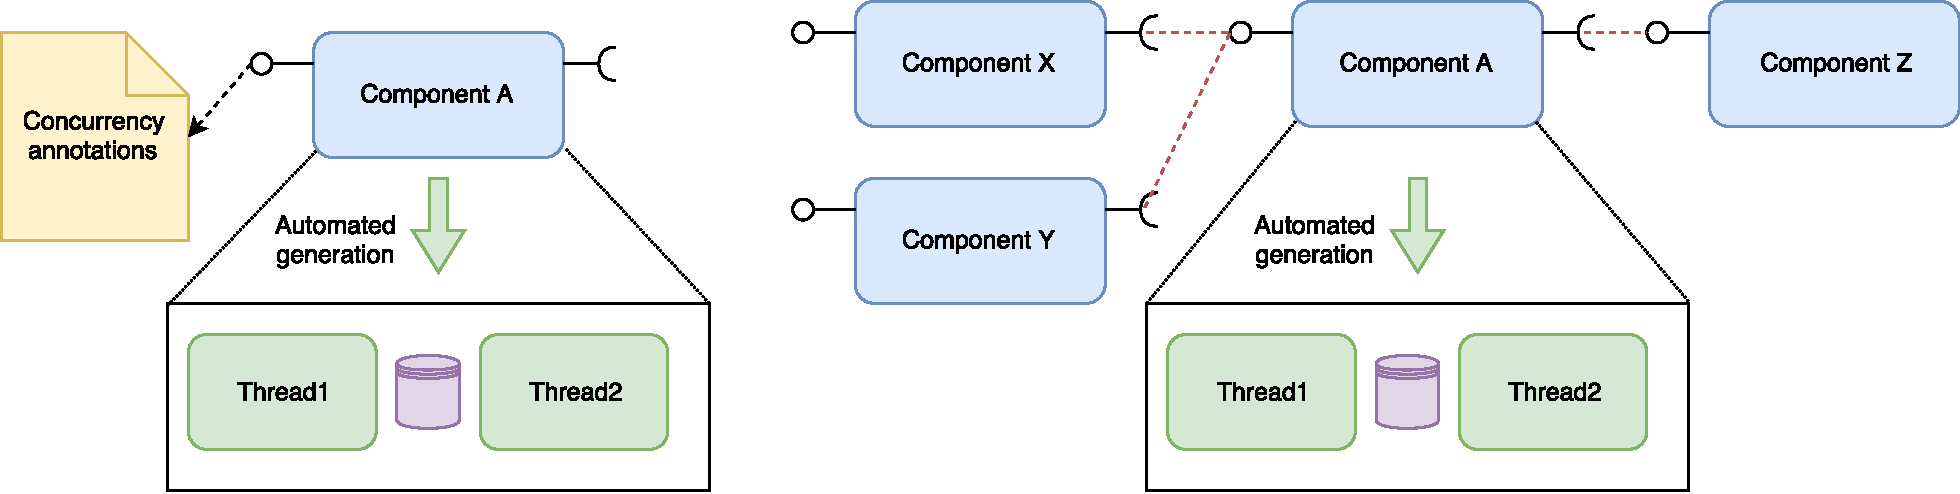
\includegraphics[width=1.0\textwidth]{Composability.pdf}
	\caption{Example for composability}
	\source{\cite{PhdThesis}}
	\label{fig: Composability}
\end{figure}

The computational model chosen should help extend composability to the non-functional constraints e.g. concurrency and the ones related to real-time and make it possible to get a compositional view of how execution occurs at the system level. Compositionality is said to be achieved when the properties of the system as a whole is a function of the properties of the constituting components. Finally, the binding of the computational model to the component should allow the execution semantics of the components with non-functional descriptors to be completely understood. An example for compositionality in shown in \cref{fig: Compositionality}. In this case, it should be possible to calculate the overall latency for the delivery of an output (i.e., the worst-case response time of the end-to-end chain of activities) from individual latencies of different components for the property of compositionality to hold true.

\begin{figure}[h]
	\centering
	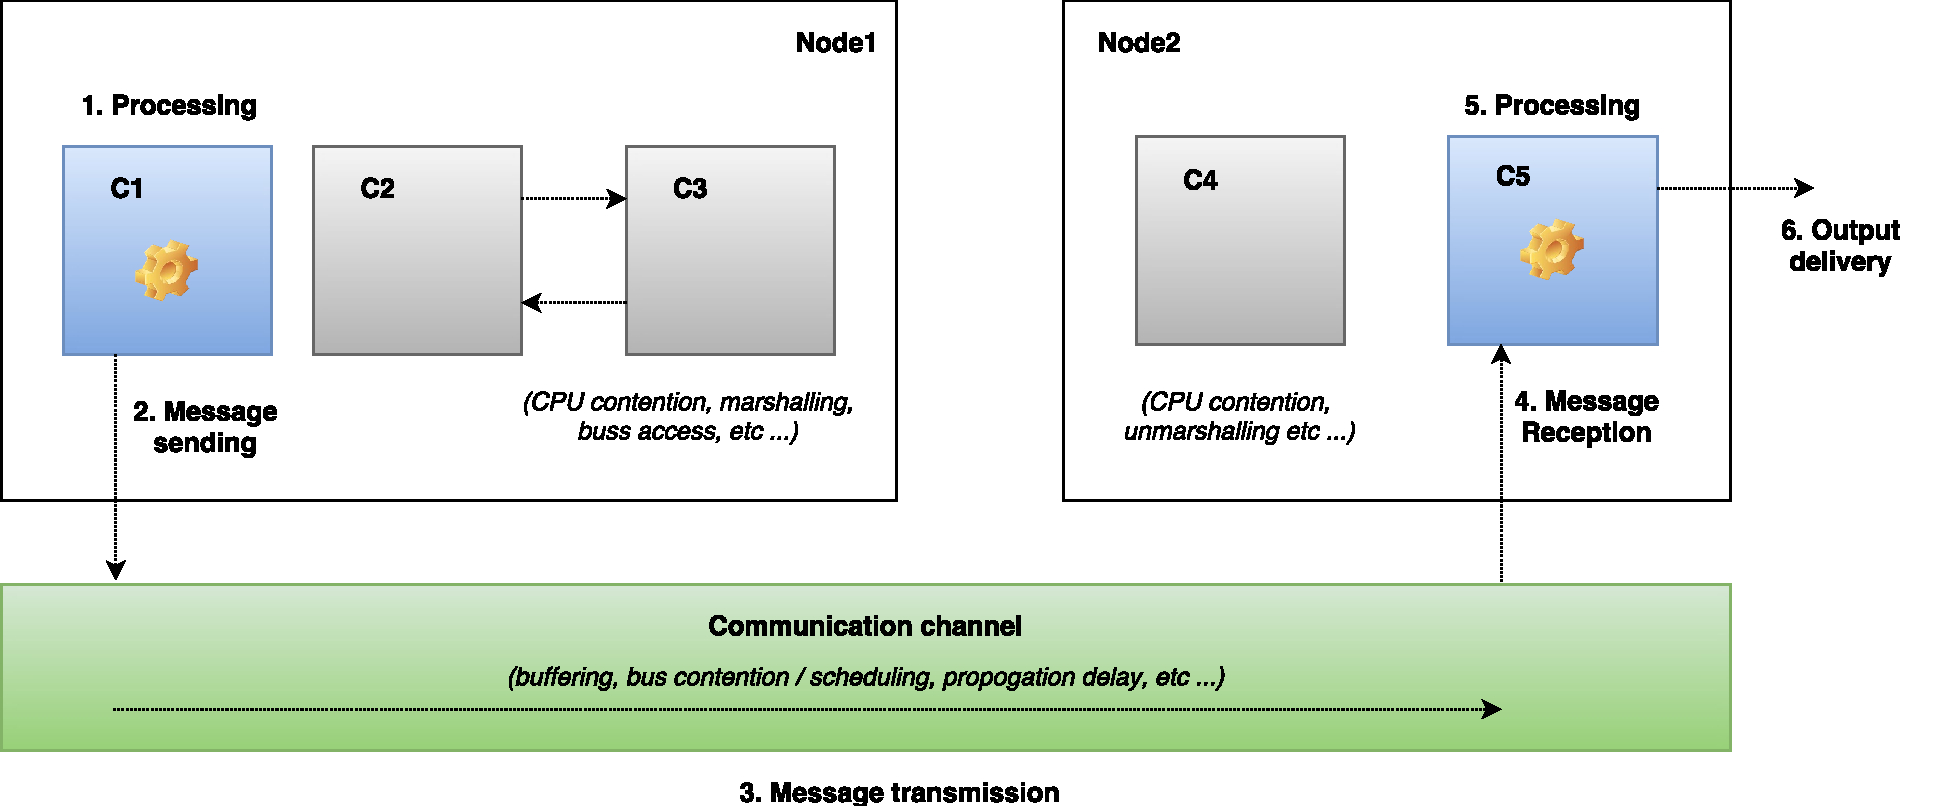
\includegraphics[width=1.0\textwidth]{Compositionality.pdf}
	\caption{Example for compositionality}
	\source{\cite{PhdThesis}}
	\label{fig: Compositionality}
\end{figure} 

In OSRA, the first and second needs can be met by having correct representations of the non-functional attributes in the component interfaces and the third need is taken care of by the generation of proper code artifacts, which is the main concern of this Master thesis.     
\end{description}

\subsubsection{\textbf{Software entities}}
\label {section: Software entities}
The following section describes more about components, containers and the connectors.

\begin{description}
\item[Component] Chaudron and Crnkovic describe that a Component model defines standards for properties that individual components must satisfy and the methods and possibly ways to compose components \cite{CompBasedProcess}.

A component provides a set of services and exposes them to the external world as a "provided interface". The service which is needed from other components or the environment in general are declared in a "required interface". A particular component connects to other components in order to satisfy the needs of its required interfaces. An event based communication system is also possible between components and a component can register to an "event service" to get notified about events emitted by other components.

Non functional attributes are added to the component interfaces as discussed before in the previous section on separation of concerns.

The adoption of hierarchical decomposition of components can be an effective way of defining components instead of defining a containment relationships. A child component can be developed to any component which would delegate and subsume the relationships between the interfaces of the child component and its parent. But the drawback is that various non-functional dimensions applicable to the space domain complicate the picture and hence is hierarchical decomposition of components not allowed at the current stage pf development \cite{PhdThesis}.
    
\item [Container] The container is a software entity that wraps around the component, which is directly responsible for realizing the non-functional properties. The relation between the component and the container is a famous software design pattern called the "inversion of control" \cite{CompBasedProcess}\cite{InvOfCntrlurl}. All in all, the reusable code (the container), controls the execution of the problem-specific code (the component).

The container exposes the same provided and required interfaces as that of the component and is able to support the component's execution with the desired, relevant non functional concerns attached to the component interface \cite{CompBasedDev}. The container also intercepts the calls made by the component to the other components/services requested from the target platform and transparently forward them to the container of the target component/target platform pseudo component (A pseudo component is a kind of component which is used for interaction purposes only). The former principle is called interface "promotion" and the latter is called the interface "subsumption" \cite{CompBasedDev}. The container and the component interact with each other according to the inversion of control design pattern, but the binding between components are still defined at software initialization time.

\item [Connector] The connector is a software entity responsible for the interaction between the components (actually between the containers that wrap around them). Connectors assist in implementing separation of concerns as the concerns of interaction is separated from the functional concerns. Components are thus void of code related to interactions with other components, however the the component model requires that the user specifies the interaction style in the component interfaces.

The component can be specified independently of the components it eventually binds to, the cardinality of the communication and the location of the other components it connects to, thanks to the principle of separation of concerns. 

No complex connectors are necessary in this Master thesis because, a simple linux based PC is chosen as a target system for component deployment and this greatly reduces the variety of connectors needed. Connectors necessary for function/procedure calls (which are usually straight-forward) are sufficient in this Master thesis. One of the major reasons, to go for a simple system is because this Master thesis does not deal with the hardware design or hardware modeling of the on-board software systems.           
\end{description} 

\cref{fig: Components containers and connectors} shows a connector mediating a connection between components A and B. The figure also shows components A and B being enveloped by their containers respectively. The containers would be responsible for the realization of the non-functional properties of the respective components they envelop. 

\begin{figure}[h]
	\centering
	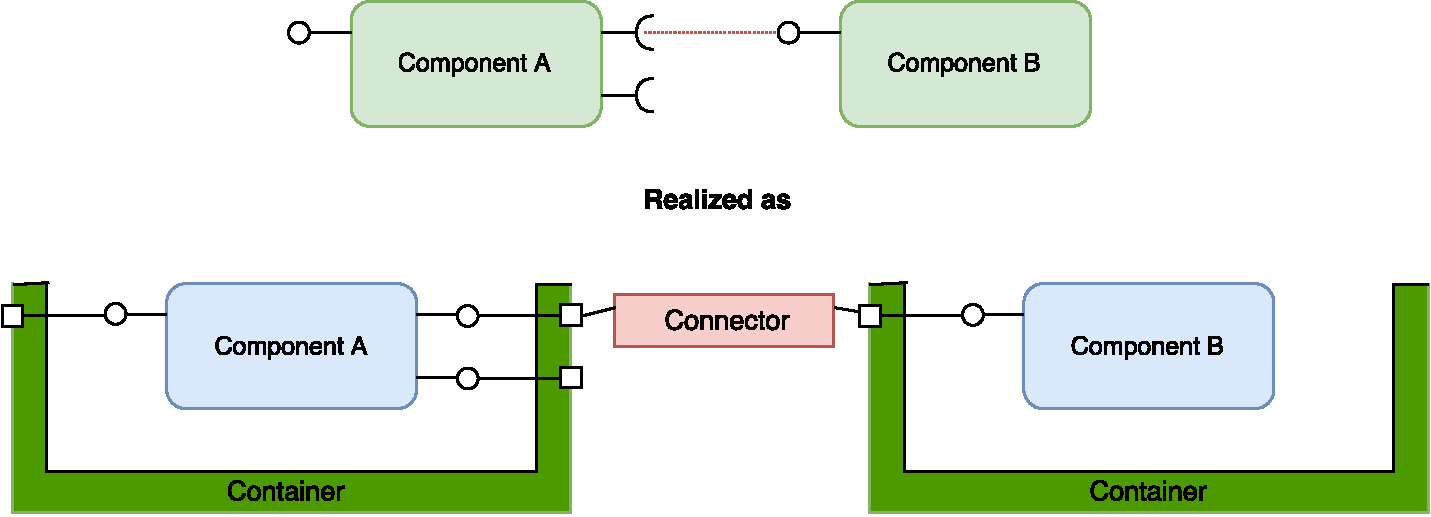
\includegraphics[width=0.8\textwidth]{ComponentContainerConnector.pdf}
	\caption{Components, containers and a connector connecting them}
	\source{\cite{SpecMetamodel}}
	\label{fig: Components containers and connectors}
\end{figure} 

\subsection{Computational model}
\label{section: Computational model} 
Using a computational model is necessary as per the Space Software engineering standard (ECSS-E-ST-440C) standard \cite{SAVOIR}. A dynamic software architecture is described according to an analyzable computational model which infers that the model development is fully consistent with that which underpins the mathematical equations which are used to predict the schedulability behavior of the system \cite{ScheduAnaly}. The computational model is more concerned about entities that belong to the implementation model (eg. tasks, protected objects and semaphores). A more abstract level description of these entities should be provided so that \cite{SAVOIR}:

\begin{itemize}
\item Pollution of the user-models with entities that are more primitive and are of interest to the lower levels of abstraction, is avoided. This is in line with the principle of separation of concerns, which is one of the high-level requirements.

\item The abstract representations represent the entities and their semantics faithfully.

\item Correct transformation of the information set by the designer in the higher-level representation to entities recognized by the computational model is ensured. This is in line with the principle of property preservation, which is also one of the high level requirements. 
\end{itemize} 

\subsection{Programming model and the execution platform}
\label{section: Execution platform}
The execution platform is a part of the software architecture providing all the necessary means for the implementation of a component and the computational model. It comprises of the middleware, the \ac{rtos}/\ac{rtk}, communication drivers and the board support package (BSP) for a given hardware platform. The services provided by the execution platform can be categorized into four different types \cite{SAVOIR}:

\begin{description}
\item [Services for containers] These services are meant to be used by the containers e.g. Tasking primitives, synchronization primitives, primitives related to time and timers.

\item [Services for connectors] These services are intended to be used by the connectors and it consists of actual communication means between components, ways to handle physical distribution across processing units, libraries used for translating data codes.

\item [Services to components] These services are supposed to be used by the components which implement the functional constraints. Typical services include: provision of on-board time for time-stamps, context management and data recovery. Access to these services are intercepted by the container wrapped around the component (refer section \cref{section: Software entities})

\item [Services to implement "abstract components"] These services include PUS monitoring, OBCPs, hardware representation etc.
\end{description}

It is important to note that different implementation of containers and connectors are necessary for each execution platform of interest.

The programming model realizes a given computational model and together with a conforming execution platform, it is possible to achieve the following goals \cite{PhdThesis}:

\begin{itemize}
\item Ensure that the implementation fully conforms with the semantics prescribed by the computational model and those assumed by the analysis
\item Ensure that the contracts stipulated between the components are respected at run-time. This is in-line with the principle of property preservation which is one of the high level requirements.
\end{itemize} 

The achievement of those two goals would then warrant that the system represented for the analysis purposes is a faithful representation of its implementation and the results of the analysis performed on the system model would be a valid prediction of the system at run-time \cite{PhdThesis}.

The programming model, which is the subject of this Master thesis, is realized by adopting Tasking framework as a computational model whose concurrency semantics would conform to the analysis model.     

% !TeX spellcheck = en_US

\chapter{Overall component-based software development process}
\label{chap: Software development process}
\section{Introduction}
In this chapter the design and implementation steps for the component-based software engineering (CBSE) approach are elaborated. The software design process involves two main actors: the software architect who is responsible for the entire software and provides support at system-level to the customer, and the software supplier who is responsible for the development of part of the software \cite{CompBasedProcess}. The parts of the software supplied by the software suppliers are then integrated in the final integration step.

Most of the activities described below come under the responsibility of the software architect, but as soon as the component is defined, it can undergo a detailed design and code implementation. This may indicate some shortcomings and flaws in the design of the component, which might trigger a re-design, re-negotiation of the component definition. This often leads to an iterative/incremental development process \cite{ScheduAnaly}. Detailed design and implementation of components is usually done by the software developers or it may be subcontracted to third party software suppliers. 

\section{Design entities and design steps}
There are two kind of entities which are defined in OSRA: Design-level entities which are explicitly specified in the design space and require the skills of the user to use them, real-time architecture entities which are not explicitly represented in the design space, instead they are automatically generated by the code-generation engines. The automatic generation of containers and connectors are possible only upon the knowledge of the computation model and execution platform that are going to be adopted \cite{SAVOIR,CompBasedProcess}. As already mentioned in the previous chapter, this master thesis considers Tasking Framework as the computational model and a normal linux based machine as the execution platform.   

The following entities belong to the design space: Data types, events, interfaces, component types, component implementations, component instances, component bindings and the entities required for the description of the hardware topology and platforms. The following entities belong to the real-time architecture: containers and connectors.

The development process is clearly divided into different steps \cite{CompBasedProcess, PhdThesis,SAVOIR}:

\begin{description}
\item [Step 1: Definition of data types and events] Data types are the basic entities in the approach and they can be primitive types, enumerations, ranged or constrained types, arrays or composite types (like structs in C or record types in Ada). An event is used in the publish-subscribe communication paradigm and it is an asynchronous message passing scheme.

\item [Step 2: Definition of interfaces] A set of operations with one or more already typed parameters, each with a direction (\texttt{in, in out, out}) are grouped together to form an interface. The interface can also hold a set of interface attributes of an already defined data type. The interface attributes can have read-only or read-write accesses. From the list of interface attributes, set of \texttt{getter} and \texttt{setter} operations can be generated for the attribute access, in particular \texttt{getter} operations for attributes with \texttt{read} only access and \texttt{getter},\texttt{setter} operations for attributes with \texttt{read-write} access. 

\item [Step 3: Definition of component types] Component types form the basis of a reusable software asset \cite{CompBasedProcess}. The software architect defines the component type to provide the specification of the functions that the component of this type would implement. The component types are independent of each other and they can consist of:
\begin{itemize}
\item One or more provided interfaces, which list the services that the component of this type would provide
\item One or more required interfaces, which list the functional services that the component of this type would require in order to function correctly according to the functional specifications
\item A set of component type attributes of already defined data types that are local to the component cannot be accessed from outside.
\item Event emitter/receiver ports to raise or receive events
In order to specify the provided and required interfaces, the component type references the interfaces that were defined in Step 2. This helps in straight forward matching of the required and provided interfaces  
\end{itemize}

\item [Step 4: Definition of component implementations] The software architect now creates and refines a component implementation from the component type. The component implementation contains the functional code in the form of source code that implements all the services that the component is supposed to provide. It acts as a  black box and only its external interfaces are only that matter. It is also a subcontracting unit to the software supplier. 

A component type can have more than one implementation and all of these implementations contain only pure sequential code i.e. it is void of any tasking or timing constructs. Implementations can be developed in multiple languages such as Ada, C, C++ etc.  

The component implementation should also provide constructs to store the attributes exposed through its provided interfaces and its component type. Technical budgets such as worst-case execution time (WCET) for a particular operation, maximum memory foot-print for component implementation, maximum number of calls to a certain operation on a required interface, can be placed on the entire component or on the operations and the implementation of the component shall respect this budget. Component implementation is thus a particularly attractive unit to be subcontracted to a third-party software supplier because the software architect can define components, attach technical budgets to it and delegate the implementation to he software suppliers. The software suppliers might add additional operations to the component implementation as and when necessary for the implementation \cite{CompBasedProcess}.  

\item [Step 5: Definition of component instances] A component instance is an instance of a component implementation. It is a deployment unit which is subjected to allocation on a processing unit and it is an entity on which the non-functional properties are specified. Specifically, the non-functional properties are attached to the provided interface side of the component, as they are the expression of a property or a provision of the component instance.

\item [Step 6: Definition of component bindings] Component bindings, as the name suggests, are the connections between one required interface of a component and the provided interface of another component. These bindings are set at design time and is subjected to static type matching to ensure that correct required and provided interfaces are connected to one another. This can be done by asserting the compatibility of the two interfaces (by type system or by inspection of the signature of their operations). If the binding is legal then whenever a call is made to an operation in the required interface, the call is dispatched to the correct operation in the bound provided interface. The signature of the calling operation in the RI (required interface) and the called operation in the PI (provided interface) are different and the connector, connecting these two interfaces, is in charge of performing this step. A tool support (possibly a back-end code generator) should initiate the configuration of the connector to perform this kind of binding.

It is also possible in this step to define bindings between an event emitter port of one component and an event receiver port of another component.

\item [Step 7: Specification of non-functional attributes] After component instances and component bindings have been defined, the software architect adds non-functional attributes to the services of the provided interfaces. 

In this step, the software architect specifies the timing and the synchronization attributes \cite{CompBasedProcess}. At first, the concurrency kind of the operation is established, and they can be \texttt{synchronous} or \texttt{asynchronous} operations. In case of a \texttt{synchronous} operation, it is executed in the flow of control of the caller and in case of an \texttt{asynchronous} operation, the operation is executed by a dedicated flow of control on the side of the callee. 

An \texttt{immediate} operation is said to be \texttt{protected} if it needs to be protected from data races in case of concurrent calls. The operation is said to be \texttt{unprotected} if it is free from such risks. In case of a \texttt{deferred} operation type, the architect can choose one of the following release patterns for the operation:

\begin{description}
\item [Periodic operation] The execution platform executes the operation at fixed periods with a dedicated flow of control.
\item [Sporadic operation] Two subsequent execution requests are separated by a minimum timespan called the minimum inter-arrival time (MIAT). The execution platform and the infrastructural code should guarantee this MIAT separation between two subsequent calls to the operation and the component implementer does not have to worry about it.
\item [Bursty operation] Only particular number of activations of an operation is allowed in a bounded interval of time. Again the execution platform and the infrastructure code guarantees this and the component implementer does not have to worry about it, as in the case for sporadic operation.
\end{description}

For all the operations which have concurrency kind set as \texttt{asynchronous}, the software architect must provide the worst case execution time (WCET) of the operation. A preliminary value of WCET is initially provided based on previous use of operations in other projects (if any) and they can be refined with bounds at later stages after performing a timing analysis for a given target platform.

\item [Step 8: Definition of physical architecture] The hardware topology provides a description of the system hardware limited to the aspects related to communication, analysis and code generation. It also provides a model-level description of the relevant hardware of the system. In the hardware topology, following elements are described:
\begin{itemize}
\item Processing units that have a general-purpose processing capability
\item Avionics Equipment/Instruments/Remote terminals
\item The interconnection between the elements mentioned above 
\item A representation of the ground segment/other satellites (eg. Formation flying) to state the connection between the satellite and ground segment or other space segments
\end{itemize}		
For the specification of these elements, following attributes are used:
\begin{description}
\item [Processor frequency] This is used for processors to re-scale WCET values expressed in processor cycles in Step 6
\item [Bandwidth] This is used for buses and point-to-point links and it indicates maximum blocking time due to non-preemptability of the lower priority message transmission (for whatever reason), minimum and maximum size of packets, minimum and maximum propagation delay, the maximum time that the bus arbiter/driver needs to prepare and send a message on the physical channel and maximum time for the message to reach the receiver    
\end{description}

\item [Step 9: Component instances and component bindings deployment] In this step, the component instances are allocated on the processing units defined in the hardware topology (refer Step 8). In majority of the cases, it is straight-forward to allocate the bindings between the components as they are deployed on the same processing units \cite{CompBasedProcess}. In other cases, they need to be specifically allocated.

\item [Step 10: Model-based analysis] The system model developed within the software reference architecture is subjected to schedulability analysis to determine whether the timing requirements set in the interfaces can be met.

From the user model which is a PIM (Platform Independent Model), a Schedulability Analysis Model (SAM) which is a PSM (Platform Specific Model) is created. This model is subjected to analysis and the results of the analysis is available for the software architect as a read-only result. 

The analysis transformation chain requires a model representation of the generated containers and connectors to be defined in the SAM for an accurate analysis \cite{CompBasedProcess}.

Please note that, step 10 is not of concern in this Master thesis as this Master thesis deals only with automatic generation of containers and connectors and hence an accurate model based schedulability analysis is outside the scope. Steps 8-9 are not of concern in this Master thesis, as it deals with hardware modeling and they are again outside the current scope of this Master thesis. However, these steps were mentioned for the sake of clarity and continuity.

\item [Step 11: Generation of containers and connectors]  This step is one of the main focus points of this Master thesis as mentioned before. Containers and connectors are generated and they specify:
\begin{itemize}
\item The structure of each container in terms of the required and provided interfaces of the enclosed component that they delegate and subsume
\item The structure of each connector 
\end{itemize} 
The non-functional attributes and the component instance and component connector deployment play a major role in determining the creation of connectors and containers and how component instances and their operations are allocated to them.

Concurrency can be achieved by encapsulating sequential procedures into tasks which reside in containers and the protection from concurrent accesses can be provided by attaching them concurrency control structures. All of this can be achieved without modifying he sequential code and simply by following the use relations among the components.

In order for the OBSW to interact with the external world, sensors and actuators need to be provided. These hardware entities are represented as pseudo components (A pseudo-component indicates that a component is for interaction purposes only) and software capability is attached to these components at the component instance level.    
\end{description}

\section{Design flow and design views}
\label{section: Design flow and views}
When the component model is defined, it also defines implicitly a design flow, that needs to be followed, to be able to create an OBSW that meet all its user needs and high level requirements \cite{SAVOIR, PhdThesis, CompBasedProcess}. The design flow is as explained in the previous section. 

The Obeo Designer Framework provides a concept called 'Viewpoint' and using this concept, the design views are implemented \cite{CompBasedProcess}. One of the advantages of the design views is to promote or enforce a certain design flow \cite{CompBasedProcess}. The component model is accompanied by the following design views:
\begin{description}
\item [Data view] This view is for the description of data types and events
\item [Component view] For definition of interfaces, components and the binding between them to fulfill their required needs
\item [Hardware view] For the specification of the hardware and the network topology
\item [Deployment view] For the allocation of components to computational nodes
\item [Non-functional view] In this view, the non-functional attributes are attached to the functional description of components
\item [Space-specific view] In this view, the services related to the commandability and observability of the spacecraft are specified
\end{description}  

\section{Language units of the OSRA}
\label{Language units}
The modeling language provided to the software architect to model the OBSW is divided for the ease of construction of the OBSW models into a set of language units \cite{SpecMetamodel}. Each language unit consists of closely related metamodel entities. OSRA Component model is composed of the following language units:

\begin{description}
\item [\texttt{CommonKernel}] Defines the basic entities that are used as the base elements of the language architecture
\item [\texttt{DataTypes}] Defines all the possible data and the data types that can be used in an OBSW model
\item [\texttt{SCM Kernel}] Defines the infrastructural part of the Space Component Model (SCM) which can be considered as the language to express all the concerns expressed by an OBSW model
\item [\texttt{Component}] Defines a complete set of interfacing features (interfaces, events, datasets), component types implementations and interface ports
\item [\texttt{Non-functional properties}] Defines the non-functional properties that can be applied to the modeling entities and a new language called the Value Specification Language (VSL) to specify values characterized by the measurement units
\item [\texttt{Deployment}] Defines instantiation and deployment entities such as component instances, connection between them and their deployment on the hardware architecture
\item [\texttt{Monitor and Control (M\&C)}] Defines the means to specify the technical properties related to M\&C that shall be provided in the OBSW model
\item [\texttt{Hardware execution platform}] Defines entities related to the execution platform, Time Space Partitioning (TSP) and the hardware architecture   
\end{description}

\section{OSRA SCM Model Editor}
\label{OSRA editor} 
The toolset that the software architect can use to build OBSW models is organized as a set of Eclipse features and Eclipse plugins. 

The toolset is available as
\begin{itemize}
\item A pre-installed Eclipse (Eclipse Neon) for Windows 64-bit  
\item An update site which consists of a set of static files which can be placed locally, on a web-server or on a file-server. 
\end{itemize}
In the latter case, the software architect would have to use the Eclipse Update Manager to install the plugins \cite{OSRAEditor}. 

In line with the design flow and design views explained in section \cref{section: Design flow and views}, different OSRA diagrams can be created with the help of OSRA SCM Model editor namely:
\begin{description}
\item [Interfaces, Events and Datasets diagram] This is the first diagram of the OSRA activity and allows to define the data types, events, data sets and the interfaces that would be used by the components in the Component Types diagram.
\item [Component Types diagram] This is the second diagram of the OSRA activity and it allows to define the component types, device types, execution platform service types, partition proxy types, required ports whose implementation would be used by the component instance diagram
\item [Component Instance diagram] This is the third diagram of the OSRA activity and it allows to define the component instances, device instances, execution platform service instances, partition proxy instances, provided interface slots, data receiver slots and event receiver slots.
\item [Hardware diagram] This is the last diagram of the OSRA activity and it allows to define the hardware elements such as processor boards, mass memory units, devices, buses.
\end{description}

There are also tables which are provided for diagram elements (if applicable) and they are usually found as tabs in pop-up window associated with the group that the element belongs to. Tables are usually classical tables where rows represents an element and each column represent a potentially computed property of the element. Rows can also contain sub-rows recursively which represent the sub-elements and the software architect can collapse or expand these sub-elements as desired. More information and details about install requirements and procedure, usage of the OSRA editor can be found in the reference \cite{OSRAEditor}.    
    

  
% !TeX spellcheck = en_US

\chapter{Tasking Framework}
\label{chap: Tasking framework}
\section{Introduction}
Future unmanned space missions have a great demand on computing resources for the on-board data processing or for control algorithms. Also, future space missions are requested to achieve more and more challenging scientific goals \cite{PhdThesis}. Besides the pre-processing of scientific data to reduce the data amount for the downlink, it is also necessary to handle the control systems with optical sensors, which come into play, for example in extra terrestrial navigation and landing systems \cite{ATON}. Space missions like the Rosetta mission or the landing of the Mars rover Curiosity were based on pre-defined timed command lists to control the landing \cite{TaskFr}. Because of this and the uncertainty of propulsion and parachute maneuver, the amount of different landing targets with low risks were considerably reduced \cite{TaskFr}. But the interesting areas of planetary research might also include risky landing areas and hence an autonomous control is needed for the spacecraft to control the trajectory and there is also a need to integrate hazard avoiding algorithms \cite{ATON}. However, these algorithms have a huge demand for computing power \cite{TaskFr}. 

In TET-1 satellite mission (Technology demonstrator) and \ac{bird} missions, the estimator and predictor modules were computed in a fixed order and fixed time in the control-cycle \cite{TETBIRD}. The timing was a combination of sensor latency and an additional gap time to satisfy the availability of data for computation and this led to a scant timing problem for the control torque computation due to over-estimated static safe-gap times \cite{TETBIRD}\cite{TETtoEUCROPIS}. During the \ac{leop}, a timing violation in another bus application resulted in changing the the order of inter-dependent computations and corrupted data, which further resulted in an unexpected \ac{aocs} state \cite{TETBIRD}. \cref{fig: Tasking} A) depicts such a situation and it can be observed that \texttt{ea = E(A)} is calculated before \texttt{eb = E(B)}. 

Also, the current on-board systems for the space environment do not provide the needed computing power \cite{TaskFr}. The space systems offer several controller boards on the spacecraft, most of them dedicated to only one subsystem and often twice for cold and hot redundancy. Such designs usually raise the power consumption and increase budgets like the mass, envelop and cost \cite{TaskFr}. Hence a concept, which allows sharing of computing resources based on predefined configurations for different flight phases and fault scenarios is necessary \cite{TaskFr}. The Tasking framework is an incarnation of the Inversion of Control design pattern which is popular practice in lightweight container frameworks \cite{InvOfCntrlurl}. 

A Tasking Framework is hence developed where the timing behavior is changed. Instead of starting computations at a predefined time in the computation cycle, a computation is started whenever the required information is available. All information are stored in messages distributed by channels and the channels initiate the computation when all the defined conditions for the computation are met \cite{TETBIRD}\cite{TETtoEUCROPIS}. The timing which can be achieved with Tasking Framework is as shown in \cref{fig: Tasking} B).    

\begin{figure}[h]
	\centering
	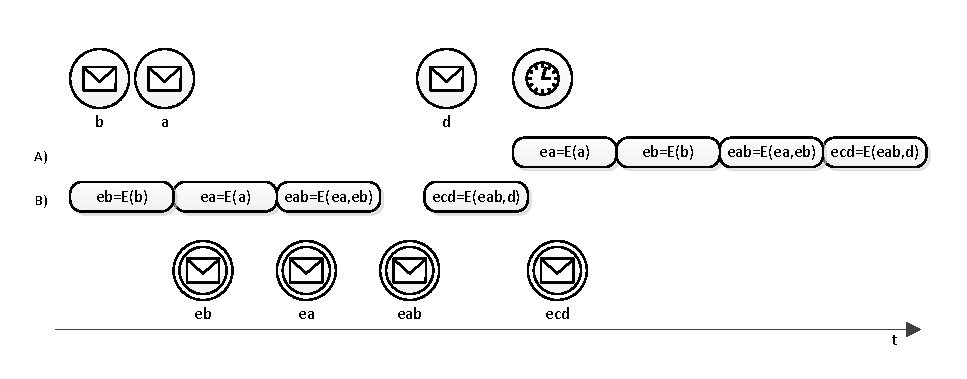
\includegraphics[width=0.8\textwidth]{TaskingFramework.pdf}
	\caption{Order and timing of computation tasks in BIRD and TET-1 vs order and timing of computation tasks in Eu:CROPIS}
	\source{\cite{TETtoEUCROPIS}}
	\label{fig: Tasking}
\end{figure}

\section{Usage of Tasking Framework}
The Tasking framework is based on C++ and provides some virtual base classes, which the application developer can overload to develop application specific computations. The Tasking Framework is designed to split the computations into small pieces, which are called tasks and they can be scheduled on the availability of the input data.

For each task, a number of task inputs can be specified and each input can be associated with a task channel which provides the memory space and the synchronization for messages consumed by the task. In order to start a task, the task input needs to be configured with the expected number of data pushes on the associated task channel and when the number of pushes on the task channel meets the expectation set, the respective task input is activated. When all the inputs of a particular task are activated, the task is automatically started by the scheduler of the Tasking Framework, provided a free computing core is available. If no computing core is available, then the task is queued for execution.

Any of the task inputs of a particular task can be marked as final and when such an input is activated, the respective task is started immediately by the scheduler irrespective of the activation states of the other task inputs. As a result, the task can push onto another channel, which can trigger the other task associated with this channel. This leads to a kind of behavior similar to petri nets \cite{Petrinet}, where the activation of the task input is a token and the task execution is a transition \cite{TaskFr}. The inputs associated to a task are reset when all its inputs are activated or when the respective activated input is marked as final. Such a reset operation on a task input sets the number of arrived data items on the associated task channel back to zero.

To specify timings in the Tasking framework, a special channel called 'event' is provided \cite{TaskFr}. An event is associated with a clock and the task input to which it is associated is notified on each clock tick. When the required number of notifications match the expected number which is already set, the attached task input is activated. A Task event can be configured to work with absolute timing, i.e. the associated task input and in-turn the task itself is activated at fixed points in time, or a task event can be configured to work with a relative timing i.e, the task input and in-turn the task is activated at points in time relative to the execution time of the task.

To support mapping of tasks in a distributed system, task channels are associated with interfaces to read and write from and to networks and devices. These associations are set up by the configuration manager and are not visible to the application developer \cite{TaskFr}.

The current implementation of Tasking framework sits on top of Linux \ac{posix} library, composed by a real-time clock interface, signaling mechanism, memory access and the tasks scheduler. The Tasking framework can also run on operating systems like \ac{rtems} and FreeRTOS using the outpost libraries which collectively provide a high level abstraction of the underlying operating system \cite{TaskFr}.

\section{Use cases for Tasking Framework}
In the project \ac{obc-ng} by \ac{dlr}, a decision was made to design the on-board computer systems as a combination of space qualified processing node, \ac{cots} processing nodes and network nodes \cite{TaskFr}. As an operating system for this project, an enhancement of \ac{rodos} was used \cite{TaskFr}\cite{OBC-NG}. The enhancement covered mainly the support for multi-core and reconfigurable distributed systems \cite{RODOS} and the core element which made it possible was the Tasking Framework \cite{TaskFr}. The configuration manager used in OBC-NG held predefined mappings of tasks and resources for different hardware configurations of computing resources and mission phases \cite{OBC-NG}. The communication infrastructure was set up based on the mappings during the configuration phases of the system. 

The first usage of the Tasking framework was in the \ac{aton} project \cite{ATON}. The project was about the navigation system for a moon landing scenario. The project showed that the Tasking framework was a useful way for the parallelization of computations in an expected manner \cite{ATON}.

Another use-case of Tasking Framework is in the AOCS of \ac{eucropis} mission \cite{TETtoEUCROPIS}. Eu:CROPIS uses a porting of the Tasking framework from Linux to outpost libraries which collectively act as an operating system \ac{api} on top of RTEMS \cite{TETtoEUCROPIS}.

Tasking framework is also used in project named \ac{maius} which deals with activities to demonstrate Bose-Einstein condensation and atom interferometry with rubidium and potassium atoms on a sounding rocket \cite{TETtoEUCROPIS}\cite{MAIUS}.

\section{Use of Tasking Framework in this Master thesis}
\label{section: Use of tasking}
Tasking framework is used as a computational model, as discussed in the previous chapter. The reasons for adopting Tasking Framework in this Master thesis are the following:

\begin{itemize}
\item The Tasking framework guarantees that the timing behavior of the system is deterministic and amenable to static analysis.
\item The Tasking framework has been proven to be expressive enough to handle real-world application as discussed in the previous section.
\item Tasks do not interact with each other directly, but their communications are mediated by protected objects (task channels). These channels are shared resources equipped with a synchronization protocol in the form of priority based scheduling and \ac{fifo} scheduling for tasks with same priorities which uses these shared resources \cite{TaskFr}.  
\end{itemize}  

However, during the course of this Master thesis, certain short-comings of Tasking framework have however been identified and can be found in \cref{section: Identififed shortcomings} of \cref{chap:conclusion}.

             



          
% !TeX spellcheck = en_US

\chapter{Infrastructural code generation}
\label{chap: Code generation}
\section{Introduction}
After designing an OBSW model using the OSRA SCM model editor and following the component-based software development approach that comes with it, the OBSW model entities need to be mapped to the infrastructure code. The reference programming model for OSRA, discussed in the previous chapter helps us in progressing towards this goal. But, it is necessary to understand the overall design approach for the generated code and briefly present the abstractions that will be offered to the software supplier. This chapter, deals with these things in detail. Similar efforts from the Artemis JU CHESS project \cite{EvoRAVCodeAr}, provide the perfect base for discussions in this chapter of the Master thesis.   

\section{User model entities in the Platform Independent Model (PIM) phase}
A detailed description of all the modeling entities that the software architect can use, can be found in the specification of the metamodel for the OSRA component model \cite{SpecMetamodel}. However a brief description of them is noteworthy here:
 
\begin{description}
\item [Datatypes] The software architect can create a set of project-specific data types and constants using the \texttt{Data Types} language unit of the \texttt{CommonTypes} metamodel and the language unit is designed to provide the software architect an expressive power comparable to the languages with strong types (e.g. Ada).\cite{SpecMetamodel}. The supported type definitions are boolean types, integer types, float types, enumeration types, fixed point types, array types, structured types, string types, union types, alias types, opaque types, external types and unconstrained types. Some of these data type definitions are obvious for readers with programming skills in typed languages such as Ada, C or C++. 

\item [Interface] An interface is a specification of coherent set of services and it represents the definition of a contract. An interface is defined independently of the entities implementing it (e.g. Component type). An interface may enlist declaration of operations, which are the functional services that shall be offered by the entities implementing it. The services include a name, set of ordered parameters and one or more exceptions that they might throw when things go wrong during the handling of the service. Parameters are typed with one of the types mentioned above and have a mode (\texttt{in, out} or \texttt{inout}). A component type may expose one or more interfaces and the same interface can be exposed by different component types. An interface may also contain the declaration of one or more interface attributes, which are the parameters that are accessible via the interface implementations.

\item [Component type] A component type is an entity which specifies the external interfaces of a software component and are defined in isolation and are used to declare relationships with the other components and system in general. It conforms to the principle of encapsulation and as a consequence, all the interactions with other components are performed exclusively via its explicitly declared interface. A component type usually encompasses:
\begin{itemize}
\item A list of provided interface ports
\item A list of required interface ports
\item A list of dataset emitter ports 
\item A list of dataset receiver ports
\item A list of event emitter ports
\item A list of event receiver ports 
\end{itemize}

\item [Component implementation] It is an entity that represents a concrete realization of a component type. It is functionally identical to the component type except that the source code is added to the component implementation and may also define number of component implementation attributes

\item [Component instance] It is an instantiation of a component implementation and hence contains all the instantiations of the structural features, such as provided and required interface ports. It also contains instantiation of all attributes (interface attributes, component type attributes and component implementation attributes). It is also the elementary deployment unit for the OBSW model \cite{SpecMetamodel}.        
\end{description}

\section{Mapping of design entities to the infrastructural code}
As the generated code should target the Tasking framework, which is the target computational model in this Master thesis and because the Tasking framework is written in C++, the following sections explains the mapping of design entities to the infrastructure code that will be generated in C++.

On analyzing the specifications of the metamodel for the OSRA component model \cite{SpecMetamodel}, it is clear that there are different corner cases that can arise during the construction of the OBSW models using OSRA component model and it is necessary that these corner cases are effectively handled in the software design for the infrastructural code. The following sections try to build an OBSW model keeping the the corners cases in mind and attempt to explain the overall design approach.

\subsection{Corner cases arising during the construction of OBSW model using OSRA component model}
The different corner cases which can arise are:

\begin{itemize}
\item Multiple provided interfaces which refer to the same interface type are promoted by the container of a component
\item Multiple required interfaces which refer to the same interface type are subsumed by the container of a component
\item Multiple interfaces provide exact same operations
\item Multiple implementations per component type
\end{itemize}

The first and second corner cases are handled in the following example. But, the other cases will be treated directly in the later section, which deals with the software design for the generated infrastructure code. 

\subsection{An example OBSW model}
Our simple OBSW model, yet effective to serve the intended purpose, is built as per the proposed component-based development approach explained in the section \cref{section: Design steps} in chapter \cref{chap: Software development process}. As already mentioned in that section, the component-based approach puts a lot of emphasis on the definition of component interfaces \cite{CompBasedProcess} and it is followed here as well. Components are built from scratch using newly defined interfaces. All model entities defined here are instantiations of the modeling entities specified in the metamodel \cite{SpecMetamodel}. The OBSW model is designed using the OSRA SCM model editor mentioned in the section \cref{section: OSRA editor} in chapter \cref{chap: Software development process}. The model entities from the OSRA SCM model editor can be exported as images and they are used in this sub-section for illustration purposes.

In this simple example, two simple components are designed. The first component requests for a service \texttt{OperationAdd} which can add two numbers, as the name suggests and this service is implemented in the second component. Another service namely \texttt{Call\allowbreak Operation\allowbreak Add} is implemented in the first component, which can be requested to trigger the OBSW model. Different non-functional properties, as explained later in this section, are strewn on the required and provided interfaces of these components to make example, a bit more interesting and also to capture the above mentioned first and second corner cases in the example.

\begin{description}
\item [Step 1: Definition of data types and events] As the Master thesis requires to emphasize more on effectively capturing interactions and concurrency semantics required for communication between the designed components, the data types chosen in this example are fairly simple. But it is important to note that the scheme of mapping of these simple data types to the infrastructural code (explained in the later sections), can be scaled to fairly complex data types as well. The data types, exception types and the event type used in this example are as shown in \cref{fig: Ex. Datatypes etc.}  

\begin{itemize}
\item Two data types namely \texttt{Fixed\allowbreak Length\allowbreak String\allowbreak Type} and \texttt{Integer\allowbreak Type} of type \texttt{UNSIGNED} are defined and they are named as \texttt{StringType} and \texttt{IntegerType} respectively

\item Three exception types, named as \texttt{OperandException}, \texttt{MemoryException} and \texttt{Overflow\allowbreak Exception} are defined 

\item An \texttt{Event} type, which can be used for asynchronous notifications \cite{SpecMetamodel} is instantiated and it is named as \texttt{FailureEvent}. Two event parameters are also instantiated as shown in \cref{fig: Ex. Datatypes etc.}

\end{itemize} 

\item [Step 2: Definition of interfaces] Two interface namely \texttt{InterfaceA} and \texttt{InterfaceB} are designed as shown in \cref{fig: Ex. Datatypes etc.}. \texttt{InterfaceA} has only one single operation by name \texttt{CallOperationAdd} and \texttt{InterfaceB} has an operation by name \texttt{OperationAdd} and an interface attribute of data type \texttt{IntegerType} and named as \texttt{m\_StatusValue}.  

\begin{itemize}
\item The operation \texttt{Call\allowbreak OperationAdd} is a parameterless operation and it is intended to be the service which can in turn request the service which can add two numbers.

\item The operation \texttt{OperationAdd} in \texttt{InterfaceB}, as the name suggests, is intended to be the service which can add two numbers, send back the results and raise a pre-defined exception if necessary. It has three operation parameters and can throw different exceptions as mentioned in \cref{fig: Ex. Datatypes etc.}. 

\item The interface attribute \texttt{StatusValue} in \texttt{InterfaceB} is of type \texttt{CFG} and it indicates that the interface attribute is a configurable parameter \cite{SpecMetamodel}. As a result, two operations for the purpose of setting and getting the values of the interface attribute are defined.      
\end{itemize}

\begin{figure}[h]
	\centering
	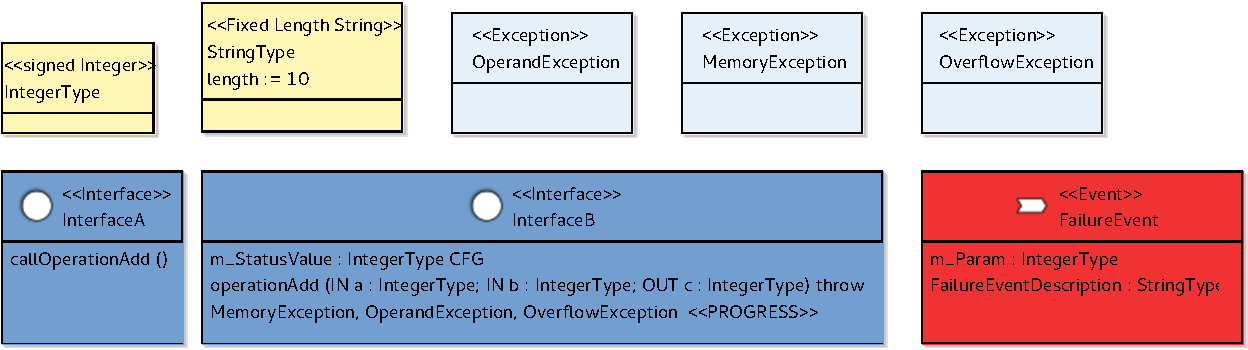
\includegraphics[width=1.0\textwidth]{InterfacesEventsDatasetsDiagram.pdf}
	\caption{Data types, events, exceptions and interfaces diagram}
	\label{fig: Ex. Datatypes etc.}
\end{figure}

\item [Step 3: Definition of component types] Component types namely \texttt{Component\allowbreak\_Caller} and \texttt{Component\allowbreak\_Callee} which form the basis for a reusable software asset are defined as shown in the \cref{fig: Ex. Component types}. 

\texttt{Component\allowbreak\_Caller} has:
\begin{itemize}
\item Provided interface port \texttt{Provided\allowbreak Interface\allowbreak Port} which refers to \texttt{InterfaceA}
\item Required interface port \texttt{Required\allowbreak Interface\allowbreak PortType1} which refers to \texttt{InterfaceB}
\item Required interface port \texttt{Required\allowbreak Interface\allowbreak PortType2} which refers to \texttt{InterfaceB}
\item Event receiver port \texttt{FailureEvent\allowbreak ReceiverPort} which refers to \texttt{Failure\allowbreak Event}
\end{itemize}

The desired interaction kind for the operations in the required interface ports of \texttt{Component\allowbreak\_Caller} are as shown in the \cref{table: NFP RI Ports}

\begin{table}[]
	\centering
	\caption{Desired interaction kind for operations in the required interface ports}
	\label{table: NFP RI Ports}
	\begin{tabular}{|c|c|c|}
		\hline
		\textbf{Required interface ports} & \textbf{Operations} & \textbf{Interaction kind} \\ \hline
		\texttt{RequiredInterfacePortType1} & \begin{tabular}[c]{@{}c@{}}\texttt{OperationAdd}\\ Interface attribute setter\\ Interface attribute getter\end{tabular} & \begin{tabular}[c]{@{}c@{}}\texttt{synchronous}\\ \texttt{synchronous}\\ \texttt{synchronous}\end{tabular} \\ \hline
		\texttt{RequiredInterfacePortType2} & \begin{tabular}[c]{@{}c@{}}\texttt{OperationAdd}\\ Interface attribute setter\\ Interface attribute getter\end{tabular} & \begin{tabular}[c]{@{}c@{}}\texttt{asynchronous}\\ \texttt{asynchronous}\\ \texttt{asynchronous}\end{tabular} \\ \hline
	\end{tabular}
\end{table}

\texttt{Component\allowbreak\_Callee} has:
\begin{itemize}
\item Provided interface port \texttt{Provided\allowbreak Interface\allowbreak Port1} which refers to \texttt{InterfaceB}
\item Provided interface port \texttt{Provided\allowbreak Interface\allowbreak Port2} which refers to \texttt{InterfaceB}
\item Event emitter port \texttt{FailureEvent\allowbreak EmitterPort} which refers to \texttt{FailureEvent}
\end{itemize}

\begin{figure}[h]
	\centering
	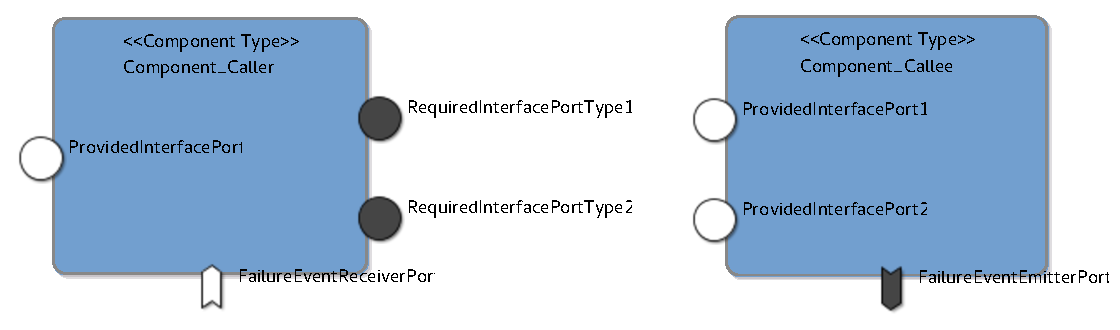
\includegraphics[width=1.0\textwidth]{ComponentTypesDiagram.pdf}
	\caption{Component types diagram}
	\label{fig: Ex. Component types}
\end{figure}

\item [Step 4: Definition of component implementations] Component implementations are created from the component types.

\texttt{Component\allowbreak\_Caller} has one component implementation named as \texttt{Component\allowbreak\_Caller\_impl} and \texttt{Component\allowbreak\_Callee} has one component implementation named as \texttt{Component\allowbreak\_Callee\_impl}. The component implementation \texttt{Component\allowbreak\_Callee\_impl} implements the means to store the attribute \texttt{Param} of \texttt{InterfaceB}, that is exposed through its provided interface ports, namely \texttt{Provided\allowbreak Interface\allowbreak Port1} and \texttt{Provided\allowbreak Interface\allowbreak Port2}.

No maximum memory footprint for component implementations are defined or no detailed design activity of the component implementations are performed as they are not of concern in this Master thesis.

\item [Step 5: Definition of component instances] The component instances are the instances of component implementations \cite{CompBasedProcess}.

Two component instances as shown in \cref{fig: Ex. Component instances} are defined, namely:
\begin{itemize}
\item \texttt{Component\allowbreak\_Caller\_impl\_inst} which is an instantiation of \texttt{Component\allowbreak\_Caller\_impl}
\item \texttt{Component\allowbreak\_Callee\_impl\_inst} which is an instantiation of \texttt{Component\allowbreak\_Callee\_impl}
\end{itemize}

\item [Step 6: Definition of component bindings] Component bindings as shown in \cref{fig: Ex. Component instances} are defined:

\begin{figure}[h]
	\centering
	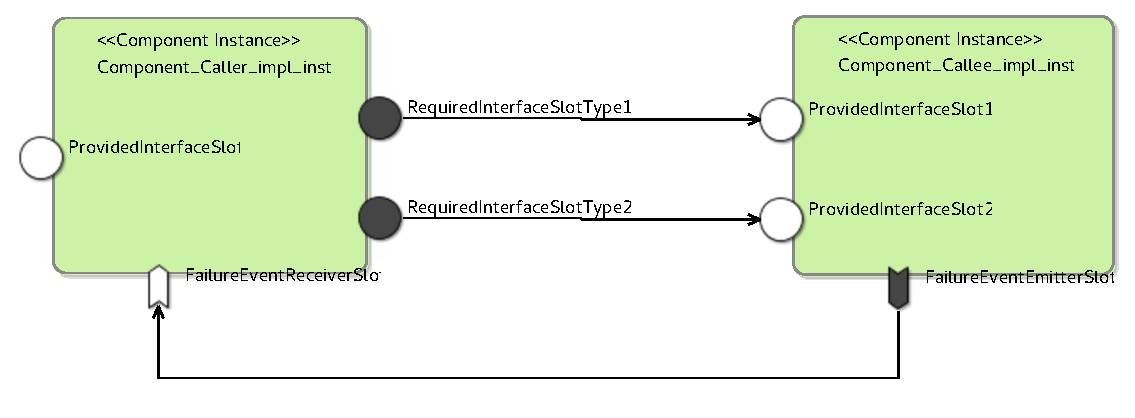
\includegraphics[width=1.0\textwidth]{ComponentInstancesDiagram.pdf}
	\caption{Component instances diagram}
	\label{fig: Ex. Component instances}
\end{figure}

\item [Step 7: Specification of non-functional attributes] The non-functional properties are defined on the component instances and the component bindings defined in the previous step. The non-functional properties language unit of the specification of a metamodel provides a Value Specification Language (VSL) unit, which permits the specification of the the non-functional properties qualified with a measurement unit \cite{SpecMetamodel}. The VSL is used here to define values of non-functional properties with a measurement unit.

For the provided interface slot in the component instance \texttt{Component\allowbreak\_caller\allowbreak\_impl\_inst}, the following non-functional property is specified as shown in \cref{table: NFP PI Ports1}

\begin{table}[]
	\centering
	\caption{Non-functional property for the operation in the provided interface slot}
	\label{table: NFP PI Ports1}
	\begin{tabular}{lll}
		\hline
		\multicolumn{1}{|c|}{\textbf{Provided interface slot}} & \multicolumn{1}{c|}{\textbf{Operation}} & \multicolumn{1}{c|}{\textbf{Non-functional property}} \\ \hline
		\multicolumn{1}{|c|}{\texttt{ProvidedInterfaceSlot}} & \multicolumn{1}{c|}{\texttt{CallOperationAdd}} & \multicolumn{1}{c|}{\texttt{cyclic}, Period = 2s} \\ \hline
	\end{tabular}
\end{table}

For the provided interface slots in the component instance \texttt{Component\allowbreak\_callee\_impl\_inst}, the following non-functional properties are specified as shown in \cref{table: NFP PI Ports2}

\begin{table}[]
	\centering
	\caption{Non-functional properties for the operations in the provided interface slots}
	\label{table: NFP PI Ports2}
	\begin{tabular}{ccc}
		\hline
		\multicolumn{1}{|c|}{\textbf{Provided interface slots}} & \multicolumn{1}{c|}{\textbf{Operations}} & \multicolumn{1}{c|}{\textbf{Non-functional properties}} \\ \hline
		\multicolumn{1}{|c|}{\texttt{ProvidedInterfaceSlot1}} & \multicolumn{1}{c|}{\begin{tabular}[c]{@{}c@{}}\texttt{OperationAdd}\\ Interface attribute setter\\ Interface attribute getter\end{tabular}} & \multicolumn{1}{c|}{\begin{tabular}[c]{@{}c@{}}\texttt{Protected}\\ \texttt{Protected}\\ \texttt{Unprotected}\end{tabular}} \\ \hline
		\multicolumn{1}{|c|}{\texttt{ProvidedInterfaceSlot2}} & \multicolumn{1}{c|}{\begin{tabular}[c]{@{}c@{}}\texttt{OperationAdd}\\ Interface attribute setter\\ Interface attribute getter\end{tabular}} & \multicolumn{1}{c|}{\begin{tabular}[c]{@{}c@{}}\texttt{Sporadic}, MIAT = 2s\\ \texttt{Protected}\\ \texttt{Protected}\end{tabular}} \\ \hline
		\multicolumn{1}{l}{} & \multicolumn{1}{l}{} & \multicolumn{1}{l}{}
	\end{tabular}
\end{table}

It is important to note that the WCET and deadline values for the operations in the provided interface slots are not handled, as the safeguarding of these properties are not of concern in this Master thesis.

For the event receiver slot in the component instance \texttt{Component\allowbreak\_caller\allowbreak\_impl\allowbreak\_inst}, the following non-functional property is specified as shown in \cref{table: NFP ER Port}

\begin{table}[]
	\centering
	\caption{Non-functional property for event reception}
	\label{table: NFP ER Port}
	\begin{tabular}{ccc}
		\hline
		\multicolumn{1}{|c|}{\textbf{Event receiver slot}} & \multicolumn{1}{c|}{\textbf{\texttt{Event}}} & \multicolumn{1}{c|}{\textbf{Non-functional property}} \\ \hline
		\multicolumn{1}{|c|}{\texttt{FailureEventReceiverSlot}} & \multicolumn{1}{c|}{\texttt{FailureEvent}} & \multicolumn{1}{c|}{\texttt{Protected}} \\ \hline
		\multicolumn{1}{l}{} & \multicolumn{1}{l}{} & \multicolumn{1}{l}{}
	\end{tabular}
\end{table}

\item [Step 8: Definition of the physical architecture] The hardware topology provides a description of the system hardware. As hardware modeling is not of concern in this Master thesis, a simple hardware topology as shown in \cref{fig: Ex. Hardware topology} is considered. 

A processor board with a processor and a processor core is instantiated. Two connection docks are attached to the processor board and a bus is used to connect the connection docks. The component instances are deployed on the processor core and the component bindings are deployed on the bus.

\begin{figure}[h]
	\centering
	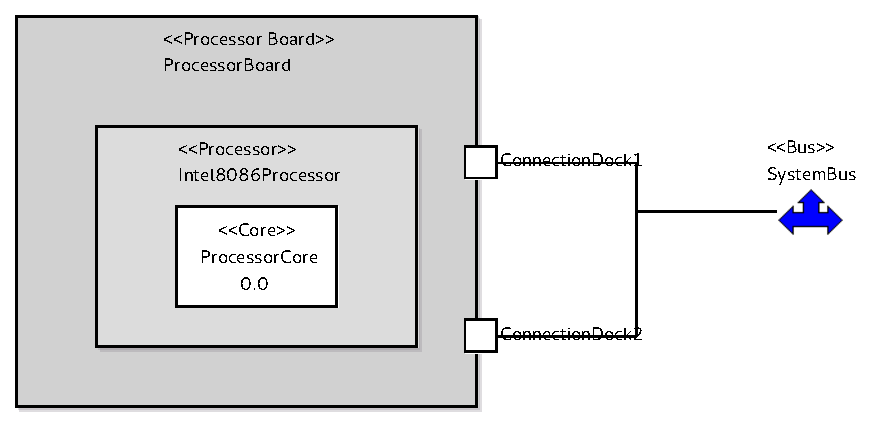
\includegraphics[width=0.8\textwidth]{HardwareDiagram.pdf}
	\caption{Hardware topology diagram}
	\label{fig: Ex. Hardware topology}
\end{figure}
 
\end{description}

This OBSW model is subjected to model validation against the OSRA Specification Compliance and the SCM meta-model compliance, in the OSRA SCM editor \cite{OSRAEditor}. Only after the OBSW model is successfully validated, can the OBSW model be considered as a suitable candidate for automatic generation of infrastructure code \cite{OSRAEditor}.  
   
\subsection{Software design approach for the generated code}
\label{subsection: Software design approach}
This section deals with the software design approach for the generated infrastructure code. Some of the necessary good characteristics of a software such as reusability, separation of concerns and minimal complexity are targeted already at the reference architecture level and it needs to be safeguarded at the generated software level as well. The other main characteristics of the generated software which are of utmost value are \cite{CodeComplete}:
\begin{description}
\item [Testability] The software must be testable and there must be suitable constructs in the generated software which assist in writing automated unit tests or user driven tests to test it. In this Master thesis, it is taken care that the generated C++ classes have corresponding abstract base classes, using which mock classes can be constructed easily for the purpose of testing. More about this is explained in the next chapter which focuses on further scope of this Master thesis
\item [Extensability and Refactorability] The software generated must be loosely coupled so that the entire code base is more resilient to changes and extensions. Dependency injection software design pattern \cite{InvOfCntrlurl} is used wherever appropriate to make the generated software loosely coupled
\item [Portability] The generated software must be portable across systems and environments. The data  types used in the generated software should be portable across multiple platforms and the data type standardizations from C++11 are made use of in the generated software
\item [High fan-in] The generated software is designed in a way that a particular C++ class is used by large number of other C++ classes.
\item [Low-to-medium fan-out] The generated software is designed in a way that a particular C++ class uses not many classes, so that the complexity of the generated software is not too high. Unfortunately, this characteristic is not completely respected in this software design, because the complexity of a particular class depends on the complexity of the user model.      
\end{description}
UML class diagrams, wherever appropriate are judiciously used in this section to show a high level representation of the generated C++ classes and datastructures. 

Each of the following sub-sections, is divided into two parts:
\begin{itemize}
\item The first part throws light on the idea of how a mapping of a given model entity to an infrastructural code entity can be done
\item The second part makes the approach clear by taking the reference of our OBSW example model discussed in the previous section  
\end{itemize}

The following sub-sections also include UML class diagrams wherever appropriate. The standard legends from the UML diagrams are used. The following additional legends are introduced:
\begin{itemize}
\item A UML class in dotted notation means that the explanation for that particular has been given in the previous sections or would be given in the following sections 
\item A package notation from UML is used to indicate the namespaces that the respective classes in the UML diagram can be found
\end{itemize}  

\subsubsection{\textbf{Namespaces}}
Namespaces from C++ are used to differentiate component types, component implementations etc. of different components. The names for the namespaces are obtained from the names of the component types in the OBSW model.

\textbf{For our example OBSW model}: Three namespaces, namely \texttt{General}, \texttt{Component\_Caller} and \texttt{Component\_Callee} are created as shown in \cref{fig: PackagesUML}

\begin{figure}[h]
	\centering
	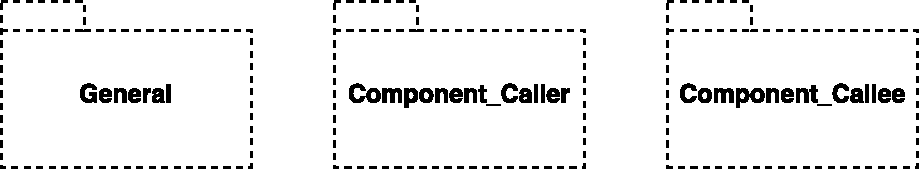
\includegraphics[width=0.5\textwidth]{NamespacesUML.pdf}
	\caption{UML class diagram representation for different namespaces in the example OBSW model}
	\label{fig: PackagesUML}
\end{figure}

\subsubsection{\textbf{Data types and events}}
A data type from the OBSW model is translated into a simple \texttt{typedef} statement from C++.

\textbf{For our example OBSW model}:
\begin{itemize}
\item The data type \texttt{IntegerType}, is translated to \texttt{typedef\allowbreak \ int8\_t IntegerType}
\item The data type \texttt{StringType}, is translated to \texttt{typedef\allowbreak \ std::string StringType} 
\end{itemize}

A subset of all possible data types from the OSRA Component Model can be translated to simple \texttt{typedef} statements as shown above. More information about the subset of data types for which this successfully works is given in the next chapter. 

The exception types from the OBSW models are translated into simple enumeration literals from C++. These exceptions, which can be thrown by a particular operation are grouped under an enumeration. This enumeration is further instantiated in a C++ struct.

\textbf{For our example OBSW model}: The three exceptions \texttt{Operand\allowbreak Exception}, \texttt{Memory\allowbreak Exception} and \texttt{Overflow\allowbreak Exception} are translated to enumeration literals. These exceptions can be thrown by \texttt{OperationAdd}, which is defined in \texttt{InterfaceB}. Hence the enumeration literals, corresponding to the exceptions, are stored together as an enumeration named \texttt{OperationAdd\allowbreak Exception\allowbreak\_InterfaceB} as shown in the \cref{fig: ExceptionsUML}. This exception is further instantiated in a C++ struct \texttt{OperationAdd\allowbreak Report\allowbreak\_InterfaceB} as shown in the \cref{fig: ExceptionsUML} 

\begin{figure}[h]
	\centering
	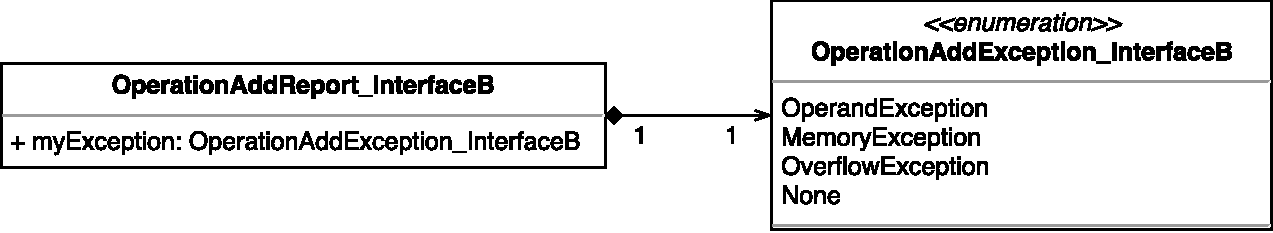
\includegraphics[width=1.0\textwidth]{ExceptionsUML.pdf}
	\caption{UML class diagram representation for exceptions in the example OBSW model}
	\label{fig: ExceptionsUML}
\end{figure}

An event from the OBSW model is mapped to an abstract base class and a corresponding concrete implementation class. As already explained, the abstract base classes hwelp in improving the testability of the generated software. Appropriate setters and getters for the event parameters are declared as pure virtual methods in the abstract base class for the event and they are implemented in their corresponding concrete implementation.

\textbf{For our example OBSW model}: The \texttt{FailureEvent} is mapped as an abstract base class named \texttt{FailureEvent\allowbreak Interface} and concrete implementation class named \texttt{FailureEvent}. Appropriate setters and getters for the event parameters \texttt{Param} and \texttt{Failure\allowbreak Event\allowbreak	Description} are declared as pure virtual methods in the \texttt{FailureEvent\allowbreak Interface} abstract base class and implemented in the \texttt{FailureEvent} concrete implementation class. An UML class diagram representation of the generated classes are as shown in \cref{fig: EventUML}.

\begin{figure}[h]
	\centering
	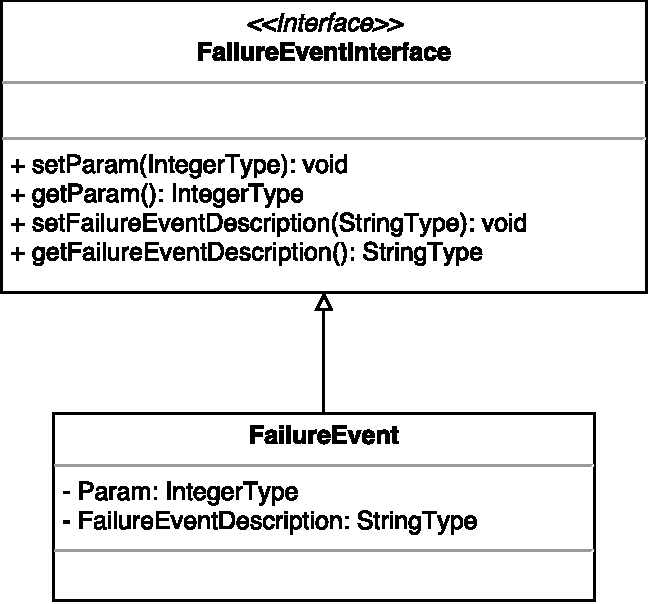
\includegraphics[width=0.6\textwidth]{EventUML.pdf}
	\caption{UML class diagram representation for event in the example OBSW model}
	\label{fig: EventUML}
\end{figure}    

All the infrastructure code entities mentioned above are present in the namespace \texttt{General}.  

\subsubsection{\textbf{Interfaces}}
An interface can be mapped to a C++ abstract base class, as in \cite{EvoRAVCodeAr}. Constituents of this abstract base class are:

\begin{itemize}
\item For each interface operation, a pure virtual method is declared in the interface class. The names and data types of the input parameters for this pure virtual method corresponds to the names and data types of the interface operation parameters. The operation parameters, with \texttt{ParameterDirectionKind} as \texttt{in} are translated to constant references and the operation parameters with \texttt{ParameterDirectionKind} as \texttt{out} or \texttt{inout} are translated to plain references. 
\item For each interface attribute parameter of type \texttt{CFG}:
\begin{itemize}
\item A class variable of name and data type corresponding to the name and data type of interface attribute is added
\item Pure virtual setter and getter methods for the interface attribute are declared. The data types and names of the input parameters in the setter and getter methods mimic the name and data type of the interface attribute.
\end{itemize} 
\item For each interface attribute parameter of type \texttt{MIS}, which is fixed and is not variable \cite{SpecMetamodel}: 
\begin{itemize}
\item A \texttt{const} class variable of name and data type corresponding to the name and data type of interface attribute is added
\item No getter and setter methods are added
\end{itemize}
\item For each interface attribute of type \texttt{DAT}, which are modifiable by the component only and not by external entities \cite{SpecMetamodel}:
\begin{itemize}
\item A class variable of name and data type corresponding to the name and data type of interface attribute is added
\item No getter and setter methods are added  
\end{itemize}   
\end{itemize}

\textbf{For our example OBSW model} The C++ classes shown in \cref{fig: InterfacesUML} are generated:
\begin{itemize}
\item \texttt{InterfaceA} along with the operation \texttt{CallOperationAdd} is mapped to an abstract base class \texttt{InterfaceA} with a pure virtual method \texttt{CallOperationAdd}. 
\item \texttt{InterfaceB} has one operation \texttt{OperationAdd} and one interface attribute parameter \texttt{StatusValue} of type \texttt{CFG}. These are mapped to an abstract base class named \texttt{InterfaceB} with the following pure virtual methods:
\begin{itemize}
\item \texttt{OperationAdd} with two input parameters of type \texttt{const\allowbreak \ IntegerType\&} and one input parameter of type \texttt{IntegerType\&}
\item getter method for the interface attribute \texttt{StatusValue} with an input parameter of type \texttt{IntegerType\&}
\item setter method for the interface attribute \texttt{StatusValue} with an input parameter of type \texttt{const\allowbreak \ IntegerType\&}
\end{itemize} 
\end{itemize}

\begin{figure}[h]
	\centering
	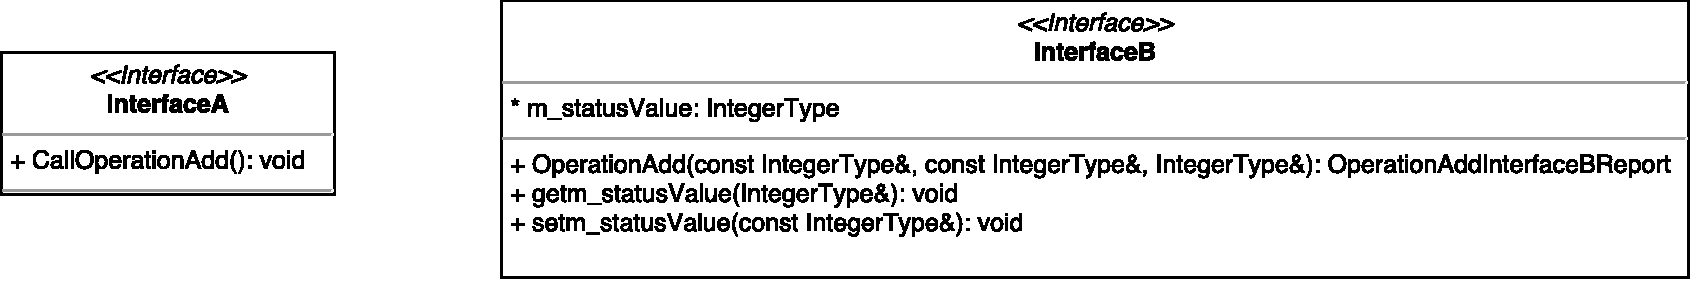
\includegraphics[width=1.0\textwidth]{InterfacesUML.pdf}
	\caption{UML class diagram representation for interfaces in the example OBSW model}
	\label{fig: InterfacesUML}
\end{figure}

Because of the corner case that multiple interfaces can have exactly same operations, it is necessary to refine these interfaces using the interface helper abstract base classes as shown in \cref{fig: Interface helpers UML}. In each interface helper class:
\begin{itemize}
\item Implementations for all the inherited pure virtual methods from the parent interface are provided
\item The implementations consist of simple method calls to new pure virtual methods
\item These new pure virtual methods have method signatures same as the pure virtual methods that are inherited and implemented. However, it is important to note that the names of these new pure virtual methods are different from the inherited pure virtual methods, as shown in the \cref{Listing: Interface helper Impl} 
\end{itemize}

\begin{figure}[h]
	\centering
	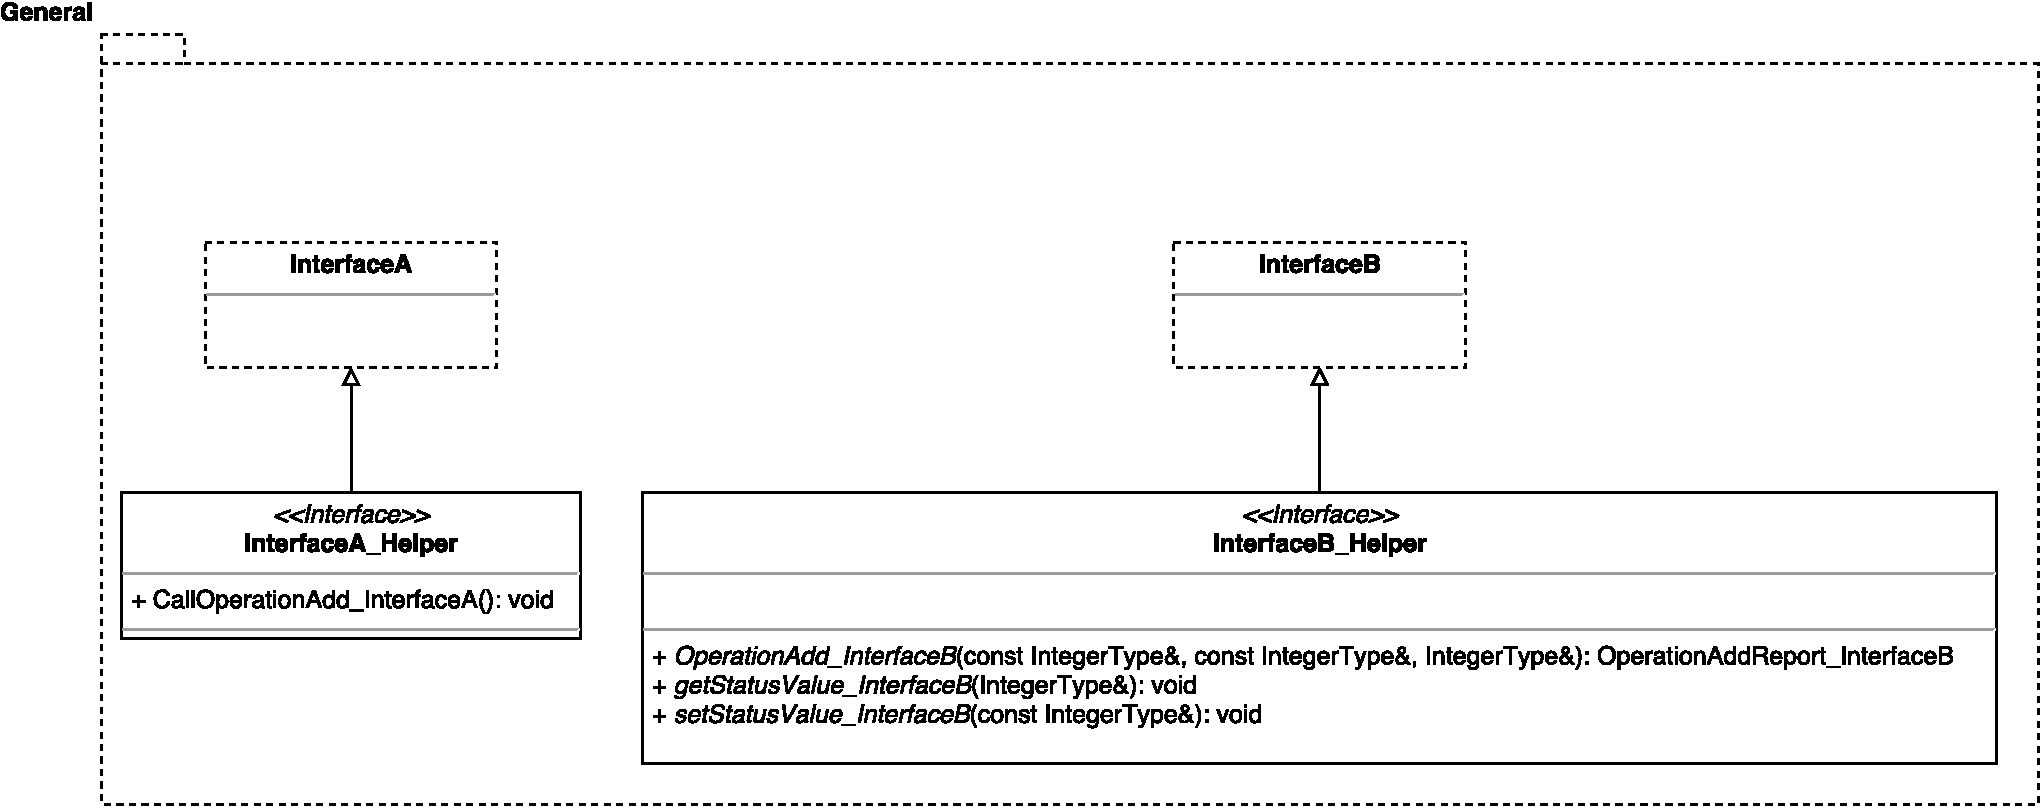
\includegraphics[width=0.8\textwidth]{InterfaceHelpersUML.pdf}
	\caption{UML class diagram representation for interface helpers in the example OBSW model}
	\label{fig: Interface helpers UML}
\end{figure}

\begin{Listing}
\begin{lstlisting}[language=C++]
class InterfaceA {
public:
	InterfaceA(){}
	virtual ~InterfaceA(){}
	virtual void callOperationAdd(void) = 0;
};

class InterfaceA_Helper: public InterfaceA {
public:
	InterfaceA_Helper(){}
	virtual ~InterfaceA_Helper(){}
	virtual void callOperationAdd_InterfaceA(void) = 0; //New pure virtual method
	virtual void callOperationAdd(void)final {return (callOperationAdd_InterfaceA());}
};
\end{lstlisting}
\caption{Code excerpt from the generated code for \texttt{InterfaceA\allowbreak\_Helper}}
\label{Listing: Interface helper Impl}
\end{Listing}

\textbf{For our example OBSW model}:
\begin{itemize}
\item \texttt{InterfaceA\allowbreak\_Helper} is defined, which inherits from the interface \texttt{InterfaceA} and which implements the pure virtual method in the parent interface \texttt{InterfaceA}. The implementation contains a simple call to a new pure virtual method added to the original method name from the parent interface as shown in the \cref{Listing: Interface helper Impl}.

\item \texttt{InterfaceB\allowbreak\_Helper} is defined, which inherits from the interface \texttt{InterfaceB} and which implements all the pure virtual methods in the parent interface \texttt{InterfaceB}. Each implementation contain a simple call to the new pure virtual methods added. The \texttt{InterfaceB\allowbreak\_Helper} class is designed and implemented the same way as \texttt{InterfaceA\allowbreak\_Helper} is designed in the code excerpt in \cref{Listing: Interface helper Impl}   
\end{itemize}

The combined effect is that now, more than one original parent interfaces (resembling model entities) can have same operations and interface attributes. The refined interfaces redefine the methods from the original parent interfaces, so that there are no confusions between operations from different interfaces. Of course, a straight forward solution would have been to incorporate the concept of namespaces from C++, but it is not suitable for this design and the reason is explained later in this section. 

For each interface operation and interface attribute in an interface, a C++ struct is defined to carry around the values of the operation parameters or the values of the interface attributes. These data structures come in handy, when the interface operations or interface attribute access operations need to be accessed asynchronously. The data structures also hold general purpose polymorphic function wrappers from C++11 standard to store the call-back functions wherever appropriate. 

\textbf{For our example OBSW model}:
\begin{itemize}
\item A struct \texttt{OperationAdd\allowbreak Struct\_\allowbreak InterfaceB} is defined as shown in \cref{fig: Operation structs UML}
\item A struct \texttt{StatusValue\allowbreak Struct\_\allowbreak InterfaceB} is defined as shown in \cref{fig: Operation structs UML}
\end{itemize} 

\begin{figure}[h]
	\centering
	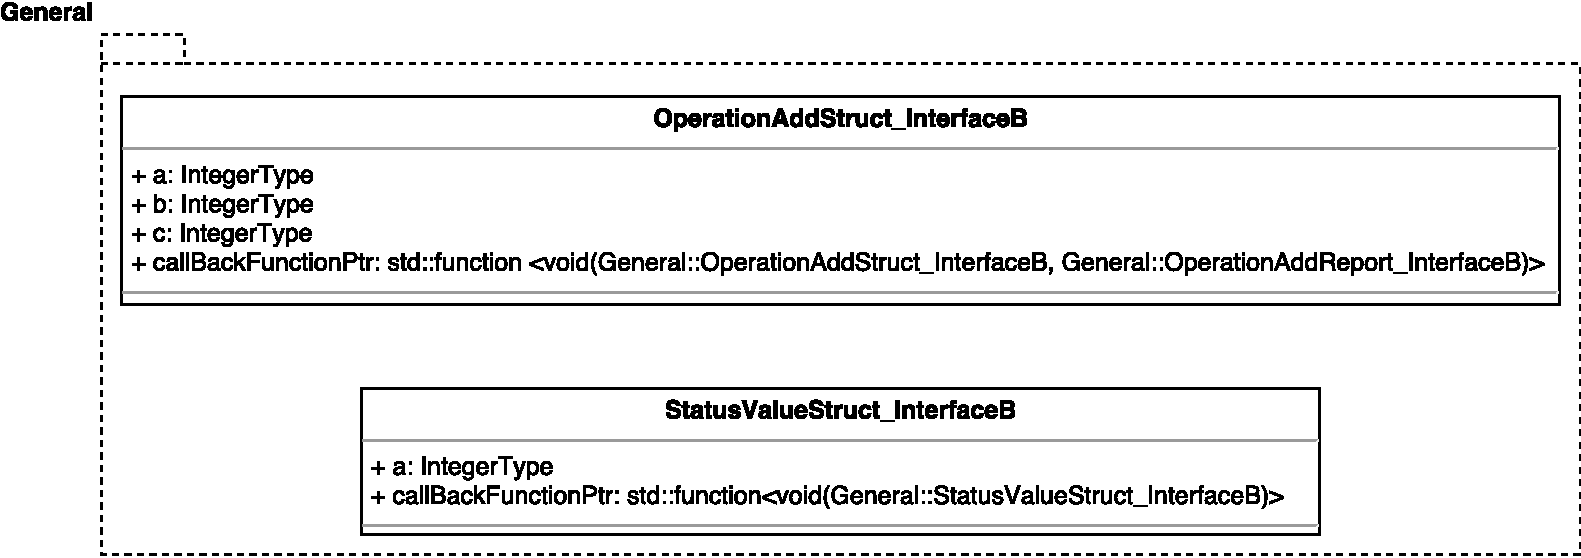
\includegraphics[width=0.8\textwidth]{OperationStructsUML.pdf}
	\caption{UML class diagram representation of data structures for interface operation and interface attribute in the example OBSW model}
	\label{fig: Operation structs UML}
\end{figure} 

All the infrastructure code entities mentioned above are present in the namespace \texttt{General}.

\subsubsection{\textbf{Parameter channels and parameter queues}}
The data structures which are defined to carry around the values of the operation parameters or values of the interface attributes, need to be pushed onto parameter channels, each one of which is supported in the back end by corresponding parameter queue.

\textbf{For our example OBSW model}: \texttt{Parameter\allowbreak Channel} and \texttt{Parameter\allowbreak Queue} C++ classes as shown in \cref{fig: Parameter channel UML} are defined. These classes can be reused for any OBSW model. 

\begin{figure}[h]
	\centering
	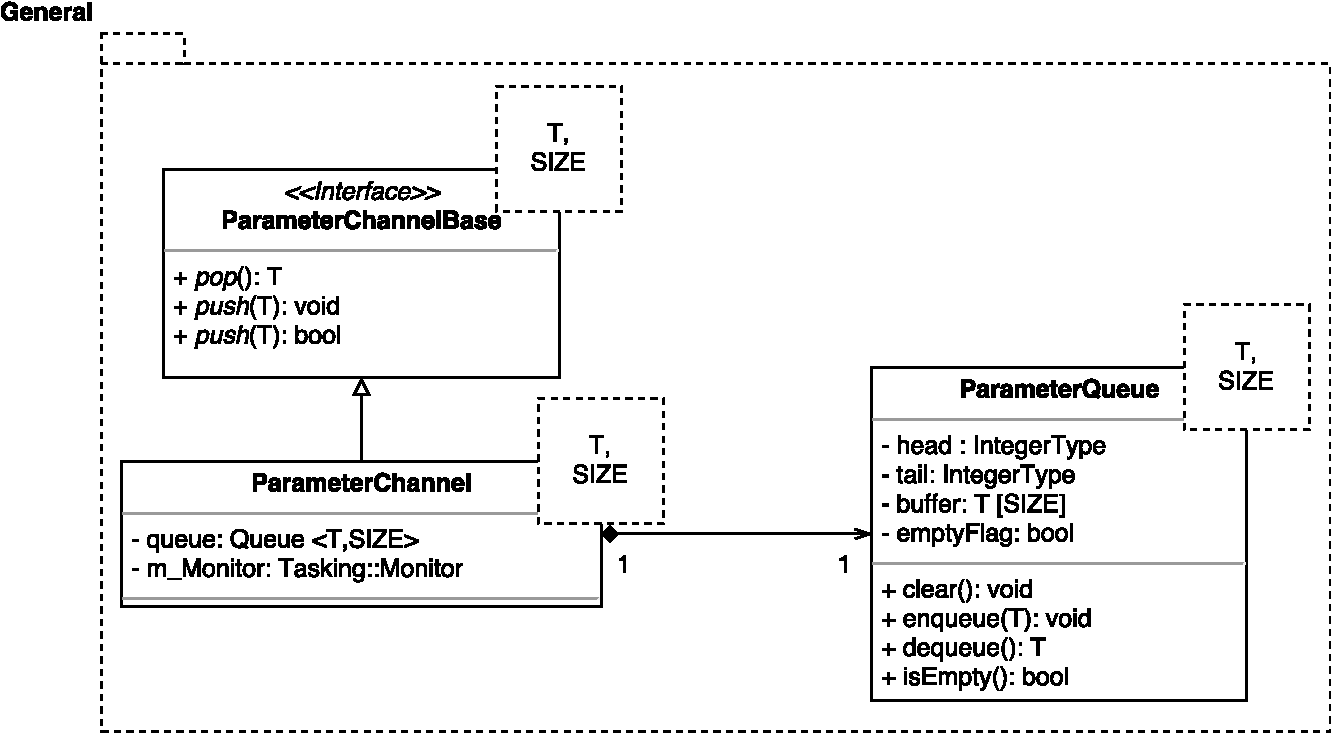
\includegraphics[width=1.0\textwidth]{ParameterChannelQueue.pdf}
	\caption{UML class diagram representation of parameter channel and parameter queue in the example OBSW model}
	\label{fig: Parameter channel UML}
\end{figure}

All the infrastructure code entities mentioned above are present in the namespace \texttt{General}.   

\subsubsection{\textbf{Event emitter ports and event receiver ports}}
The event emitter port for a particular event is mapped as an abstract base class and a corresponding concrete implementation class in C++. The event receiver port for a particular event is mapped only as an abstract base class. The abstract base class for event receiver port also contains pure virtual methods in order to safely interleave the reception of events.  

\textbf{For our example OBSW model}: The \texttt{FailureEvent\allowbreak EmitterPort} is mapped as a pair of abstract base class and a concrete implementation class as shown in \cref{fig: Event emitter port UML}.  

\textbf{For our example OBSW model}: The \texttt{FailureEvent\allowbreak ReceiverPort} is mapped to an abstract base class as shown in \cref{fig: Event receiver port UML}.

\begin{figure}[h]
	\centering
	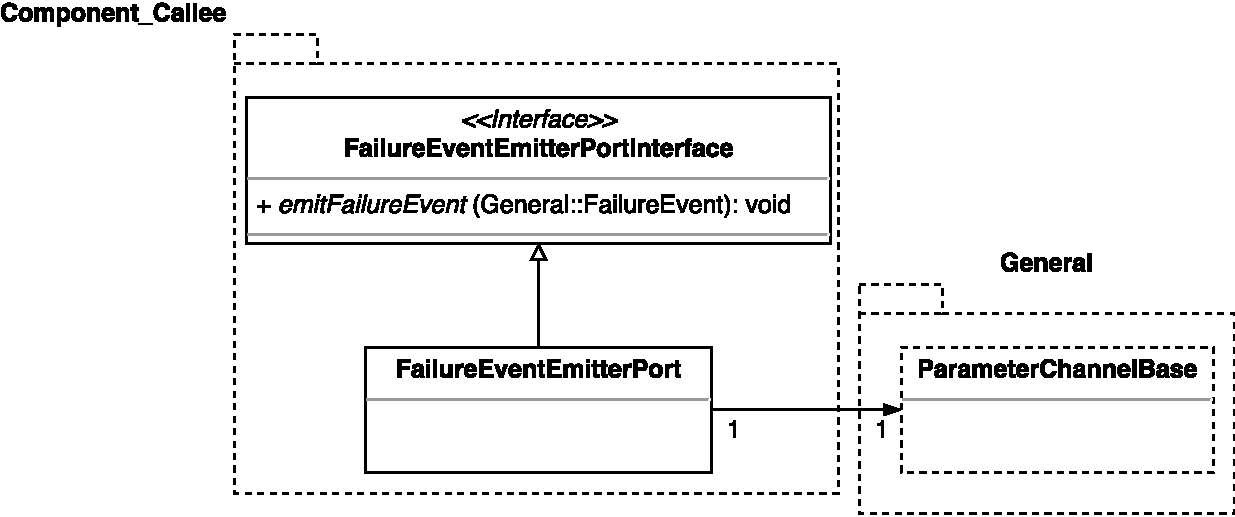
\includegraphics[width=1.0\textwidth]{EventEmitterPortUML.pdf}
	\caption{UML class diagram representation of event emitter port in the example OBSW model}
	\label{fig: Event emitter port UML}
\end{figure}

\begin{figure}[h]
	\centering
	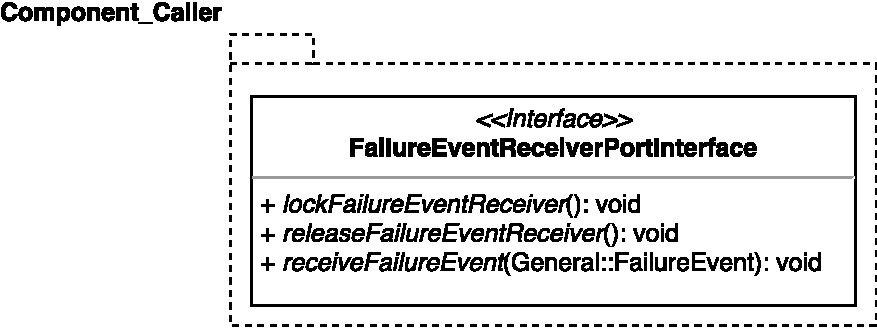
\includegraphics[width=0.8\textwidth]{EventReceiverPortUML.pdf}
	\caption{UML class diagram representation of event receiver port in the example OBSW model}
	\label{fig: Event receiver port UML}
\end{figure} 

The \texttt{FailureEvent\allowbreak Emitter\allowbreak Port\allowbreak Interface} and \texttt{FailureEvent\allowbreak Emitter\allowbreak Port} classes are defined in the namespace \texttt{Component\allowbreak \_Callee}. 

The \texttt{FailureEvent\allowbreak Receiver\allowbreak Port\allowbreak Interface} is defined in the namespace \texttt{Component\allowbreak\_Caller}.

\subsubsection{\textbf{Component types}}
A component type can be mapped to an abstract base class in C++. A component type must provide all the operations that are listed in the provided interfaces of the component \cite{CompBasedProcess}. Hence it inherits from all the interface helper classes which are referenced by its provided interfaces as in \cite{EvoRAVCodeAr} 

This is where interface helper classes, with redefined operations come in handy, because C++ does not distinguish between operations with same signatures, although they are inherited from different namespaces. A component type must also inherit from the mapped abstract base classes for event receiver ports.

A component type must also have pure virtual methods which obtain and release the semaphores for the concurrent access of different operations that it provides. In addition to these, pure virtual methods need to be added, which act as call-back functions for the operations, that the component type's required interface ports request to be released asynchronously.   

\textbf{For our example OBSW model}:
\begin{itemize}
\item As shown in \cref{fig: Component type Caller UML} \texttt{ComponentType} in the namespace \texttt{Component\_Caller} inherits from the \texttt{InterfaceA\allowbreak\_Helper} and also inherits from the abstract base class \texttt{FailureEvent\allowbreak ReceiverPort\allowbreak Interface}. 
It has pure virtual methods meant for:

\begin{itemize}
\item Obtaining and releasing of semaphores for concurrent accesses of the operation \texttt{CallOperationAdd\allowbreak\_InterfaceA}
\item Call-back function for the operation \texttt{OperationAdd}
\item Call-back function for the getter operation of the interface attribute \texttt{StatusValue} 
\end{itemize}

\item A shown in \cref{fig: Component type Callee UML} \texttt{ComponentType} in the namespace \texttt{Component\_Callee} inherits from the \texttt{InterfaceB\allowbreak\_Helper}. 
It has pure virtual methods meant for:

\begin{itemize}
\item Obtaining and releasing of semaphores for concurrent access of the operation {OperationAdd\allowbreak\_InterfaceB}
\item Obtaining and releasing of semaphores for concurrent access of the setter and getter operations for the interface attribute \texttt{StatusValue}
\end{itemize}   
\end{itemize}

\begin{figure}[h]
	\centering
	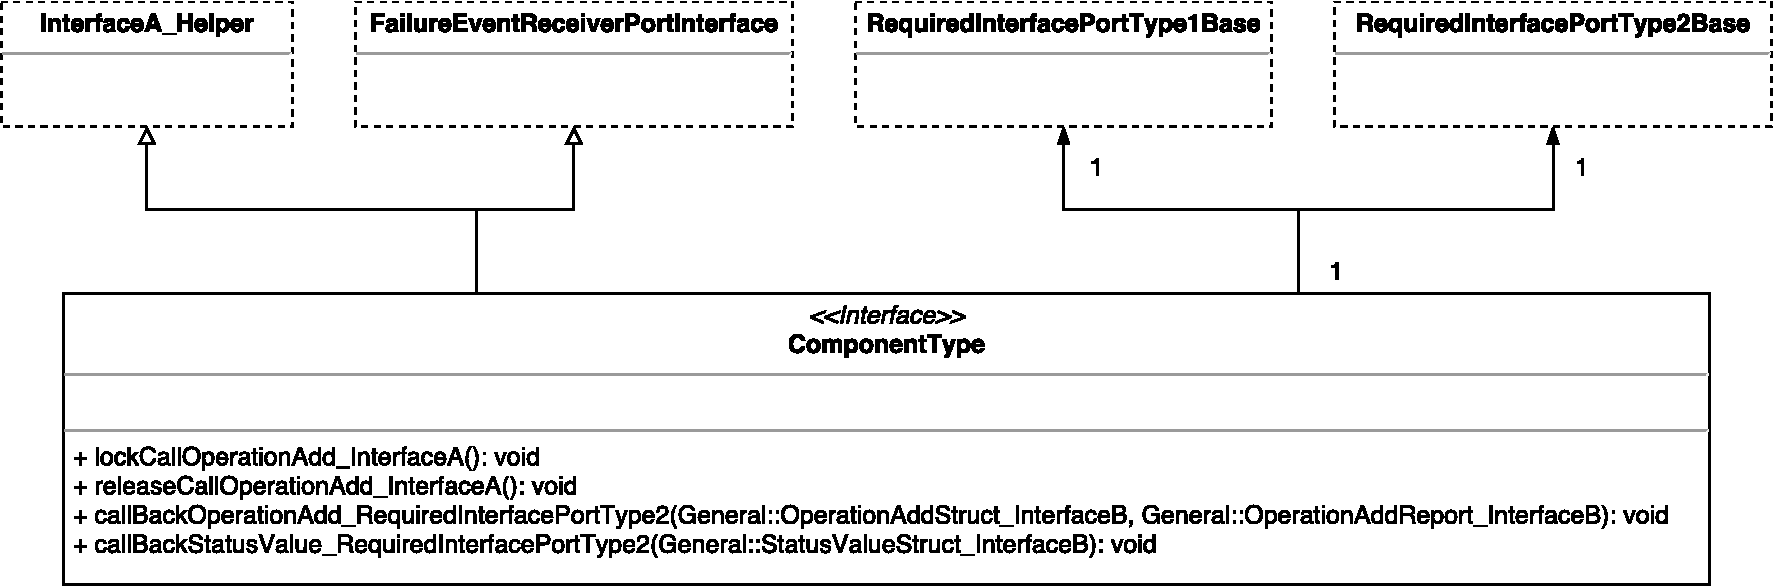
\includegraphics[width=1.0\textwidth]{ComponentTypeCallerUML.pdf}
	\caption{UML class diagram representation of component type for \texttt{Component\allowbreak\_Caller} in the example OBSW model}
	\label{fig: Component type Caller UML}
\end{figure} 

\begin{figure}[h]
	\centering
	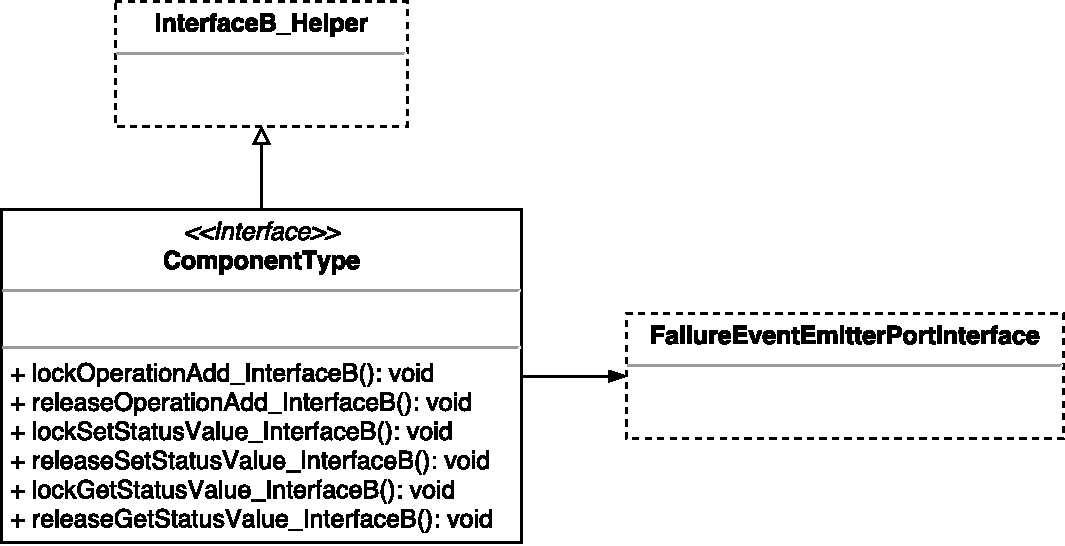
\includegraphics[width=0.8\textwidth]{ComponentTypeCalleeUML.pdf}
	\caption{UML class diagram representation of component type for \texttt{Component\allowbreak\_Callee} in the example OBSW model}
	\label{fig: Component type Callee UML}
\end{figure} 

\subsubsection{\textbf{Required interface ports}}
A required interface port is mapped as an abstract base class and a corresponding concrete implementation class in C++. The required interface subsumed by a particular component type has various operations that it might request and each operation has information specified whether the required interaction kind is \texttt{synchronous} or \texttt{asynchronous} \cite{SpecMetamodel,CompBasedProcess}. 

Each required interface port refers to one interface type and for each operation in the required interface port, a pure virtual method is added to the abstract base class. The signatures of these methods depend on whether the operations would be requested with an asynchronous release pattern or synchronous release pattern.

In case of interface operations:
\begin{itemize}
\item If the desired interaction kind for the operation is \texttt{synchronous}, then the signature of the method in the abstract base class is same as the corresponding method in the abstract base class for the interface, as shown in \cref{fig: Required interface port1 UML}.
\item If the desired interaction kind for the operation is \texttt{asynchronous}, then the signature of the method in the abstract base class bears no resemblance to the corresponding method in the abstract base class for the interface. It is changed as shown in \cref{fig: Required interface port2 UML} to replace the \texttt{out} and \texttt{inout} parameters with a single pointer to the desired call-back function 
\end{itemize}

In case of interface attributes:
\begin{itemize}
\item For the setter operation, signature of the method in the abstract class is same as the corresponding method in the abstract base class for the interface, as shown in \cref{fig: Required interface port1 UML} and \cref{fig: Required interface port2 UML}
\item If the desired interaction kind for the getter operation is \texttt{synchronous}, then the signature of the method in the abstract class is same as the corresponding method in the abstract base class for the interface, as shown in \cref{fig: Required interface port1 UML}. 
\item If the desired interaction kind for the getter operation is \texttt{asynchronous}, then the signature of the method in the abstract base class bears no resemblance to the corresponding method in the abstract base class for the interface. It is changed as shown in \cref{fig: Required interface port2 UML} to replace the method parameter with a single pointer to the desired call-back function  
\end{itemize} 

The concrete implementation of any method, for example, as the one shown in the code excerpt in \cref{Listing: Required interface port1 Impl} is fairly simple, if the desired interaction kind for the corresponding operation is \texttt{synchronous}. The implementation consists of a simple method call to the corresponding operation in the abstract base class of the bound provided interface port.

\begin{Listing}
\begin{lstlisting}[language=C++]
General::OperationAddReport_InterfaceB RequiredInterfacePortType1::OperationAdd (const IntegerType& a,const IntegerType& b,IntegerType& c) {
	General::OperationAddReport_InterfaceB myReport;
	myReport = m_targetProvidedInterfacePort.OperationAdd(a,b,c); //Simple method call
	return myReport;
}
\end{lstlisting}
\caption{Code excerpt from the generated code for requesting service \texttt{OperationAdd} in \texttt{Required\allowbreak InterfacePort\allowbreak Type1}}
\label{Listing: Required interface port1 Impl}
\end{Listing}

The concrete implementation for any method, for example, the one as shown in code excerpt in \cref{Listing: Required interface port2 Impl} is fairly complex, if the desired interaction kind for the corresponding operation is \texttt{asynchronous}. It would do the following things: 
\begin{itemize}
\item Make local copies of all the method parameters (if any)
\item Pack them in the instances of data structures designed to carry the corresponding parameters
\item Simple method call to the corresponding operation in the abstract base class of the bound provided interface port
\end{itemize}

\begin{Listing}
\begin{lstlisting}[language=C++]
void RequiredInterfacePortType2::getStatusValue(callBackStatusValue_RequiredInterfacePortType2 callBackFunctionPtr) {
	StatusValueStruct_InterfaceB myStruct; 
	myStruct.callBackFunctionPtr = std::bind(callBackFunctionPtr,m_myCallerInstance,std::placeholder::_1);
	m_targetProvidedInterfaceSlot.getStatusValue_Receiver(myStruct); //Simple method call
}
\end{lstlisting}
\caption{Code excerpt from the generated code for interface attribute \texttt{StatusValue} access in \texttt{Required\allowbreak InterfacePort\allowbreak Type2}}
\label{Listing: Required interface port2 Impl}
\end{Listing}

It is clear that local copies of the method parameters need to be made because the desired interaction kind is \texttt{asynchronous}.             

\textbf{For our example OBSW model}: The following C++ classes are defined:
\begin{itemize}
\item \texttt{RequiredInterface\allowbreak PortType1Base} abstract base class and its corresponding \texttt{Required\allowbreak InterfacePort\allowbreak Type1} concrete implementation class.
\item \texttt{RequiredInterface\allowbreak PortType2Base} abstract base class and its corresponding \texttt{Required\allowbreak InterfacePort\allowbreak Type2} concrete implementation class
\end{itemize}

The \texttt{RequiredInterface\allowbreak PortType1Base} and \texttt{RequiredInterface\allowbreak PortType2Base} have pure virtual methods as per the general description and they have to be implemented in the concrete implementation classes \texttt{Required\allowbreak InterfacePort\allowbreak Type1} and \texttt{Required\allowbreak InterfacePort\allowbreak Type2} respectively. The concrete implementations are in line with the description as in the general case above.

\begin{figure}[h]
	\centering
	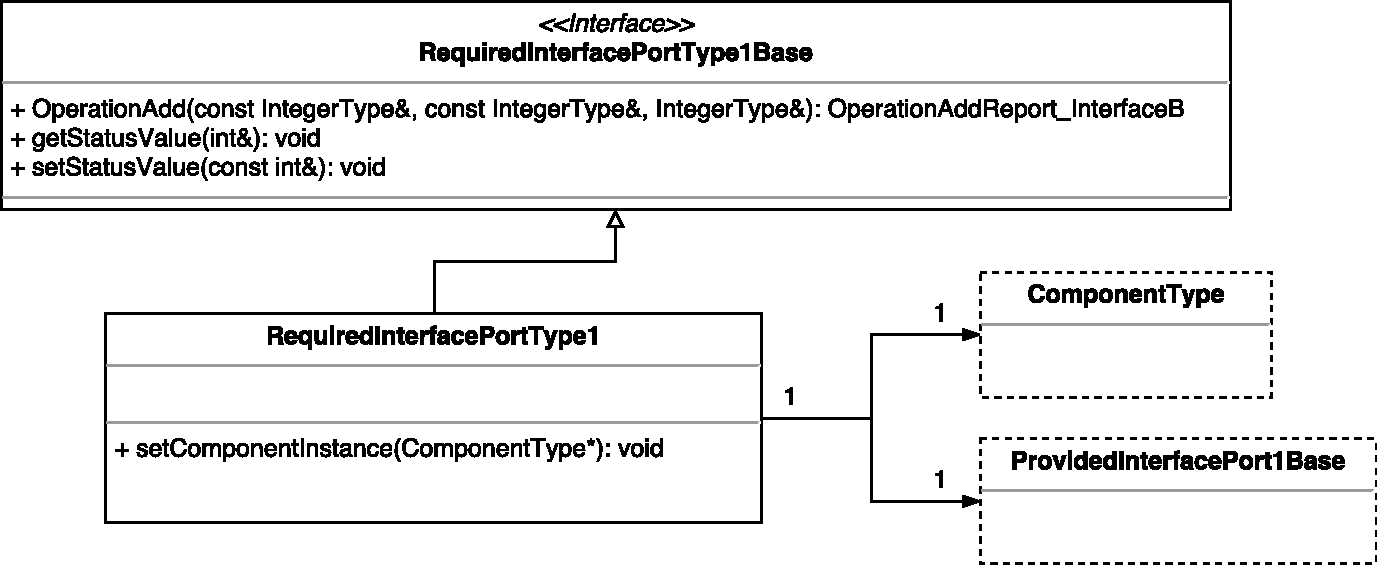
\includegraphics[width=1.0\textwidth]{RequiredInterfacePort1UML.pdf}
	\caption{UML class diagram representation of \texttt{Required\allowbreak InterfacePort\allowbreak Type1} for \texttt{Component\allowbreak\_Caller} in the example OBSW model}
	\label{fig: Required interface port1 UML}
\end{figure}

\begin{figure}[h]
	\centering
	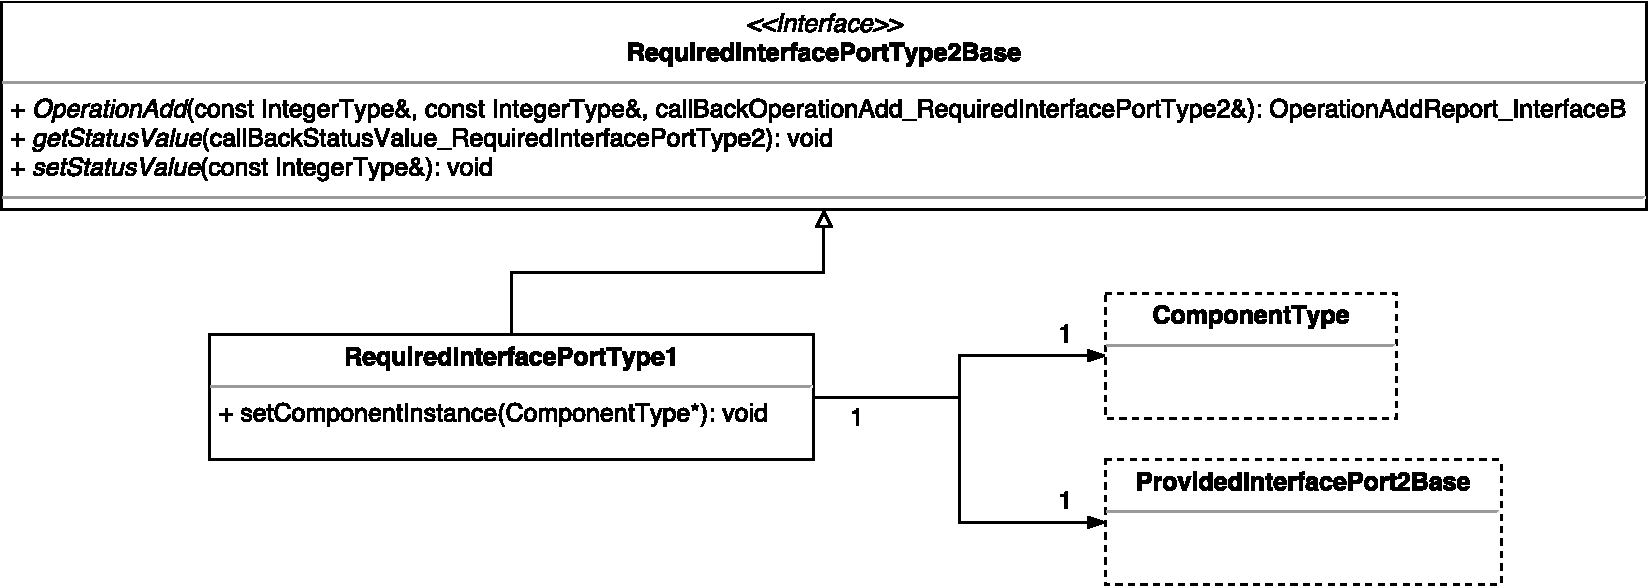
\includegraphics[width=1.0\textwidth]{RequiredInterfacePort2UML.pdf}
	\caption{UML class diagram representation of \texttt{Required\allowbreak InterfacePort\allowbreak Type2} for \texttt{Component\allowbreak\_Caller} in the example OBSW model}
	\label{fig: Required interface port2 UML}
\end{figure}

All the C++ classes mentioned above are present in the namespace \texttt{Component\allowbreak\_Caller}. As the component type \texttt{Component\allowbreak\_Callee} does not have any required interface ports, no C++ classes related to required interface ports are defined in the namespace \texttt{Component\allowbreak\_Callee}. 

\subsubsection{\textbf{Component implementations}}
A component implementation can be mapped in C++ as a concrete implementation of its abstract component type base class. as in \cite{EvoRAVCodeAr}. It implements all the pure virtual methods that are inherited from its component type. It also has actual instances of semaphores for allowing safe concurrent accesses to the implemented methods and for safe interleaving between concurrent receptions of events of the same type.

In case of components that promote multiple provided interface ports which refer to the same interface type, it is necessary to provide multiple implementations for the operations in the provided interfaces. In order to solve this problem a class hierarchy as shown in \cref{fig: Component implementation Callee UML} is decided upon in this Master thesis:

\begin{itemize}
\item A component implementation abstract base class is designed which contains implementations for inherited pure virtual methods related to acquiring and releasing of semaphores. Also the the inherited pure virtual methods which are provided only once are implemented here
\item The Component implementation abstract base class is further extended by dummy abstract base classes. A dummy base class is added for each of the provided interface ports which refer to the same interface type. These dummy abstract base classes help in testing of the implementations of the services which are provided by multiple provided interfaces. With the help of these dummy abstract base classes, mock implementation classes can be easily created and used in testing \cite{InvOfCntrlurl}  
\item These dummy abstract base classes are extended by concrete implementation classes which provide different concrete implementations for all the inherited operations except the ones, which are already implemented in the component implementation abstract base class
\item As it is a necessity to have only one instantiable concrete implementation per component \cite{EvoRAVCodeAr,SpecMetamodel,CompBasedProcess}, all the concrete implementations are inherited one last time in a component implementation class. This instance is now deployable on the hardware platform
\end{itemize}
 
\textbf{For our example OBSW model}:
\begin{itemize}
\item \texttt{Component\allowbreak Implementation} concrete implementation class in the namespace \texttt{Component\_Caller} inherits from the abstract base class \texttt{Component\_Type} in namespace \texttt{Component\allowbreak\_Caller} as shown in \cref{fig: Component implementation Caller UML}. It provides implementation for all the inherited pure virtual methods
\item Because the \texttt{ComponentType} in the namespace \texttt{Component\_Callee} has two provided interface ports namely, \texttt{Provided\allowbreak Interface\allowbreak Port1} and \texttt{Provided\allowbreak Interface\allowbreak Port2}, which refer to \texttt{InterfaceB}, the following classes as shown in \cref{fig: Component implementation Callee UML} are created in the namespace \texttt{Component\_Callee}:
\begin{itemize}
\item \texttt{ComponentImplementation\allowbreak Base} which is an abstract base class, but provides implementation for inherited pure virtual methods related to acquiring and releasing of semaphores
\item \texttt{Component\allowbreak Implementation\allowbreak Provided\allowbreak Interface1\allowbreak Base} and \texttt{Component\allowbreak Implemen\allowbreak tation\allowbreak Provided\allowbreak Interface2\allowbreak Base} which are two dummy abstract base classes
\item \texttt{Component\allowbreak Implementation\allowbreak Provided\allowbreak Interface1} and \texttt{Component\allowbreak Impl\allowbreak emen\allowbreak tation\allowbreak Provided\allowbreak Interface2} which provide different implementations for all the inherited operations except the ones implemented in \texttt{Component\allowbreak Implementation\allowbreak Base}
\item \texttt{Component\allowbreak Implementation} which inherits from both \texttt{Component\allowbreak Implemen\allowbreak tation\allowbreak Provided\allowbreak Interface1} and \texttt{Component\allowbreak Implementation\allowbreak Provided\allowbreak Inter\allowbreak face2}
\end{itemize}   
\end{itemize}

\begin{figure}[h]
	\centering
	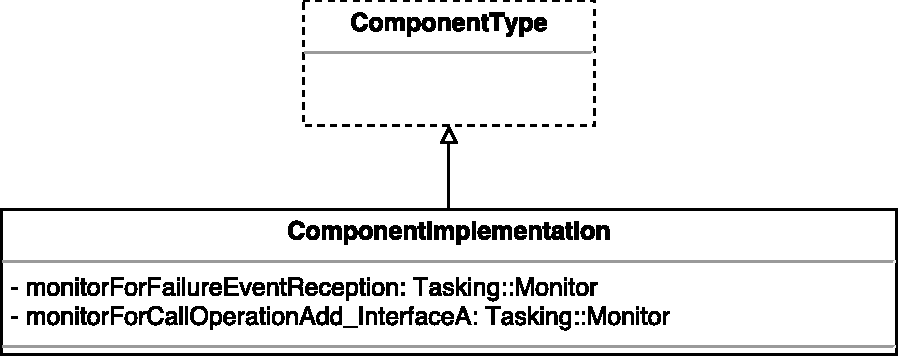
\includegraphics[width=0.8\textwidth]{ComponentImplementationCallerUML.pdf}
	\caption{Code excerpt from the generated code for interface attribute \texttt{StatusValue} access in \texttt{Required\allowbreak InterfacePort\allowbreak Type2}}
	\label{fig: Component implementation Caller UML}
\end{figure} 

\begin{figure}[h]
	\centering
	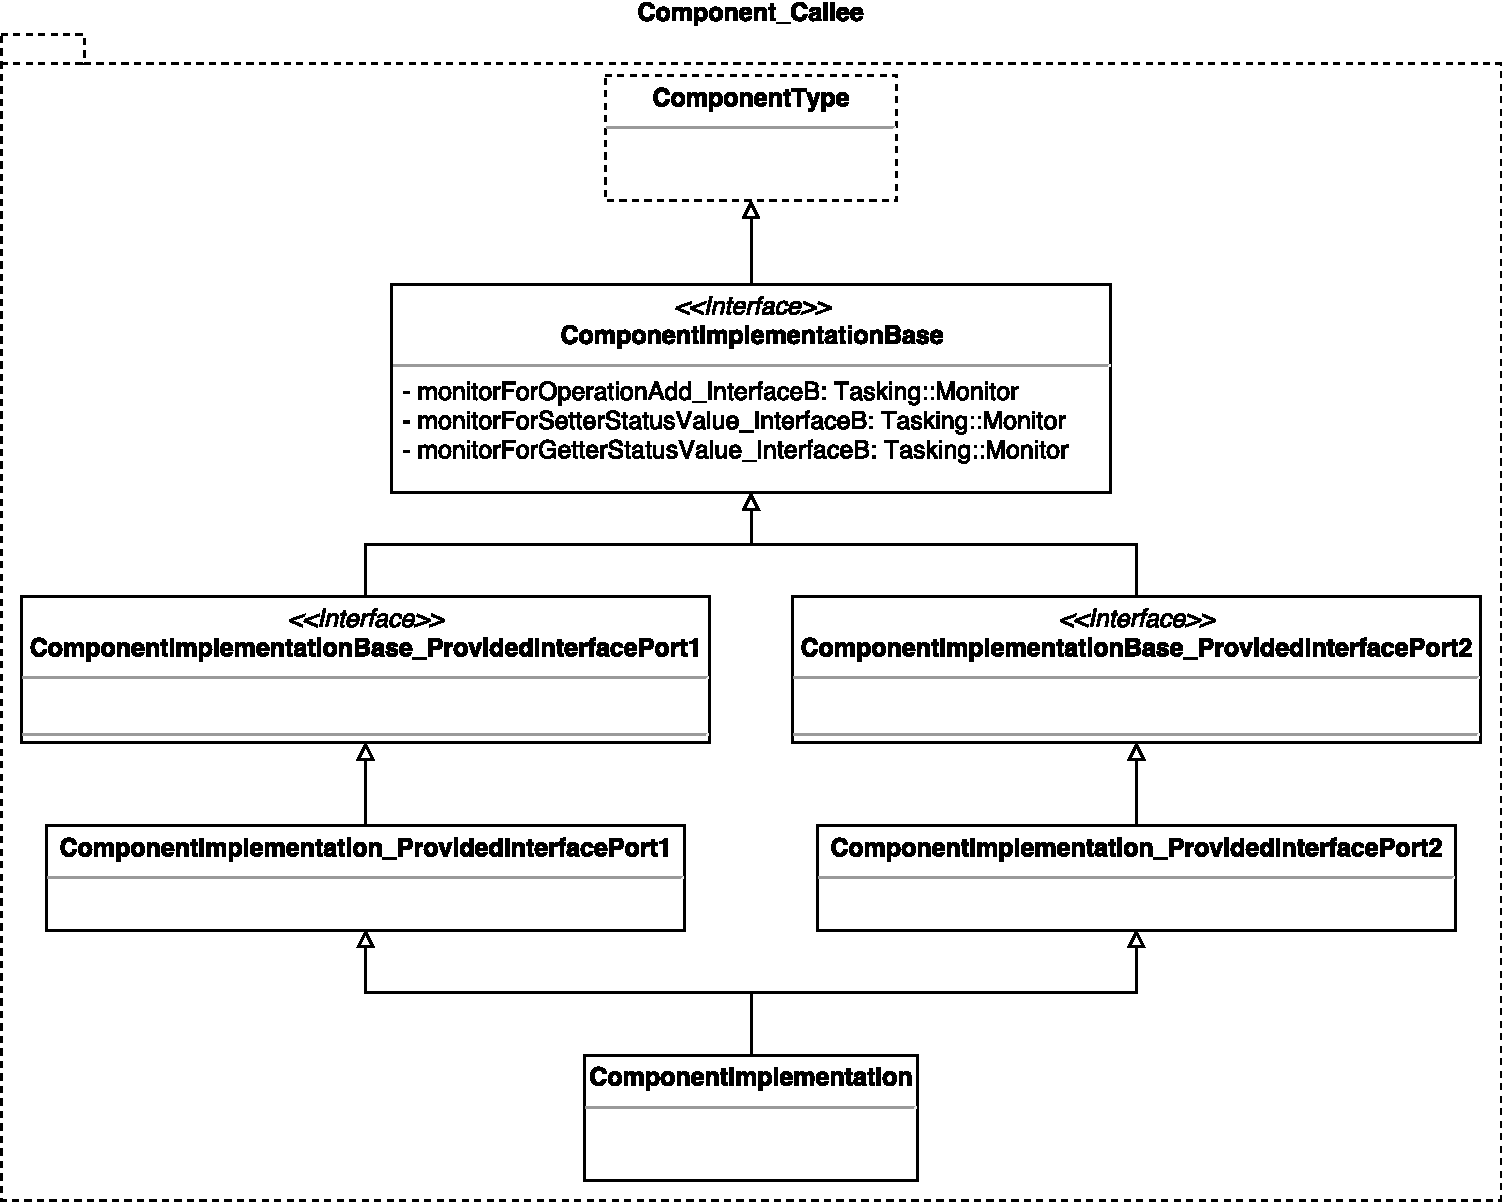
\includegraphics[width=1.0\textwidth]{ComponentImplementationCalleeUML.pdf}
	\caption{Code excerpt from the generated code for interface attribute \texttt{StatusValue} access in \texttt{Required\allowbreak InterfacePort\allowbreak Type2}}
	\label{fig: Component implementation Callee UML}
\end{figure}

\subsubsection{\textbf{Provided interface ports}}
A provided interface port is mapped to an abstract base class and a corresponding concrete implementation class as shown in \cref{fig: Provided interface port1 UML} and \cref{fig: Provided interface port2 UML}. The provided interface promoted by a particular component type has various operations that are provided and each operation has a desired release pattern attached as a non-functional/extra-functional property \cite{SpecMetamodel,CompBasedProcess}. Each provided interface port refers to one interface type and for each operation in the provided interface port, a pure virtual method is added to the abstract base class. The signatures of these methods depend on whether these operations are requested with a synchronous release pattern or an asynchronous release pattern.

In case of interface operations:
\begin{itemize}
\item If the interface operation on the provided interface is expected to be called synchronously, then the signature of the method in the abstract base class is same as the corresponding method in the abstract base class for the interface, as shown in \cref{fig: Provided interface port1 UML} for \texttt{OperationAdd}
\item If the interface operation on the provided interface is expected to be called asynchronously, then the signature of the method in the abstract base class is changed as shown in \cref{fig: Provided interface port2 UML} for \texttt{OperationAdd}, to accept a data structure designed to carry the values of the parameters for the operation along with a function-wrapper for the call-back function     
\end{itemize}   

In case of interface attributes:
\begin{itemize}
\item For the operations which set and get the values of the interface attributes synchronously, the signatures of the methods in the abstract base class are same as the corresponding method in the abstract base class for the interface
\item For the operations which set and get the values of the interface attributes asynchronously, the signatures of the methods in the abstract base class are changed to accept a data structure designed to carry the values of the interface attribute, as shown in \cref{fig: Provided interface port2 UML}. The data structure would also contain a valid function-wrapper for the call-back function in case of getter operation for the interface attribute.  
\end{itemize}

The following additional pure virtual methods are added to the abstract class for a provided interface port:
\begin{itemize}
\item For each interface operation and interface attribute setter/getter operation which is called asynchronously, an additional pure virtual method is added to store the address of the task channel, to which the data structure corresponding to the operation needs to be pushed
\item For storing the reference to their corresponding component implementation base class as shown in \cref{fig: Provided interface port1 UML} and \cref{fig: Provided interface port2 UML}
\item As shown in \cref{fig: Provided interface port UML}, for storing the reference of the task from tasking framework which is responsible for periodically requesting the service in the provided interface port which has the interaction kind set to \texttt{cyclic}. 
\end{itemize}

\begin{figure}[h]
	\centering
	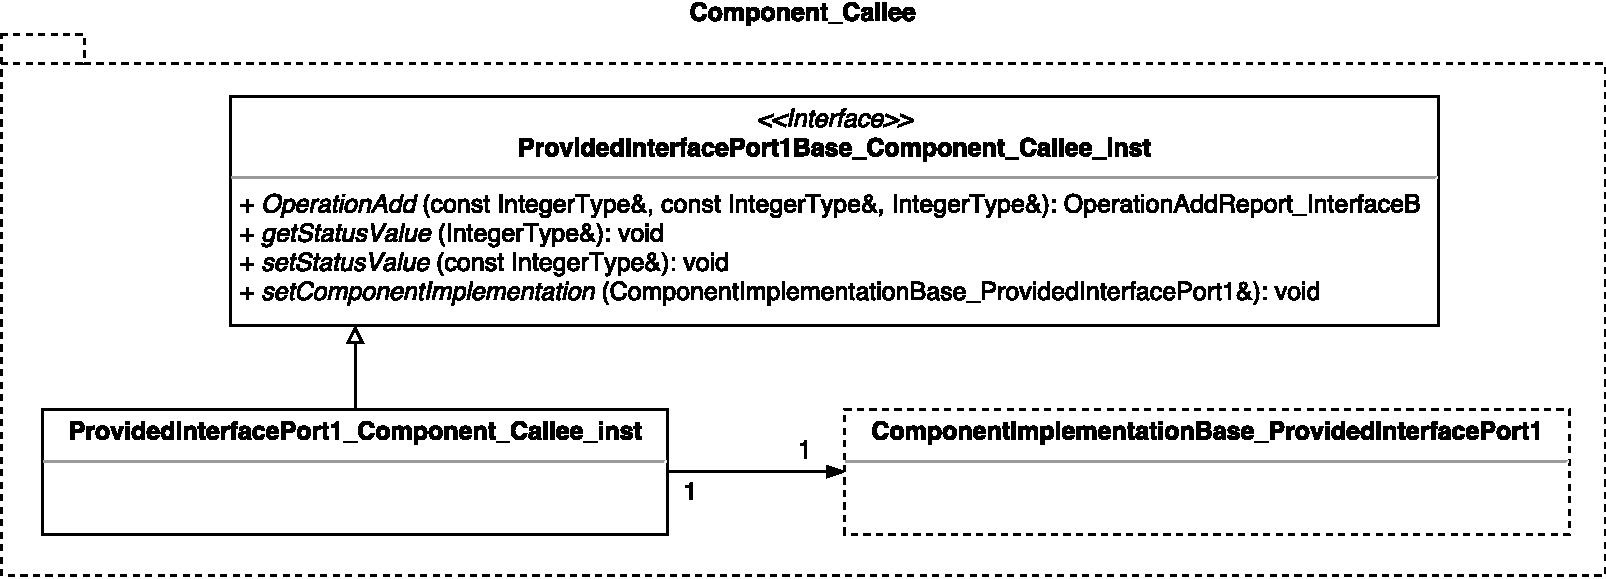
\includegraphics[width=1.0\textwidth]{ProvidedInterfacePort1UML.pdf}
	\caption{UML class diagram representation of \texttt{Provided\allowbreak Interface\allowbreak Port1} for \texttt{Component\allowbreak\_Callee} in the example OBSW model}
	\label{fig: Provided interface port1 UML}
\end{figure}

\begin{figure}[h]
	\centering
	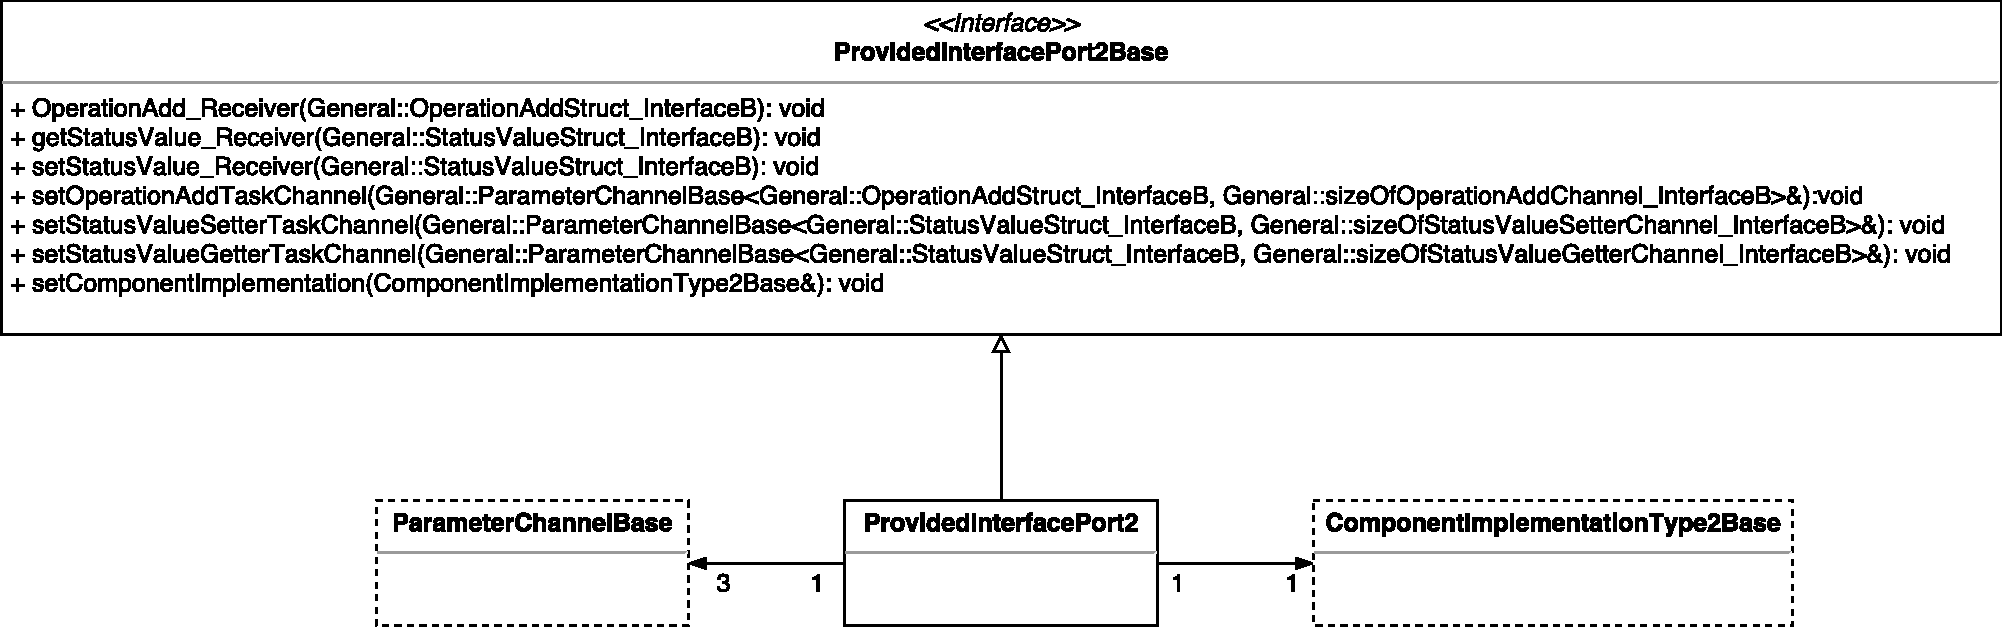
\includegraphics[width=1.0\textwidth]{ProvidedInterfacePort2UML.pdf}
	\caption{UML class diagram representation of \texttt{Provided\allowbreak Interface\allowbreak Port2} for \texttt{Component\allowbreak\_Callee} in the example OBSW model}
	\label{fig: Provided interface port2 UML}
\end{figure}

\begin{figure}[h]
	\centering
	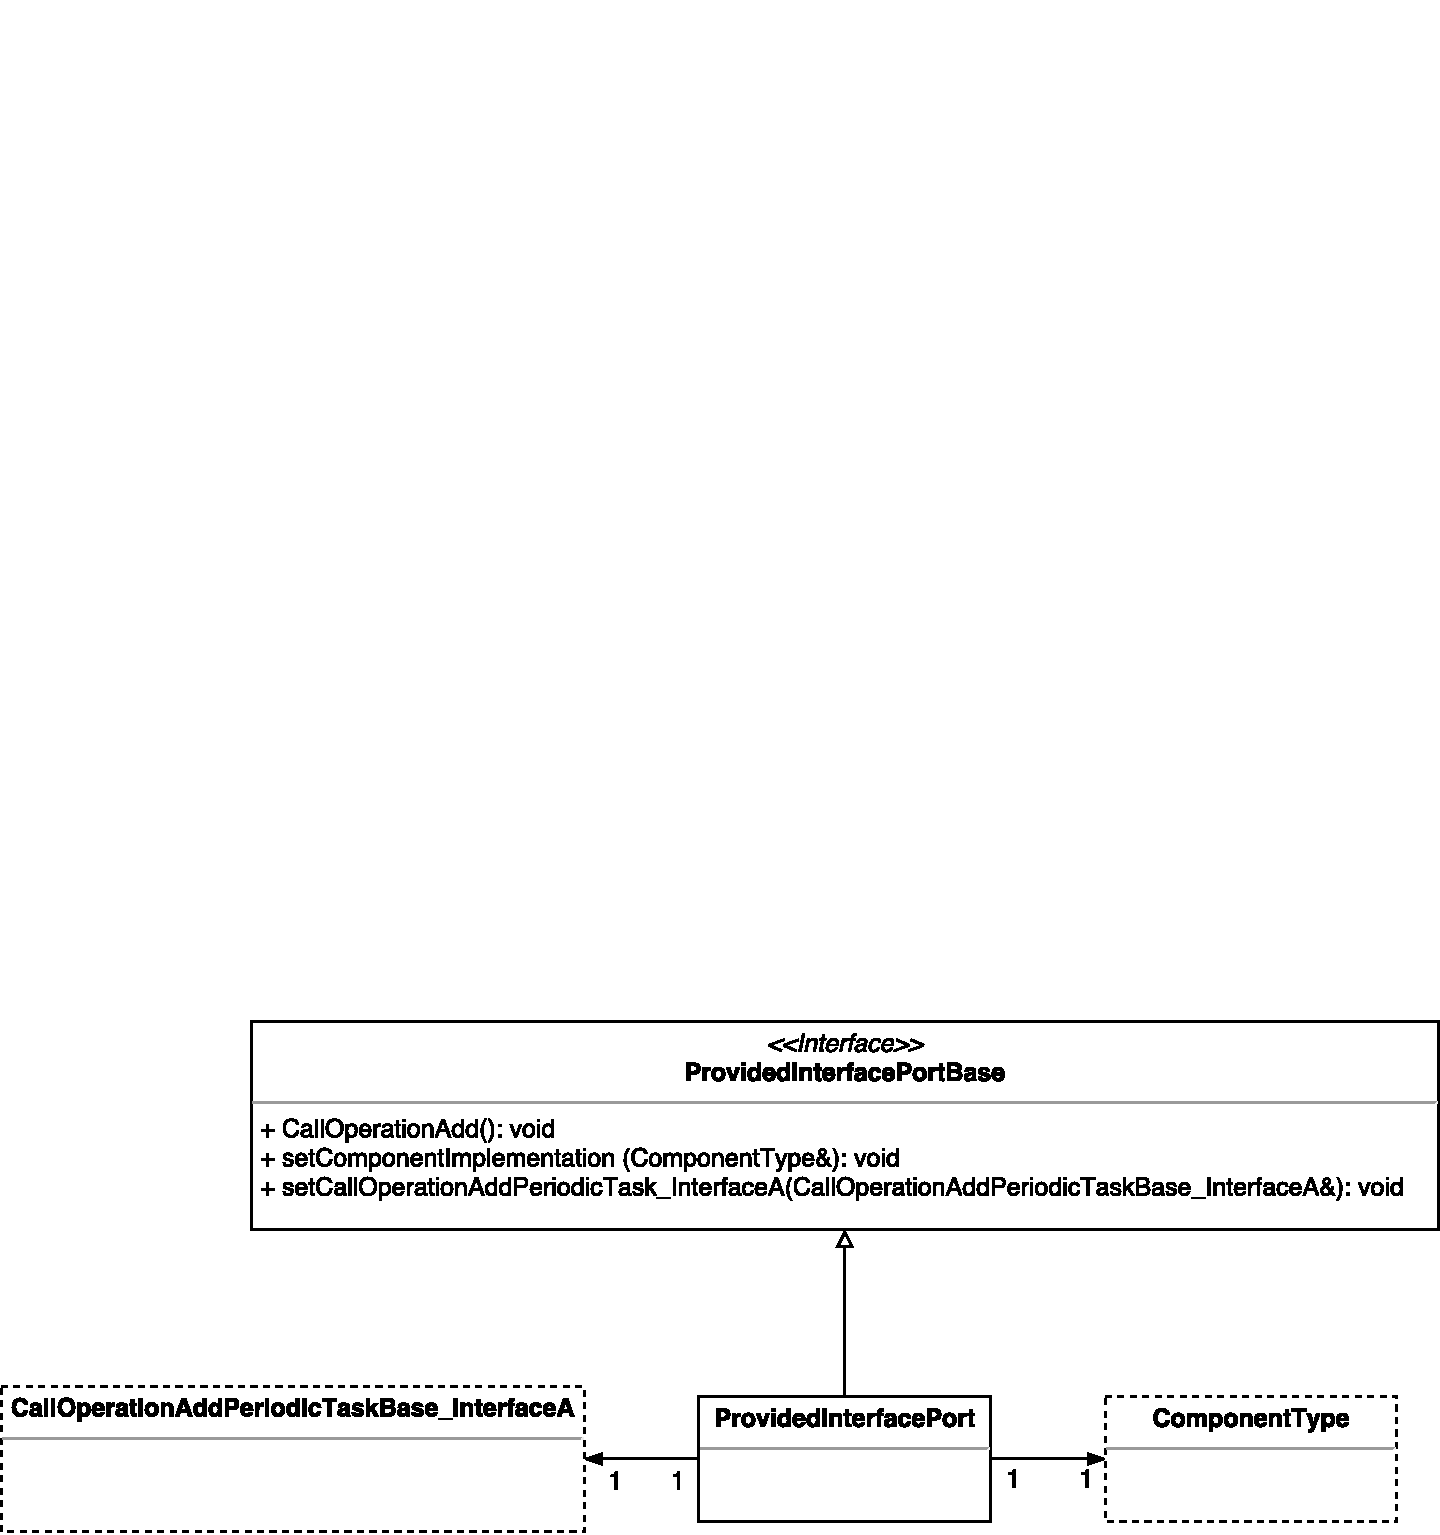
\includegraphics[width=1.0\textwidth]{ProvidedInterfacePortUML.pdf}
	\caption{UML class diagram representation of \texttt{Provided\allowbreak Interface\allowbreak Port} for \texttt{Component\allowbreak\_Caller} in the example OBSW model}
	\label{fig: Provided interface port UML}
\end{figure}   

The concrete implementation for the methods, in case the corresponding operation is requested to be released synchronously, consists of a simple call to the corresponding method in the referenced component implementation base class as shown in code excerpt in \cref{Listing: Provided interface port1 Impl}. If the non-functional property attached with release of the operation on the provided interface side is \texttt{Protected}, then the implementation also includes acquiring and releasing of semaphore associated with the operation as shown in code excerpt in \cref{Listing: Provided interface port1 Impl}. 

\begin{Listing}
\begin{lstlisting}[language=C++]
General::OperationAddReport ProvidedInterfacePort1::OperationAdd (const IntegerType& a,const IntegerType& b,IntegerType& c) {
	General::OperationAddReport_InterfaceB myReport;
	m_myComponent->lockOperationAdd_InterfaceB();
	myReport = m_myComponent->OperationAdd(a,b,c); //Simple method call
	m_myComponent->releaseOperationAdd_InterfaceB();
	return myReport;
}
\end{lstlisting}
\caption{Code excerpt from the generated code for operation \texttt{OperationAdd} access in \texttt{Provided\allowbreak Interface\allowbreak Port1} which is called synchronously and has \texttt{Protected} as a non-functional property attached to it}
\label{Listing: Provided interface port1 Impl}
\end{Listing}

The concrete implementation for the methods, in case the corresponding operation is requested to be released asynchronously, consist of pushing the data structure associated with the operation onto the corresponding task channel as shown in code excerpt in \cref{Listing: Provided interface port2 Impl} . A diagrammatic representation of the push that is required, is already shown in Step 2 of each of these figures \cref{fig: Asynchronous sporadic}, \cref{fig: Asynchronous protected}, \cref{fig: Asynchronous bursty} in the section which deals with the required code archetypes in the programming model for asynchronous release patterns.

\begin{Listing}
\begin{lstlisting}[language=C++]
void ProvidedInterfacePort2::OperationAdd_Receiver (General::OperationAddStruct_InterfaceB myStruct) {
	m_myOperationAddChannel->push(myStruct); //A push onto the task channel
}
\end{lstlisting}
\caption{Code excerpt from the generated code for operation \texttt{OperationAdd} access in \texttt{Provided\allowbreak Interface\allowbreak Port2} which is called asynchronously}
\label{Listing: Provided interface port2 Impl}
\end{Listing}

The concrete implementation for the methods, in case the corresponding operation is requested to be released asynchronously, with non-functional property as \texttt{cyclic} is a simple call to start the task using the reference to the task as shown in the code excerpt in \cref{Listing: Provided interface port Impl}.

\begin{Listing}
\begin{lstlisting}[language=C++]
void ProvidedInterfacePort::CallOperationAdd(void) {
	m_mycallOperationAddTask->startPeriodicTask(); //Method call to start the task
}
\end{lstlisting}
\caption{Code excerpt from the generated code for operation \texttt{CallOperationAdd} in \texttt{Provided\allowbreak Interface\allowbreak Port} which has non-functional property set as \texttt{Cyclic}}
\label{Listing: Provided interface port Impl}
\end{Listing}

\textbf{For our example OBSW model}: The following classes as shown in \cref{fig: Provided interface port1 UML}, \cref{fig: Provided interface port2 UML}, \cref{fig: Provided interface port UML} are defined:
\begin{itemize}
\item \texttt{Provided\allowbreak Interface1\allowbreak Base} abstract base class and its corresponding \texttt{Provided\allowbreak Interface\allowbreak Port1} concrete implementation class
\item \texttt{Provided\allowbreak Interface2\allowbreak Base} abstract base class and its corresponding \texttt{Provided\allowbreak Interface\allowbreak Port2} concrete implementation class
\item \texttt{Provided\allowbreak Interface\allowbreak Port} abstract base class and its corresponding \texttt{Provided\allowbreak Interface\allowbreak Port} concrete implementation class 
\end{itemize} 

All the abstract base classes have pure virtual methods as per the general description given above and they have to be implemented in the corresponding concrete implementation classes. The concrete implementations are in line with the description as in the general case above.

\subsubsection{\textbf{Tasks from the Tasking framework}}
In the discussions about designing a programming model for OSRA in the \cref{chap: Progamming model}, it was clear that the threads of control might contain tasks from the Tasking framework. Each task is mapped to an abstract base class and a concrete implementation class in C++. A task would have instances of the required task inputs, task event as per the required threads of control explained in detail in the chapter on arriving at a programming model for OSRA.

Each task stores a reference to the base class of the component implementation in order to access the services implemented in the respective component implementations.  

\textbf{For our example OBSW model}: The following classes as shown in \cref{fig: Periodic task UML}, \cref{fig: Sporadic task UML}, \cref{fig: Status value getter setter task UML}, \cref{fig: Event receiver task UML} are defined:
\begin{itemize}
\item \texttt{CallOperationAdd\allowbreak Periodic\allowbreak TaskBase\allowbreak \_InterfaceA} abstract base class and \texttt{Call\allowbreak OperationAdd\allowbreak Periodic\allowbreak Task} concrete implementation class, in order to call operation \texttt{Call\allowbreak OperationAdd} in the \texttt{Provided\allowbreak Interface\allowbreak Port} perioidically every 2s
\item \texttt{OperationAdd\allowbreak Sporadic\allowbreak TaskBase\allowbreak \_InterfaceB} abstract base class and a corresponding \texttt{Operation\allowbreak Add\allowbreak Sporadic\allowbreak Task} concrete implementation class, in order to call operation \texttt{Operation\allowbreak Add} in the \texttt{Provided\allowbreak Interface\allowbreak Port2} sporadically with an MIAT of 2s
\item \texttt{StatusValue\allowbreak SetterTaskBase\allowbreak \_InterfaceB} abstract base class and a corresponding \texttt{Status\allowbreak Value\allowbreak Setter\allowbreak Task} concrete implementation class, in order to provide asynchronous access to the setter operation of the interface attribute \texttt{Status\allowbreak Value} in the \texttt{Provided\allowbreak Interface\allowbreak Port2}
\item \texttt{StatusValue\allowbreak SetterTaskBase\allowbreak \_InterfaceB} abstract base class and a corresponding \texttt{Status\allowbreak Value\allowbreak Getter\allowbreak Task} concrete implementation class, in order to provide asynchronous access to the getter operation of the interface attribute \texttt{Status\allowbreak Value} in the \texttt{Provided\allowbreak Interface\allowbreak Port2}
\item \texttt{Failure\allowbreak Event\allowbreak Receiver\allowbreak Task\allowbreak Base} abstract base class and a corresponding \texttt{Failure\allowbreak Event\allowbreak Receiver\allowbreak Task} concrete implementation class, for the reception of \texttt{Failure\allowbreak Event} which are emitted by the \texttt{Component\allowbreak\_Callee} asynchronously and to forward it to \texttt{Component\allowbreak\_Caller} 
\end{itemize} 

\begin{figure}[h]
	\centering
	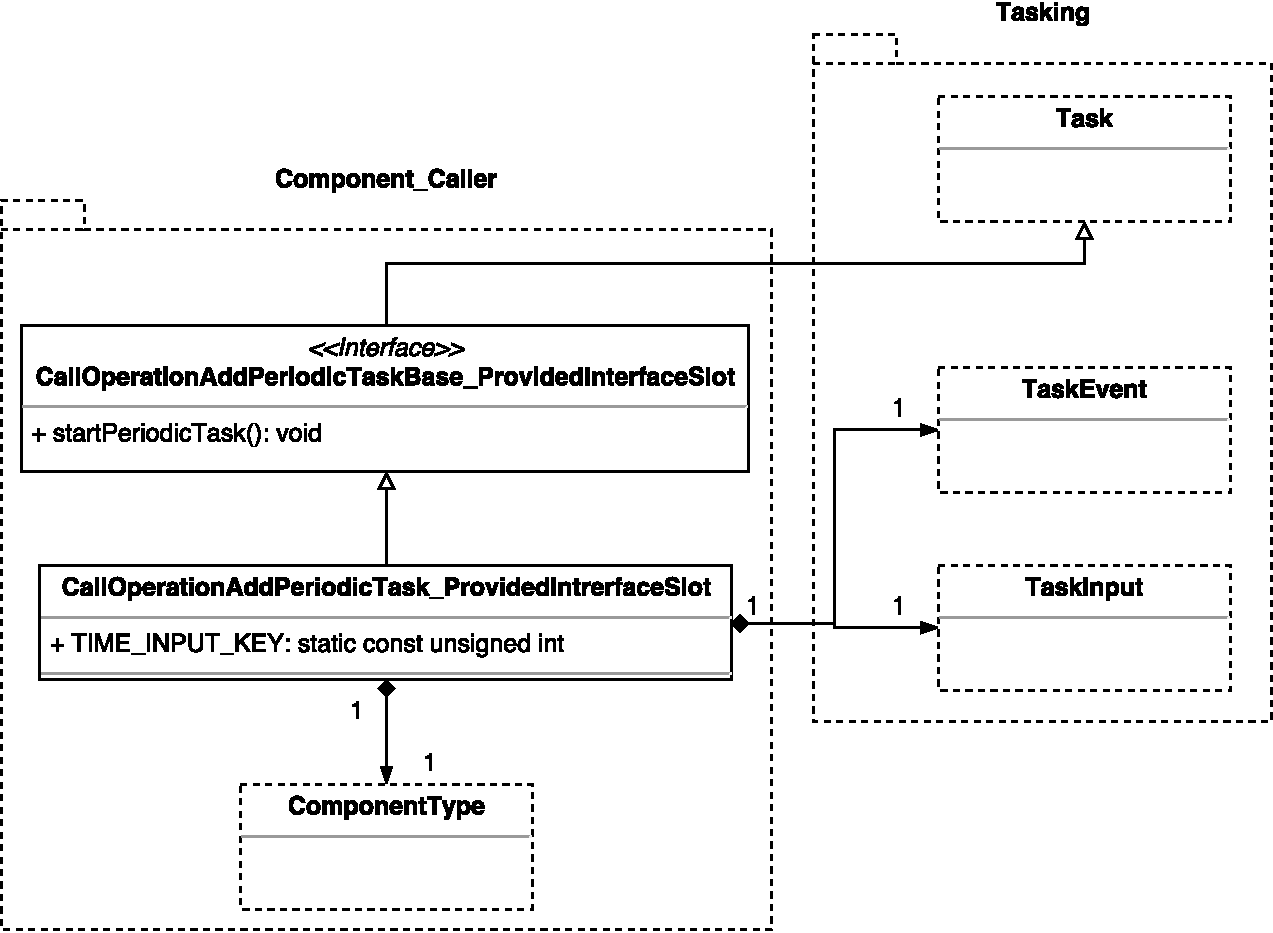
\includegraphics[width=0.8\textwidth]{PeriodicTaskUML.pdf}
	\caption{UML class diagram representation of the task required to call \texttt{CallOperationAdd} in \texttt{Provided\allowbreak Interface\allowbreak Port} perioidcally with a period of 2s in the example OBSW model}
	\label{fig: Periodic task UML}
\end{figure}

\begin{figure}[h]
	\centering
	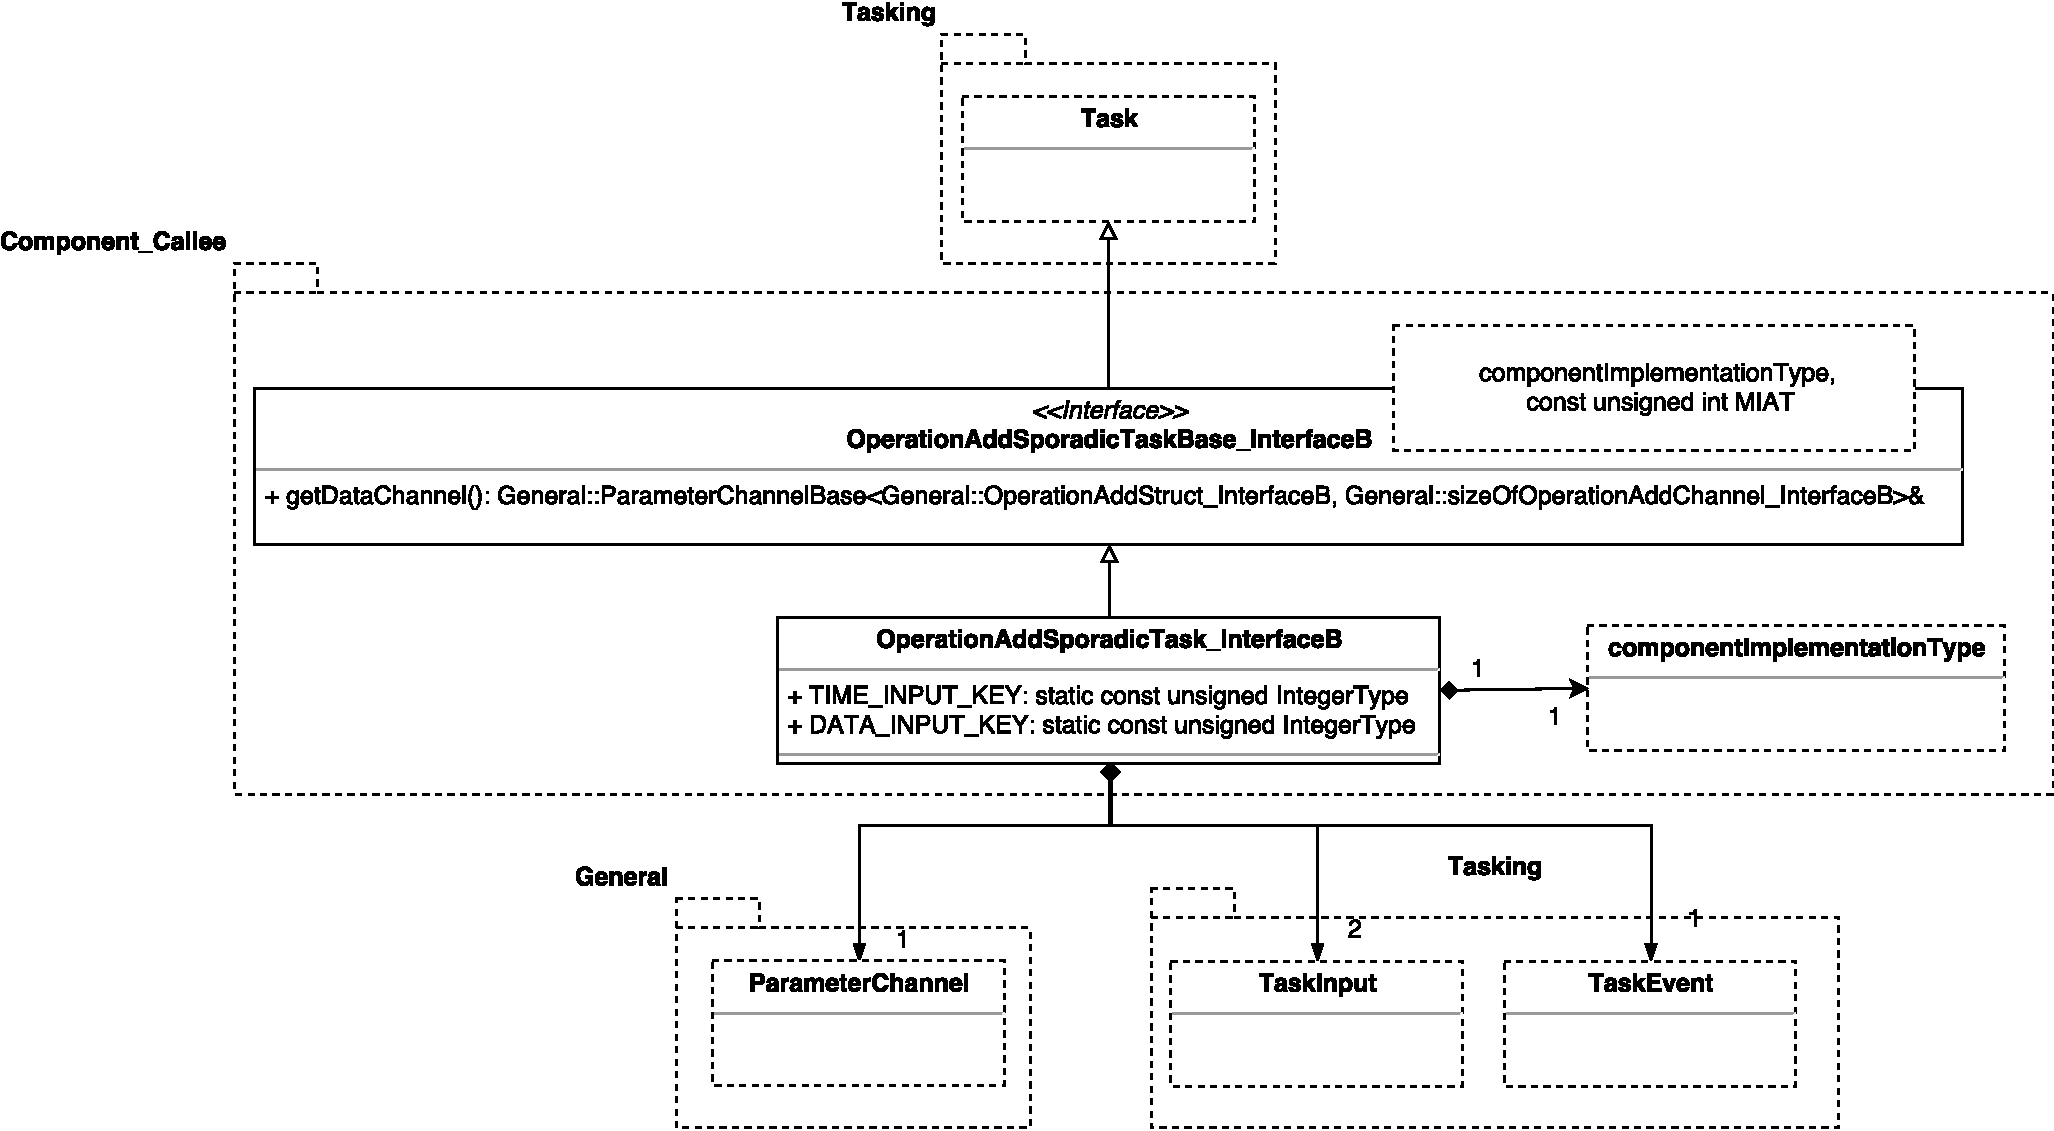
\includegraphics[width=1.0\textwidth]{SporadicTaskUML.pdf}
	\caption{UML class diagram representation of the task required to call \texttt{OperationAdd} in \texttt{Provided\allowbreak Interface\allowbreak Port2} sporadically with a MIAT of 2s in the example OBSW model}
	\label{fig: Sporadic task UML}
\end{figure}

\begin{figure}[h]
	\centering
	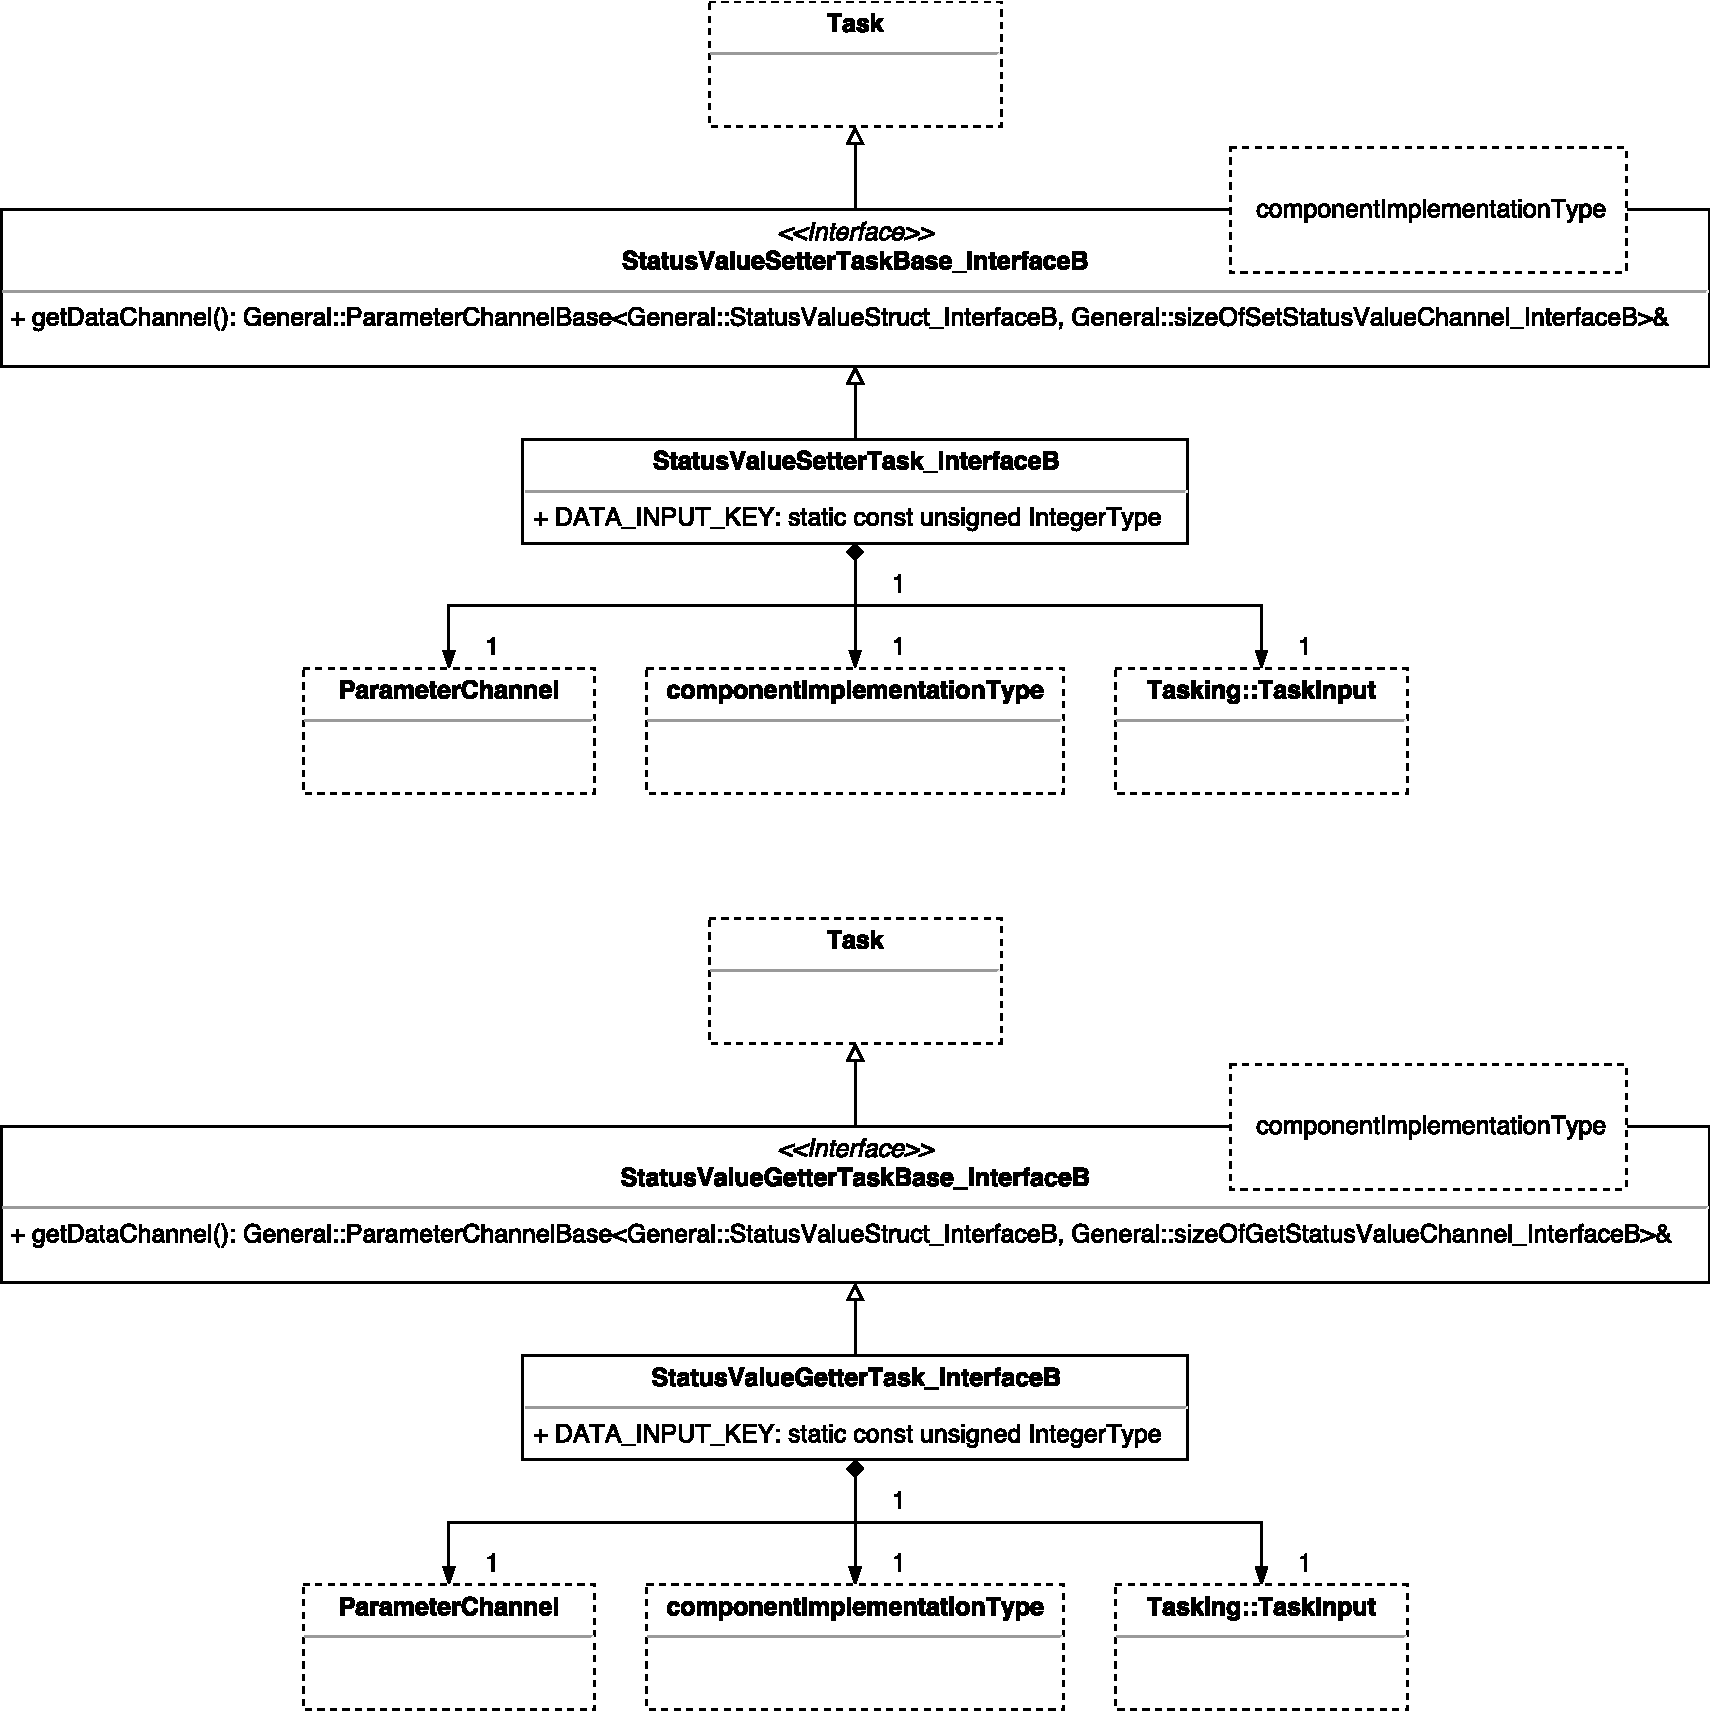
\includegraphics[width=1.0\textwidth]{SetterGetterTaskUML.pdf}
	\caption{UML class diagram representation of the tasks required to set and get the values of the interface attributes asynchronously in \texttt{Provided\allowbreak Interface\allowbreak Port2} in the example OBSW model}
	\label{fig: Status value getter setter task UML}
\end{figure}

\begin{figure}[h]
	\centering
	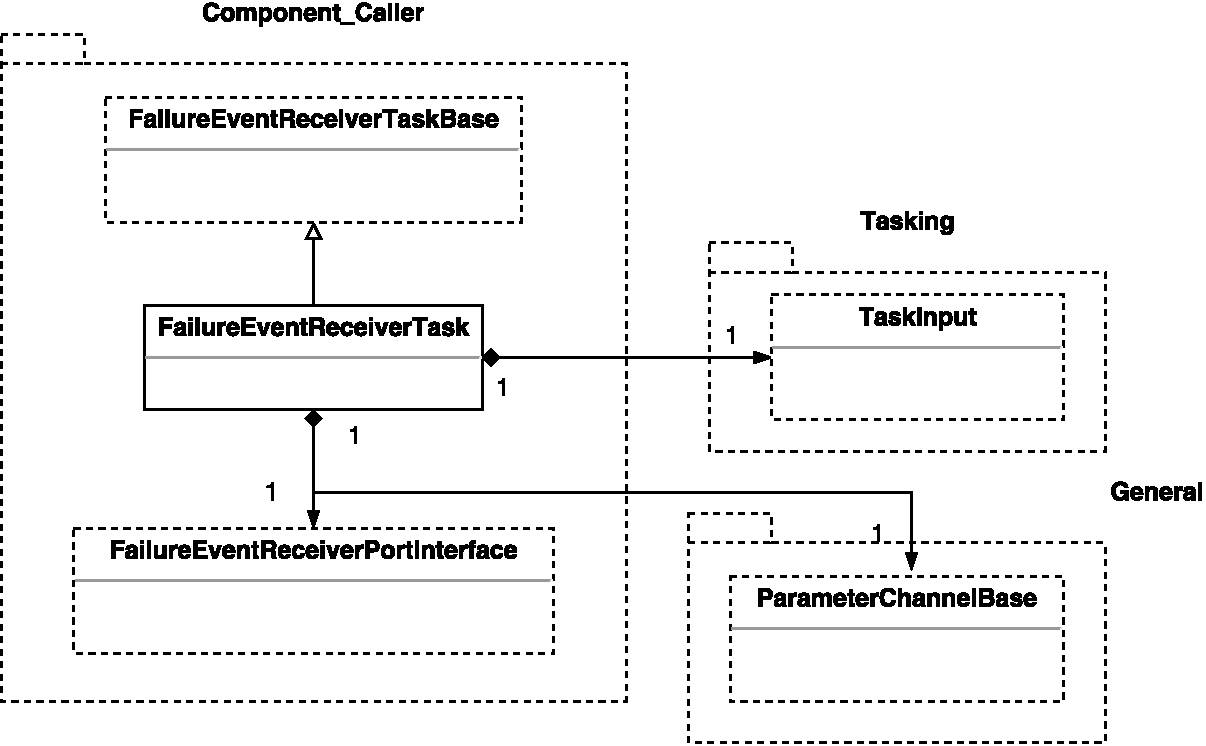
\includegraphics[width=0.8\textwidth]{FailureEventReceiverTaskUML.pdf}
	\caption{UML class diagram representation of the task required for the reception of the \texttt{Failure\allowbreak Event} in the example OBSW model}
	\label{fig: Event receiver task UML}
\end{figure}

\subsubsection{\textbf{Component containers}}
A container of a component can be mapped to a class in C++ as in \cite{EvoRAVCodeAr}. A component container consists of the following things:

\begin{itemize}
\item Instances of required interface ports
\item Instance of component implementation 
\item Instances of tasks which are necessary to handle services which are called asynchronously 
\item Instances of tasks which are necessary to receive asynchronous events
\item Instances of event emitter ports
\end{itemize}

A component container is also responsible for initializing the following:

\begin{itemize}
\item The instantiated component instance by providing references of the event emitter ports
\item The event emitter port by providing reference of the task channel to which the emitter port needs to push the information about the event
\item The provided interface ports by:
\begin{itemize}
\item Triggering the operations in the provided interface ports which have the desired non-function property set as \texttt{cyclic} 	
\item Providing reference of the component instance in order to access the service
\item Providing references of the different task channels they need to push the data structures associated with the operations onto, in order to handle the services which have the interaction kind specifies as \texttt{asynchronous} 
\end{itemize}
\item The instances of tasks with reference of component instance in order to schedule the execution of the services
\item The required interface ports by providing references of:
\begin{itemize}
\item The component instance, in order to initialize the data structures of the operations with correct function wrappers for call-back functions
\item The respective provided interface port each one of them is bound to 
\end{itemize}
\item The event receiver tasks with references of the component instance and the channels which needs to be associated with their respective task inputs      
\end{itemize}

\textbf{For our example OBSW model}: The following classes as shown in \cref{fig: Component container caller UML} and \cref{fig: Component container callee UML} are defined:

\begin{itemize}
\item \texttt{Container} in the namespace \texttt{Component\allowbreak\_Caller} which is the container for the component instance \texttt{Component\allowbreak\_Caller\allowbreak\_impl\allowbreak\_inst} and its provided and required interface slots
\item \texttt{Container} in the namespace \texttt{Component\allowbreak\_Callee} which is the container for the component instance \texttt{Component\allowbreak\_Callee\allowbreak\_impl\allowbreak\_inst} and its provided interface slots 
\end{itemize}

\begin{figure}[h]
	\centering
	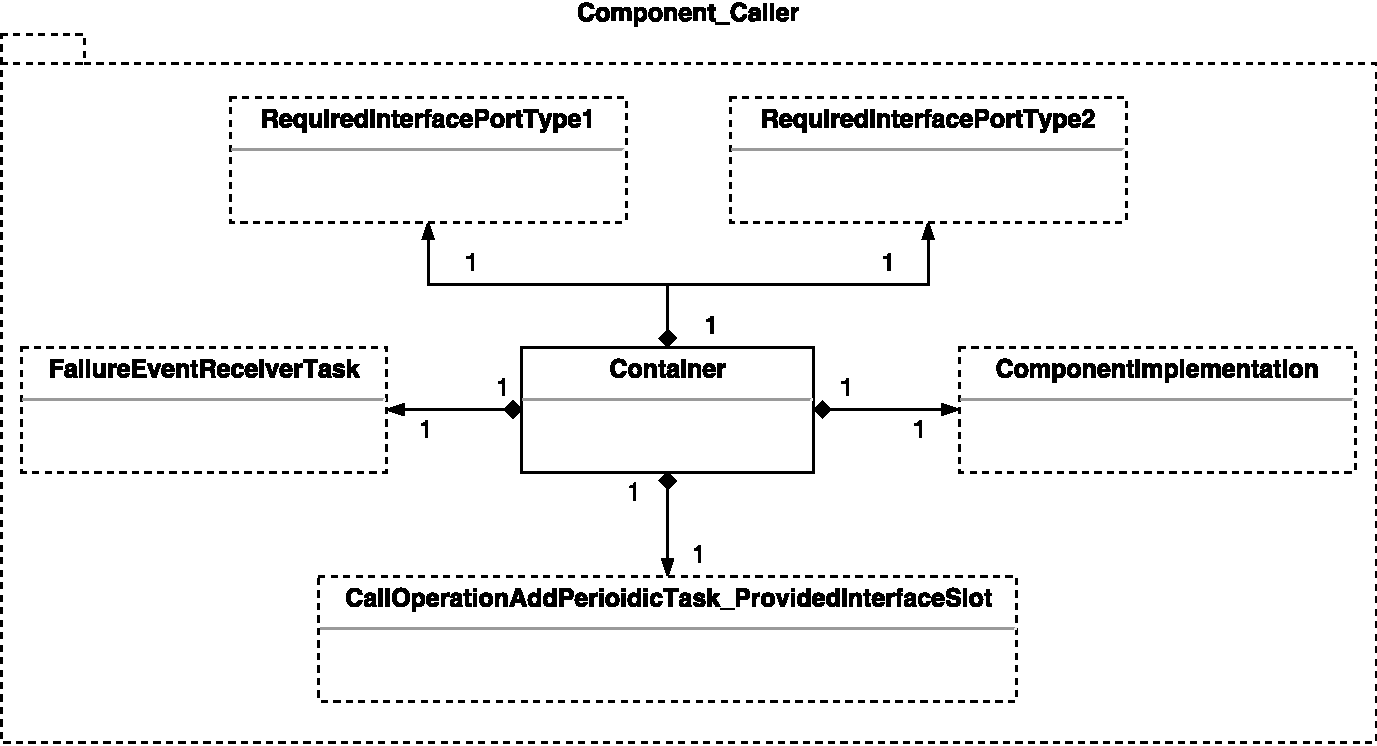
\includegraphics[width=0.8\textwidth]{ComponentContainerCallerUML.pdf}
	\caption{UML class diagram representation of the container for \texttt{Component\allowbreak \_Caller} in the example OBSW model}
	\label{fig: Component container caller UML}
\end{figure}

\begin{figure}[h]
	\centering
	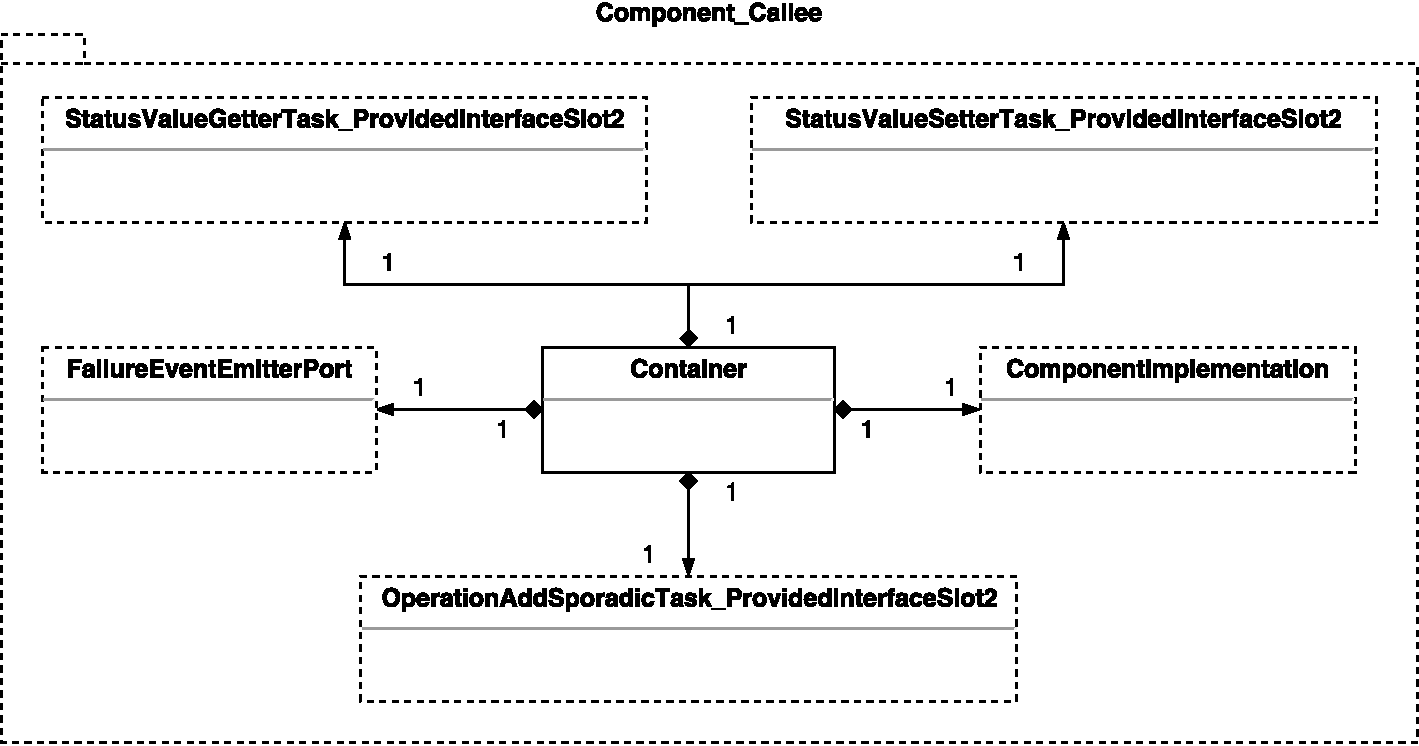
\includegraphics[width=0.8\textwidth]{ComponentContainerCalleeUML.pdf}
	\caption{UML class diagram representation of the container for \texttt{Component\allowbreak \_Callee} in the example OBSW model}
	\label{fig: Component container callee UML}
\end{figure}

Both the containers have instances of different component as explained in the general case and as shown in \cref{fig: Component container caller UML} and \cref{fig: Component container callee UML}. They are responsible for the initialization of different components as explained in the above general description.  

\section{Code generation using Xtend}
\label{section: code generation}
The reference implementation of the OSRA component model consists in a set of .ecore metamodels \cite{SpecMetamodel}. Ecore is an implementation of the EMOF (Essential MOF), the meta-meta language by the OMG for the specification of meta-models \cite{SpecMetamodel}. The main advantage of using Ecore is the ready availability of graphical editors for the specification of metamodels and powerful support provided by the Eclipse Modeling Framework (EMF), which is a framework of the Eclipse development platform that permits to generate a code implementation of the metamodel entities, basic editors for the creation of models conforming to the metamodel under development \cite{SpecMetamodel}. 

It is an implementation decision in this Master thesis to use Xtend for the code generation. Xtend is a general purpose Java-like language that is completely operable with Java \cite{Xtend,XtendDoc}. Xtend has a more concise syntax than Java and provides powerful features such as type inference, extension methods, dispatch methods, an lambda expressions and the all important multiline template expressions, which are useful when writing code generators \cite{Xtend,XtendDoc}. Xtend also provides powerful features that make model visiting and traversing really easy, straightforward, and natural to read and maintain. 

Xtext is an eclipse framework for implementing programming languages and Domain Specific Languages (DSLs) \cite{Xtend}. Xtext helps to implement languages quickly, and most of all, it covers all the aspects of a complete language infrastructure like parser, code generator etc. Xtext uses Google Guice, which is a dependency injection framework to create and call a code generator \cite{Xtend}. The dependency injection pattern basically allows to inject implementation objects into a class hierarchy in a consistent way \cite{InvOfCntrlurl}. The Xtext's generator support can be used in Xtend directly to build code generators for non-Xtext based models, such as the OBSW models constructed using the OSRA component model \cite{CodeGenEclXtend}. 

The tutorial in \cite{CodeGenNonXtext} is used as a base in this Master thesis to construct a code generator for non-Xtext based models using Xtend and also provide a UI integration for the code generator.

\section{Organizing the generated code}
\label{section: Code organization}
As explained in the previous sections, adopting separation of concerns even at the implementation level is one of the primary goals of this chapter and we have successfully achieved it in the discussions on software design for the infrastructural code in \cref{subsection: Software design approach}. 

To further emphasize on separation of concerns at the implementation level, it is necessary to properly sort the generated infrastructure code into a meaningful file structure helping the third party software supplier to separate the automatically generated code from the code that needs to be supplied. This is of prime importance for the third party software supplier to not accidentally lose the implementations in successive code generation cycles. 

The overall idea would be to:
\begin{itemize}
\item Generate two folders per component to clearly separate the infrastructural code entities, at the component type level from the infrastructural code entities at the component instance level 
\begin{itemize}
\item The first folder would hold C++ classes related to its component type, required interface ports, event emitter ports, event receiver ports in the sub-folder named as \texttt{AutogeneratedCode}. It also contains C++ classes related to component implementations and because it is the unit of sub-contract, it is placed in a separate sub-folder named as \texttt{UserCode}. The third-party software supplier can alter the code in this folder safely without the fear of the code being overwritten by successive code generation cycles. Care is taken in the code generator to generate the classes in these files only once  
\item The second folder would hold the C++ classes related to provided interface ports, component containers in the sub-folder named as \texttt{AutogeneratedCode}. As already explained the component container class for a component would contain provided and required interface slots, component instance   
\end{itemize} 
\item The folder named as \texttt{Datatypes\allowbreak Interfaces\allowbreak EventsAnd\allowbreak Exceptions} would hold C++ classes related to the data types, exceptions, events, parameter channel and their corresponding parameter queues 
\end{itemize}

Considering our running example, the folder structure is as explained below:

All the data types, event types, interfaces, exception types that are used in the example are stored along with the parameter channel and parameter queue as shown below:

\newpage 

\dirtree{%
.1 src-gen.
.2 DatatypesInterfacesEventsAndExceptions.
.3 include.
.4 Datatypes.h.
.4 Exceptions.h.
.4 FailureEvent.h.
.4 InterfaceA.h.
.4 InterfaceB.h.
.4 ParameterChannel.h.
.4 ParameterQueue.h.
}

All the constituents of the \texttt{Component\_Callee} are arranged as shown below:

\dirtree{%
.1 src-gen.
.2 Component\_Callee.
.3 AutogeneratedCode.
.4 include.
.5 ComponentType\_Callee.h.
.5 EventEmitterPorts\_Callee.h.h.
.4 src.
.5 ComponentType\_Callee.cpp.
.5 EventEmitterPorts\_Callee.cpp.
.3 UserCode.
.4 include.
.5 ComponentImplementation\_Callee.h.
.4 src.
.5 ComponentImplementation\_Callee.cpp.
.2 Component\_Callee\_Instance.
.3 AutogeneratedCode.
.4 include.
.5 ProvidedInterfacePorts\_Callee.h.
.5 ComponentContainer\_Callee.h.
.4 src.
.5 ProvidedInterfacePorts\_Callee.cpp.
.5 ComponentContainer\_Callee.cpp.
}

\newpage

All the constituents of the \texttt{Component\_Caller} are arranged as shown below:
\dirtree{%
	.1 src-gen.
	.2 Component\_Caller.
	.3 AutogeneratedCode.
	.4 include.
	.5 ComponentType\_Caller.h.
	.5 EventReceiverPorts\_Caller.h.
	.5 RequiredInterfacePorts\_Caller.h.
	.4 src.
	.5 ComponentType\_Caller.cpp.
	.5 EventReceiverPorts\_Caller.cpp.
	.5 RequiredInterfacePorts\_Caller.cpp.
	.3 UserCode.
	.4 include.
	.5 ComponentImplementation\_Caller.h.
	.4 src.
	.5 ComponentImplementation\_Caller.cpp.
	.2 Component\_Caller\_Instance.
	.3 AutogeneratedCode.
	.4 include.
	.5 ProvidedInterfacePorts\_Caller.h.
	.5 ComponentContainer\_Caller.h.
	.4 src.
	.5 ProvidedInterfacePorts\_Caller.cpp.
	.5 ComponentContainer\_Caller.cpp.
}
  



 

   

 


 
   



 


 

% !TeX spellcheck = en_US

\chapter{Results and Conclusions}
\label{chap:conclusion}

\section{Discussion}
As a part of this Master thesis, 
\begin{itemize}
\item A choice is made to use the Tasking framework as a computational model so that the OSRA component model statically binds to Tasking framework which formally defines the computational entities and the rules which govern their usage 
\item A reference programming model is decided upon that enforces the analysis assumptions and which permits to express exclusively the semantics imposed by the analysis theory and which conveys the implementations of the desired non-functional properties using the primitives from the Tasking framework
\item Different corner cases which might arise during the construction of an OBSW model using the OSRA component model are identified 
\item An overall software design approach for the generated infrastructure code of the OBSW models is presented and a mapping of the OBSW model design entities to the infrastructural code entities is presented. The generated code would then have all the good characteristics of a software as listed in \cref{subsection: Software design approach} 
\item A code generator is implemented, using which the generation of the entire non-functional code i.e., the code for handling the concurrency and interaction requirements for communication between components and generation of component containers and component connectors can be automated. The code generator uses the already tried and tested Tasking framework as the platform and bases the generated code on it. The advantage of this is that it eases the model-to-code transformation step 
\item The implemented code generator is tested for multiple OBSW models as shown in \cref{chap: Extra examples} which capture the different corner cases identified
\item For the simple OBSW model example which was introduced in \cref{chap: Code generation}, a set of unit test cases are written using Gtest and Gmock frameworks and the test coverage reports are generated
\end{itemize}

The following results were obtained 
\begin{itemize}
\item  The implemented code generator successfully generates the infrastructural code entities for all the example OBSW models listed in \cref{chap: Code generation} and in \cref{chap: Extra examples}. The generated code in all cases is successfully compiled along with Tasking framework using GCC C++ compiler conforming to the C++11 standard for the Linux platform
\item The test coverage reports generated for the unit tests written for the simple OBSW example are analyzed. The results show that the testability factor of the generated code is high and the infrastructural code entities can be efficiently tested      
\end{itemize}

\section{Identified shortcomings of Tasking framework}
During the course of the Master thesis, the following shortcomings of the current version of Tasking framework, which is chosen as a computational model for this Master thesis are identified:
\begin{itemize}
\item Tasks from Tasking framework are used in various threads of control as explained in \cref{chap: Progamming model}. At the heart of the Tasking framework is a scheduler which schedules tasks based on priorities and these tasks are non-preemptible at the moment \cite{TaskFr}. This is one of the critical shortcomings in the current version of the Tasking framework as it makes the generated software code which is based on Tasking framework not suitable for hard real-time systems \cite{TempIsolation}. Time-monitoring architectures such as Server-based architecture or Priority-Band architectures listed in \cite{TempIsolation} are the ways to go ahead in case making the code making use of the Tasking framework truly real-time capable. These architectures help in providing isolation of applications i.e., tasks (at least) along three orthogonal dimensional axes: time, space and communication
\item In the current version of the Tasking framework there is no possibility to measure the run-time of the tasks and monitor deadline violations which are mostly caused by WCET overruns of either the task at hand or a higher priority task. This limits the extent of property preservation in the model-to-code transformation step \cite{TempIsolation}. It is of very high importance that the system properties asserted during the analysis and the assumptions made for the analysis to hold are preserved across implementation and execution \cite{EvoRAVCodeAr}\cite{TempIsolation}
\item It is also not possible to measure the execution time of a group tasks which are associated to the single time budget so that the Group Budget is accounted for their collective execution time. This incapability makes the adoption of Server-based architecture in the Tasking framework more difficult
\item In line with the inability to measure the run-time of the tasks from the Tasking framework, Tasking Framework also does not provide any constructs for at least coarse-grained fault detection and fault handling in case of deadline misses
\item 
\end{itemize}

\section{Future Work}
As an enhancement to the current work, it is possible to extend this Master thesis  
\label{section: Future work}


%
%
%\renewcommand{\appendixtocname}{Anhang}
%\renewcommand{\appendixname}{Anhang}
%\renewcommand{\appendixpagename}{Anhang}
\appendix
$  $% !TeX spellcheck = de_DE
%Die Angabe des schlauen Spruchs auf diesem Wege funtioniert nur,
%wenn keine Änderung des Kapitels mittels den in preambel/chapterheads.tex
%vorgeschlagenen Möglichkeiten durchgeführt wurde.
\setchapterpreamble[u]{%
\dictum[Albert Einstein]{Probleme kann man niemals mit derselben Denkweise lösen, durch die sie entstanden sind.}
}
\chapter{LaTeX-Tipps}
\label{chap:latextipps}

\section{File-Encoding und Unterstützung von Umlauten}
\label{sec:firstsectioninlatexhints}
Die Vorlage wurde 2010 auf UTF-8 umgestellt.
Alle neueren Editoren sollten damit keine Schwierigkeiten haben.

\section{Zitate}
Referenzen werden mittels \texttt{\textbackslash cite[key]} gesetzt.
Beispiel: \cite{WSPA} oder mit Autorenangabe: \citet{WSPA}.

Der folgende Satz demonstriert \begin{inparaenum}[1.]
\item die Großschreibung von Autorennamen am Satzanfang,
\item die richtige Zitation unter Verwendung von Autorennamen und der Referenz,
\item dass die Autorennamen ein Hyperlink auf das Literaturverzeichnis sind sowie
\item dass in dem Literaturverzeichnis der Namenspräfix \enquote{van der} von \enquote{Wil M.\,P.\ van der Aalst} steht.
\end{inparaenum}
\Citet{RVvdA2016} präsentieren eine Studie über die Effektivität von Workflow-Management-Systemen.

Der folgende Satz demonstriert, dass man mittels \texttt{label} in einem Bibliopgrahie"=Eintrag den Textteil des generierten Labels überschreiben kann, aber das Jahr und die Eindeutigkeit noch von biber generiert wird.
Die Apache ODE Engine \cite{ApacheODE} ist eine Workflow-Maschine, die BPEL-Prozesse zuverlässig ausführt.

Wörter am besten mittels \texttt{\textbackslash enquote\{...\}} \enquote{einschließen}, dann werden die richtigen Anführungszeichen verwendet.

Beim Erstellen der Bibtex-Datei wird empfohlen darauf zu achten, dass die DOI aufgeführt wird.

\section{Mathematische Formeln}
\label{sec:mf}
Mathematische Formeln kann man $so$ setzen. \texttt{symbols-a4.pdf} (zu finden auf \url{http://www.ctan.org/tex-archive/info/symbols/comprehensive/symbols-a4.pdf}) enthält eine Liste der unter LaTeX direkt verfügbaren Symbole.
Z.\,B.\ $\mathbb{N}$ für die Menge der natürlichen Zahlen.
Für eine vollständige Dokumentation für mathematischen Formelsatz sollte die Dokumentation zu \texttt{amsmath}, \url{ftp://ftp.ams.org/pub/tex/doc/amsmath/} gelesen werden.

Folgende Gleichung erhält keine Nummer, da \texttt{\textbackslash equation*} verwendet wurde.
\begin{equation*}
x = y
\end{equation*}

Die Gleichung~\ref{eq:test} erhält eine Nummer:
\begin{equation}
\label{eq:test}
x = y
\end{equation}

Eine ausführliche Anleitung zum Mathematikmodus von LaTeX findet sich in \url{http://www.ctan.org/tex-archive/help/Catalogue/entries/voss-mathmode.html}.

\section{Quellcode}
\Cref{lst:ListingANDlstlisting} zeigt, wie man Programmlistings einbindet.
Mittels \texttt{\textbackslash lstinputlisting} kann man den Inhalt direkt aus Dateien lesen.

%Listing-Umgebung wurde durch \newfloat{Listing} definiert
\begin{Listing}
\begin{lstlisting}
<listing name="second sample">
  <content>not interesting</content>
</listing>
\end{lstlisting}
\caption{lstlisting in einer Listings-Umgebung, damit das Listing durch Balken abgetrennt ist}
\label{lst:ListingANDlstlisting}
\end{Listing}

Quellcode im \lstinline|<listing />| ist auch möglich.

\section{Abbildungen}

Die \cref{fig:chor1} und \ref{fig:chor2} sind für das Verständnis dieses Dokuments wichtig.
Im Anhang zeigt \vref{fig:AnhangsChor} erneut die komplette Choreographie.

%Die Parameter in eckigen Klammern sind optionale Parameter - z.B. [htb!]
%htb! bedeutet: "Liebes LaTeX, bitte platziere diese Abbildung zuerst hier ("_h_ere"). Falls das nicht funktioniert, dann bitte oben auf der Seite ("_t_op"). Und falls das nicht geht, bitte unten auf der Seite ("_b_ottom"). Und bitte, bitte bevorzuge hier und oben, auch wenn's net so optimal aussieht ("!")
%Diese sollten nach Möglichkeit NICHT verwendet werden. LaTeX's Algorithmus für das Platzieren der Gleitumgebung ist schon sehr gut!
\begin{figure}
  \centering
  \includegraphics[width=\textwidth]{choreography.pdf}
  \caption{Beispiel-Choreographie}
  \label{fig:chor1}
\end{figure}

\begin{figure}
  \centering
  \includegraphics[width=.8\textwidth]{choreography.pdf}
  \caption[Beispiel-Choreographie]{Die Beispiel-Choreographie. Nun etwas kleiner, damit \texttt{\textbackslash textwidth} demonstriert wird. Und auch die Verwendung von alternativen Bildunterschriften für das Verzeichnis der Abbildungen. Letzteres ist allerdings nur Bedingt zu empfehlen, denn wer liest schon so viel Text unter einem Bild? Oder ist es einfach nur Stilsache?}
  \label{fig:chor2}
\end{figure}


\begin{figure}
  \centering
    \subfloat[]{\includegraphics[width=0.3\textwidth]{choreography.pdf} \label{fig:subfigA}}
    \subfloat[]{\includegraphics[width=0.3\textwidth]{choreography.pdf} \label{fig:subfigB}}
		\subfloat[Subcaption if needed]{\includegraphics[width=0.3\textwidth]{choreography.pdf} \label{fig:subfigC}}
	\caption{Beispiel um 3 Abbildung nebeneinader zu stellen nur jedes einzeln referenzieren zu können. Abbildung~\ref{fig:subfigB}
 ist die mittlere Abbildung.}
\label{fig:subfig_example}
\end{figure}

Das SVG in \cref{fig:directSVG} ist direkt eingebunden, während der Text im SVG in \cref{fig:latexSVG} mittels pdflatex gesetzt ist.
\todo{Falls man die Graphiken sehen möchte, muss inkscape im PATH sein und im Tex-Quelltext \texttt{\textbackslash{}iffalse} und \texttt{\textbackslash{}iftrue} auskommentiert sein.}

\iffalse % <-- Das hier wegnehmen, falls inkscape im Pfad ist
\begin{figure}
\centering
\includegraphics{svgexample.svg}
\caption{SVG direkt eingebunden}
\label{fig:directSVG}
\end{figure}

\begin{figure}
\centering
\def\svgwidth{.4\textwidth}
\includesvg{svgexample}
\caption{Text im SVG mittels \LaTeX{} gesetzt}
\label{fig:latexSVG}
\end{figure}
\fi % <-- Das hier wegnehmen, falls inkscape im Pfad ist

\section{Tabellen}

\cref{tab:Ergebnisse} zeigt Ergebnisse und die \cref{tab:Ergebnisse} zeigt wie numerische Daten in einer Tabelle representiert werden können.
\begin{table}
  \centering
  \begin{tabular}{ccc}
  \toprule
  \multicolumn{2}{c}{\textbf{zusammengefasst}} & \textbf{Titel} \\ \midrule
  Tabelle & wie & in \\
  \url{tabsatz.pdf}& empfohlen & gesetzt\\

  \multirow{2}{*}{Beispiel} & \multicolumn{2}{c}{ein schönes Beispiel}\\
   & \multicolumn{2}{c}{für die Verwendung von \enquote{multirow}}\\
  \bottomrule
  \end{tabular}
  \caption[Beispieltabelle]{Beispieltabelle -- siehe \url{http://www.ctan.org/tex-archive/info/german/tabsatz/}}
  \label{tab:Ergebnisse}
\end{table}

\begin{table}
	\centering
	\begin{tabular}{l *{8}{d{3.2}}}
		\toprule
						
			   & \multicolumn{2}{c}{\textbf{Parameter 1}} & \multicolumn{2}{c}{\textbf{Parameter 2}} & \multicolumn{2}{c}{\textbf{Parameter 3}} & \multicolumn{2}{c}{\textbf{Parameter 4}} \\
			\cmidrule(r){2-3}\cmidrule(lr){4-5}\cmidrule(lr){6-7}\cmidrule(l){8-9}
			
			\textbf{Bedingungen} & \multicolumn{1}{c}{\textbf{M}} & \multicolumn{1}{c}{\textbf{SD}} & \multicolumn{1}{c}{\textbf{M}} & \multicolumn{1}{c}{\textbf{SD}} & \multicolumn{1}{c}{\textbf{M}} & \multicolumn{1}{c}{\textbf{SD}} & \multicolumn{1}{c}{\textbf{M}} & \multicolumn{1}{c}{\textbf{SD}}\\
			\midrule
			
			W & 1.1 & 5.55 & 6.66 & .01 &  &  &  & \\
			X & 22.22 & 0.0 & 77.5 & .1 &  &  &  & \\
			Y & 333.3 & .1 & 11.11 & .05 &  &  &  & \\
			Z & 4444.44 & 77.77 & 14.06 & .3 &  &  &  & \\
		\bottomrule 
	\end{tabular}
	
	\caption{Beispieltabelle f\"{u}r 4 Bedingungen (W-Z) mit jeweils 4 Parameters mit (M und SD). Hinweiß: immer die selbe anzahl an Nachkommastellen angeben.}
	\label{tab:Werte}
\end{table}

\section{Pseudocode}
\Cref{alg:sample} zeigt einen Beispielalgorithmus.
\begin{Algorithmus} %Die Umgebung nur benutzen, wenn man den Algorithmus ähnlich wie Graphiken von TeX platzieren lassen möchte
\caption{Sample algorithm}
\label{alg:sample}
\begin{algorithmic}
\Procedure{Sample}{$a$,$v_e$}
\State $\mathsf{parentHandled} \gets (a = \mathsf{process}) \lor \mathsf{visited}(a'), (a',c,a) \in \mathsf{HR}$
\State \Comment $(a',c'a) \in \mathsf{HR}$ denotes that $a'$ is the parent of $a$
\If{$\mathsf{parentHandled}\,\land(\mathcal{L}_\mathit{in}(a)=\emptyset\,\lor\,\forall l \in \mathcal{L}_\mathit{in}(a): \mathsf{visited}(l))$}
\State $\mathsf{visited}(a) \gets \text{true}$
\State $\mathsf{writes}_\circ(a,v_e) \gets
\begin{cases}
\mathsf{joinLinks}(a,v_e) & \abs{\mathcal{L}_\mathit{in}(a)} > 0\\
\mathsf{writes}_\circ(p,v_e)
& \exists p: (p,c,a) \in \mathsf{HR}\\
(\emptyset, \emptyset, \emptyset, false) & \text{otherwise}
\end{cases}
$
\If{$a\in\mathcal{A}_\mathit{basic}$}
  \State \Call{HandleBasicActivity}{$a$,$v_e$}
\ElsIf{$a\in\mathcal{A}_\mathit{flow}$}
  \State \Call{HandleFlow}{$a$,$v_e$}
\ElsIf{$a = \mathsf{process}$} \Comment Directly handle the contained activity
  \State \Call{HandleActivity}{$a'$,$v_e$}, $(a,\bot,a') \in \mathsf{HR}$
  \State $\mathsf{writes}_\bullet(a) \gets \mathsf{writes}_\bullet(a')$
\EndIf
\ForAll{$l \in \mathcal{L}_\mathit{out}(a)$}
  \State \Call{HandleLink}{$l$,$v_e$}
\EndFor
\EndIf
\EndProcedure
\end{algorithmic}
\end{Algorithmus}

\clearpage
Und wer einen Algorithmus schreiben möchte, der über mehrere Seiten geht, der kann das nur mit folgendem \textbf{üblen} Hack tun:

{
\begin{minipage}{\textwidth}
\hrule height .8pt width\textwidth
\vskip.3em%\vskip\abovecaptionskip\relax
\stepcounter{Algorithmus}
\addcontentsline{alg}{Algorithmus}{\protect\numberline{\theAlgorithmus}{\ignorespaces Description \relax}}
\noindent\textbf{Algorithmus \theAlgorithmus} Description
%\stepcounter{algorithm}
%\addcontentsline{alg}{Algorithmus}{\thealgorithm{}\hskip0em Description}
%\textbf{Algorithmus \thealgorithm} Description
\vskip.3em%\vskip\belowcaptionskip\relax
\hrule height .5pt width\textwidth
\end{minipage}
%without the following line, the text is nerer at the rule
\vskip-.3em
%
code goes here\\
test2\\
%
\vskip-.7em
\hrule height .5pt width\textwidth
}


\section{Abkürzungen}

Beim ersten Durchlaf betrug die \ac{FR} 5. Beim zweiten Durchlauf war die \ac{FR} 3.

Mit \verb+\ac{...}+ können Abkürungen eingebaut werden, beim ersten aufrufen wird die lange Form eingesetzt. Beim wiederholten Verwenden von \verb+\ac{...}+ wird automatisch die kurz Form angezeigt. Außerdem wird die Abkürzung automatisch in die Abkürzungsliste eingefügt.

Definiert werden Abkürzungen in der Datei \textit{ausarbeitung.tex} im Abschnitt '\%\%\% acro' mithilfe von \verb+\DeclareAcronym{...}{...}+.

Mehr infos unter: \url{http://mirror.hmc.edu/ctan/macros/latex/contrib/acro/acro_en.pdf}

\section{Verweise}
Für weit entfernte Abschnitte ist \enquote{varioref} zu empfehlen:
\enquote{Siehe \vref{sec:mf}}.
Das Kommando \texttt{\textbackslash{}vref} funktioniert ähnlich wie \texttt{\textbackslash{}cref} mit dem Unterschied, dass zusätzlich ein Verweis auf die Seite hinzugefügt wird.
\texttt{vref}: \enquote{\vref{sec:firstsectioninlatexhints}}, \texttt{cref}: \enquote{\cref{sec:firstsectioninlatexhints}}, \texttt{ref}: \enquote{\ref{sec:firstsectioninlatexhints}}.

Falls \enquote{varioref} Schwierigkeiten macht, dann kann man stattdessen \enquote{cref} verwenden.
Dies erzeugt auch das Wort \enquote{Abschnitt} automatisch: \cref{sec:mf}.
Das geht auch für Abbildungen usw.
Im Englischen bitte \verb1\Cref{...}1 (mit großen \enquote{C} am Anfang) verwenden.


%Mit MiKTeX Installation ab dem 2012-01-16 nicht mehr nötig
%Falls ein Abschnitt länger als eine Seite wird und man mittels \texttt{\textbackslash{}vref} auf eine konkrete Stelle in der Section
%verweisen möchte, dann sollte man \texttt{\textbackslash{}phantomsection} verwenden und dann wird
%auch bei \texttt{vref} die richtige Seite angeben.

%%The link location will be placed on the line below.
%%Tipp von http://en.wikibooks.org/wiki/LaTeX/Labels_and_Cross-referencing#The_hyperref_package_and_.5Cphantomsection
%\phantomsection
%\label{alabel}
%Das Beispiel für \texttt{\textbackslash{}phantomsection} bitte im \LaTeX{}-Quellcode anschauen.

%Hier das Beispiel: Siehe Abschnitt \vref{hack1} und Abschnitt \vref{hack2}.

\section{Definitionen}
\begin{definition}[Title]
\label{def:def1}
Definition Text
\end{definition}

\Cref{def:def1} zeigt \ldots

\section{Verschiedenes}
\label{sec:diff}
\ifdeutsch
Ziffern (123\,654\,789) werden schön gesetzt.
Entweder in einer Linie oder als Minuskel-Ziffern.
Letzteres erreicht man durch den Parameter \texttt{osf} bei dem Paket \texttt{libertine} bzw.\ \texttt{mathpazo} in \texttt{fonts.tex}.
\fi

\textsc{Kapitälchen} werden schön gesperrt...

\begin{compactenum}[I.]
\item Man kann auch die Nummerierung dank paralist kompakt halten
\item und auf eine andere Nummerierung umstellen
\end{compactenum}

\section{Weitere Illustrationen}
Abbildungen~\ref{fig:AnhangsChor} und~\ref{fig:AnhangsChor2} zeigen zwei Choreographien, die den
Sachverhalt weiter erläutern sollen. Die zweite Abbildung ist um 90 Grad gedreht, um das Paket
\texttt{rotating} zu demonstrieren.

\begin{figure}
  \centering
  \includegraphics[width=\textwidth]{choreography.pdf}
  \caption{Beispiel-Choreographie I}
  \label{fig:AnhangsChor}
\end{figure}

\begin{landscape}
  %sidewaysfigure
  \begin{figure}
    \centering
    \includegraphics[width=\textwidth]{choreography.pdf}
    \caption{Beispiel-Choreographie II}
    \label{fig:AnhangsChor2}
  \end{figure}
\end{landscape}

\clearpage
%hint by http://tex.stackexchange.com/a/3265/9075
%other option is to use changepage according to http://tex.stackexchange.com/a/2639/9075. This, however, has issues with landscape
\thispagestyle{empty}

\savegeometry{koma}

%If you only have height problems, this is not needed at all
\addtolength{\textwidth}{2cm}
\addtolength{\evensidemargin}{-1cm}

\begin{landscape}
  %sidewaysfigure
  \begin{figure}
    \centerline{\includegraphics[width=0.9\paperheight]{choreography.pdf}}
    \caption{Beispiel-Choreographie, auf einer weißen Seite gezeigt wird und über die definierten Seitenränder herausragt}
  \end{figure}
\end{landscape}

%the original layout is restored.
%%\restoregeometry cannot be used as we use \addtolength
\loadgeometry{koma}

\section{Schlusswort}
Verbesserungsvorschläge für diese Vorlage sind immer willkommen.
Bitte bei github ein Ticket eintragen (\url{https://github.com/latextemplates/uni-stuttgart-computer-science-template/issues}).


%\printindex

\printbibliography

\ifdeutsch
Alle URLs wurden zuletzt am 17.\,03.\,2008 geprüft.
\else
All links were last followed on March 17, 2008.
\fi

\pagestyle{empty}
\renewcommand*{\chapterpagestyle}{empty}
\Versicherung
\end{document}
